\chapter{Angular fit strategy}

This chapter describes the fitting technique applied to extract the angular observables.
There are physical limits to the values of the parameters of interests:
$A_{\rm FB}^h$ is limited in the [-0.5,0.5] interval and for the $f_{\rm L}$ and 
$A_{\rm FB}^\ell$ parameters the physical region, given by $|A_{\rm FB}^\ell| < 3/4(f_{\rm L}-1)$,
is the triangle shown in Fig.~\ref{fig:pdfscan}.
If the measured value is close to the border the fit does not always converge. For this reason
a "brute force" fitting technique is applied. Fit parameters are
divided into two categories: parameters of interest (PoIs), $A_{\rm FB}^\ell$,
$A_{\rm FB}^h$ and $f_{\rm L}$ and all other parameters, which are referred to as ``nuisances".
The value of the Log-Likelihood, $\log\mathcal{L}$, of the fit model with respect to data 
is evaluated in a grid of points in the PoIs allowed area to find the function minimum.
A first coarse scan finds a candidate minimum and then the procedure is reiterated two
more times in finer intervals around it. For each point all the nuisances are fitted
using a maximum likelihood fit. Using this method the fit is therefore constrained inside the physical
region, if the best log-likelihood is found to be outside it, the point at the boundary
is chosen as the best fit. %More details are given in Sec.~\ref{sec:FeldmanCousin}.

\begin{figure}[h!]
\centering
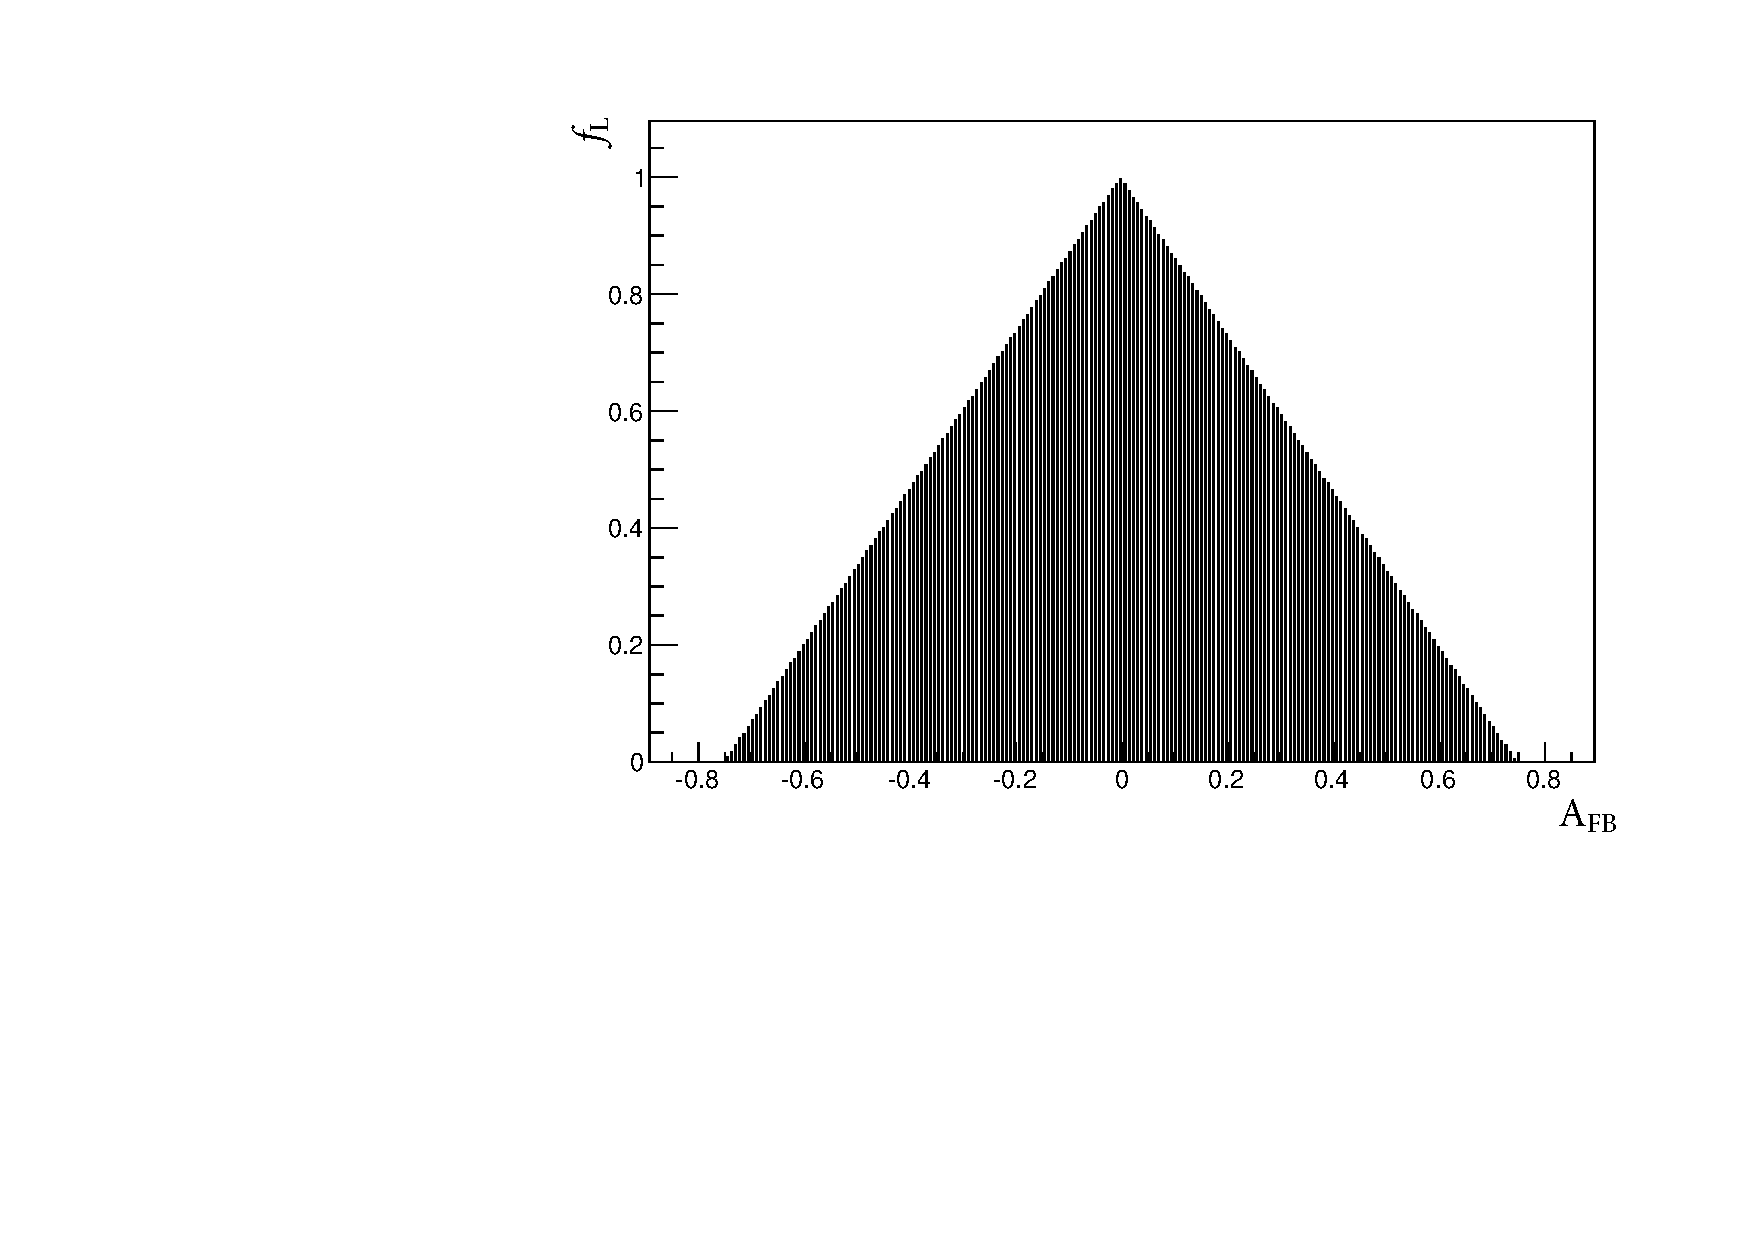
\includegraphics[width=0.8\textwidth]{Lmumu/figs/scan.pdf}
\caption{The physical ($A_{\rm FB}^\ell$,$f_{\rm L}$) parameter space. The dark region corresponds 
to points where the PDF is positive in the whole $[-1,1]$ interval. }
\label{fig:pdfscan}
\end{figure}


\section{Feldman-cousins plug-in method}
\label{sec:FeldmanCousins}

Physical boundaries of the parameter space could result in a wrong estimation of the uncertainties,
especially if the measured value is close to the border. To deal with this effects the 
likelihood-ordering method~\cite{Feldman:1997qc} is used to estimate uncertainties in this analysis and
nuisance parameters are accounted for using the plug-in method~\cite{Karbach:2011uz}. This is a unified 
method to calculate confidence intervals and upper/lower limits, based on simulated experiments and has 
the advantage of having a well defined frequentist coverage.

%One defines two classes of parameters: Parameters of Interest (PoI), which are those for which
%one wants to construct confidence intervals, and nuisance parameters, which are all the secondary
%parameters in a model. In our analysis the baryon side has one parameter only, $A_{\rm FB}^h$, 
%which we consider PoI and the lepton side has two which we alternatively consider PoI and nuisance. 

The method is constituted by the following steps:
\begin{enumerate}
\item fit real data distributions with all parameters free;
\item fit real data fixing the PoIs to a value of choice and keeping nuisance parameters free;
\item generate simulated samples following the distribution given by the fit model,
where all nuisance parameters are taken from the fit in point 2 and PoIs are fixed to the same value used in point 2;
\item repeat the two fits made on data on each simulated sample: fit with all parameters free and with fixed PoIs;
\item extract the value of the Log-Likelihoods at the minimum for all cases;
\item calculate the percentage of simulated experiments in which the ratio
$\log\mathcal{L}_{fixed}/\log\mathcal{L}_{free}$ is bigger than in data.
\item repeat the procedure for many values of the PoIs scanning around the best fit values.
\end{enumerate}

The confidence interval at $k\%$ is given by the points where the free-to-fixed likelihood ratio is bigger in data than
simulation for $(1-k)\%$ of times. As an example, in Fig.~\ref{fig:FCexample} are reported the p-values obtained
with the plug-in method for $A_{\rm FB}^\ell$ and $f_{\rm L}$. For the analysis the two-dimensional allowed region 
is scanned giving a grid of p-values, which translated into two-dimensional confidence regions.
%
\begin{figure}[h!]
\centering
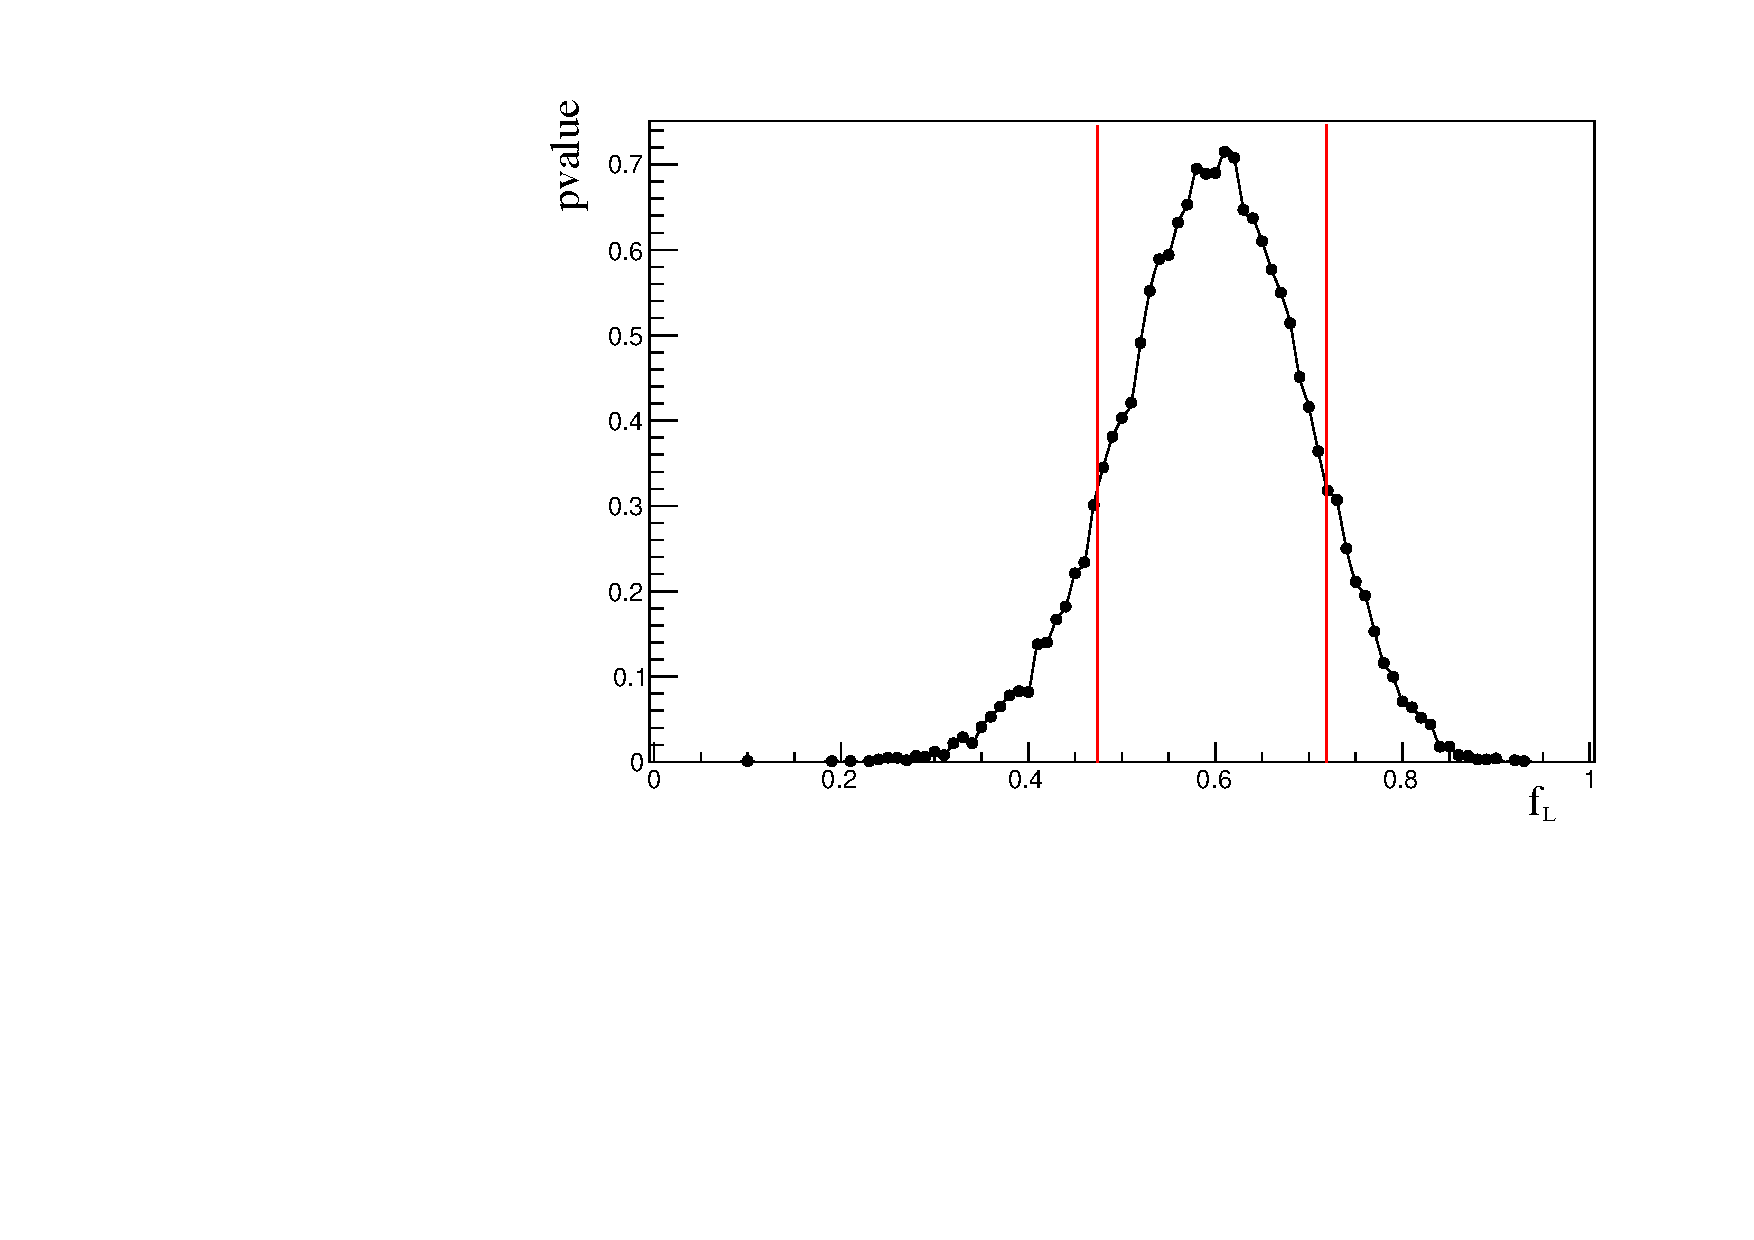
\includegraphics[width=0.48\textwidth]{Lmumu/figs/pvalue_fL_1500_2000.pdf}
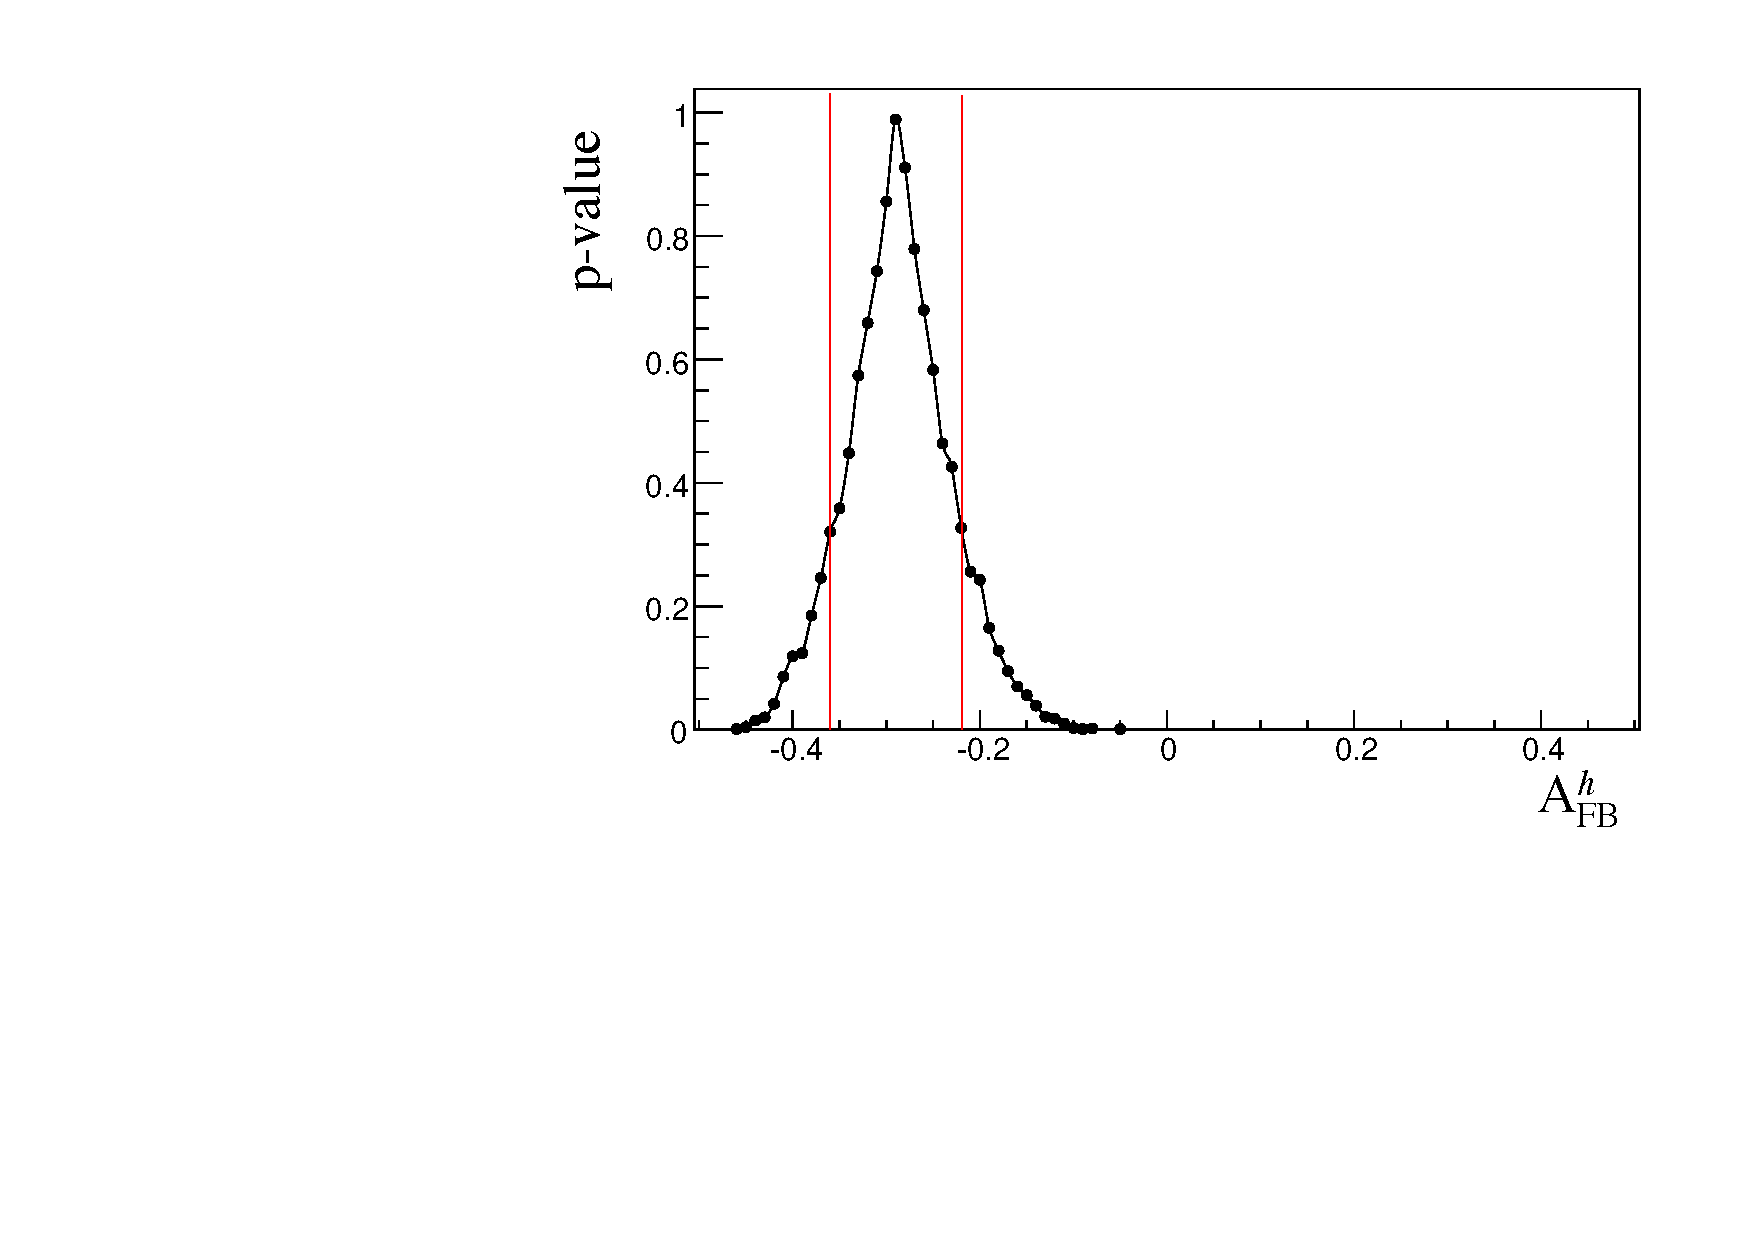
\includegraphics[width=0.48\textwidth]{Lmumu/figs/pvalue_afbB_1500_2000.pdf}
\caption{ Dependence of the p-value from the values of the angular observables $f_{\rm L}$ (left) 
and $A_{\rm FB}^h$ (right) in simulated experiments. The red lines mark the points
at p-value 32\% corresponding to a 68\% CL.}
\label{fig:FCexample}
\end{figure}

\section{Modelling the angular distributions}
\label{sec:angfit}

The observables are extracted from fits to one-dimensional angular distributions.
%
%The function describing the $\cos\theta_\ell$ distribution, used to extract $A_{\rm FB}^\ell$ is 
%given by (for details, see appendix \ref{ap:angObservables})
%\begin{align}
%\frac{d\Gamma(\Lambda_{b}\to \Lambda \,\ell^{+}\ell^{-})}{dq^2d\cos\theta_\ell}=
%\frac{d\Gamma}{dq^2}&\left[  \frac{3}{8}\left(1+\cos^2\theta_\ell\right)(1-f_{\rm L})+A_{\rm FB}^\ell\cos\theta_\ell +
%   \frac{3}{4}f_{\rm L} \sin^2\theta_\ell \right], 
%\label{eq:afbLTh}
%\end{align}
%where $f_{\rm L}$ is fraction of longitudinally polarised dimuons.
%The distribution for the hadronic side has form
%\begin{equation}
%\frac{d\Gamma(\Lambda_{b}\to \Lambda(\to p \pi^{-})\ell^{+}\ell^{-})}
%     {dq^2\,d\cos\theta_\Lambda} 
%={\rm Br}(\Lambda \to p\pi^{-})
% \frac{d\Gamma(\Lambda_b \to \Lambda\, \ell^{+}\ell^{-})}{d q^2}\frac{1}{2}
%\Big(1+2A_{\rm FB}^h\cos\theta_\Lambda\Big) \,. 
%\label{eq:afbBTh}
%\end{equation}
%
The PDFs used to model the data are defined as
%
\begin{equation}
P^k(\cos\theta_{\ell/h}) = f_b P_S(\cos\theta_{\ell/h}) \times \varepsilon^k(\cos \theta_{\ell/h}) + 
		(1-f_b)P_B^k(\cos\theta_{\ell/h}),
\end{equation}
%
where $k=$(LL,DD), $P_S$ is the signal function composed by a theoretical shape given by Eq.~\ref{eq:afbBTh}
and~\ref{eq:afbLTh}, which is multiplied by an acceptance function $\varepsilon$ described in Sec.~\ref{sec:AngEff}
and $P_B$ is a background component. To limit systematic effects due to the background parameterisation, 
the fit is performed in a restricted mass region around the peak:
$5580 < m(\Lz\mumu) < 5660 $ \mevcc ~(``signal region"), which is dominated by the signal.
%In this way in most of the \qsq bins we have $\sim 20\%$ of background events.
The background fraction, $f_b$, is obtained by looking at the 4-body $m(p\pi\mu\mu)$ invariant mass
distribution in a wider interval and fitting it to extract the fraction of background in the signal region.
In the fit to the angular distributions this is then gaussian constrained to the obtained value.
The background shape is parameterised with a linear function times the efficiency shape.
A different efficiency shape is used for downstream and long events and for each \qsq interval.
The free parameter of this model is fitted on sideband candidates which contain only background
and fixed for the fit to the signal region. Figure~\ref{fig:cosThetaLbkg}
reports the background distributions in the sideband, $m(p\pi\mumu) > 5700$ \mevcc,
for the high \qsq integrated interval with overlaid the background function.
In summary the only fit parameter in the total fit function is the forward-backward asymmetry
(and $f_{\rm L}$ in the leptonic case). 

\begin{figure}[h]
\centering
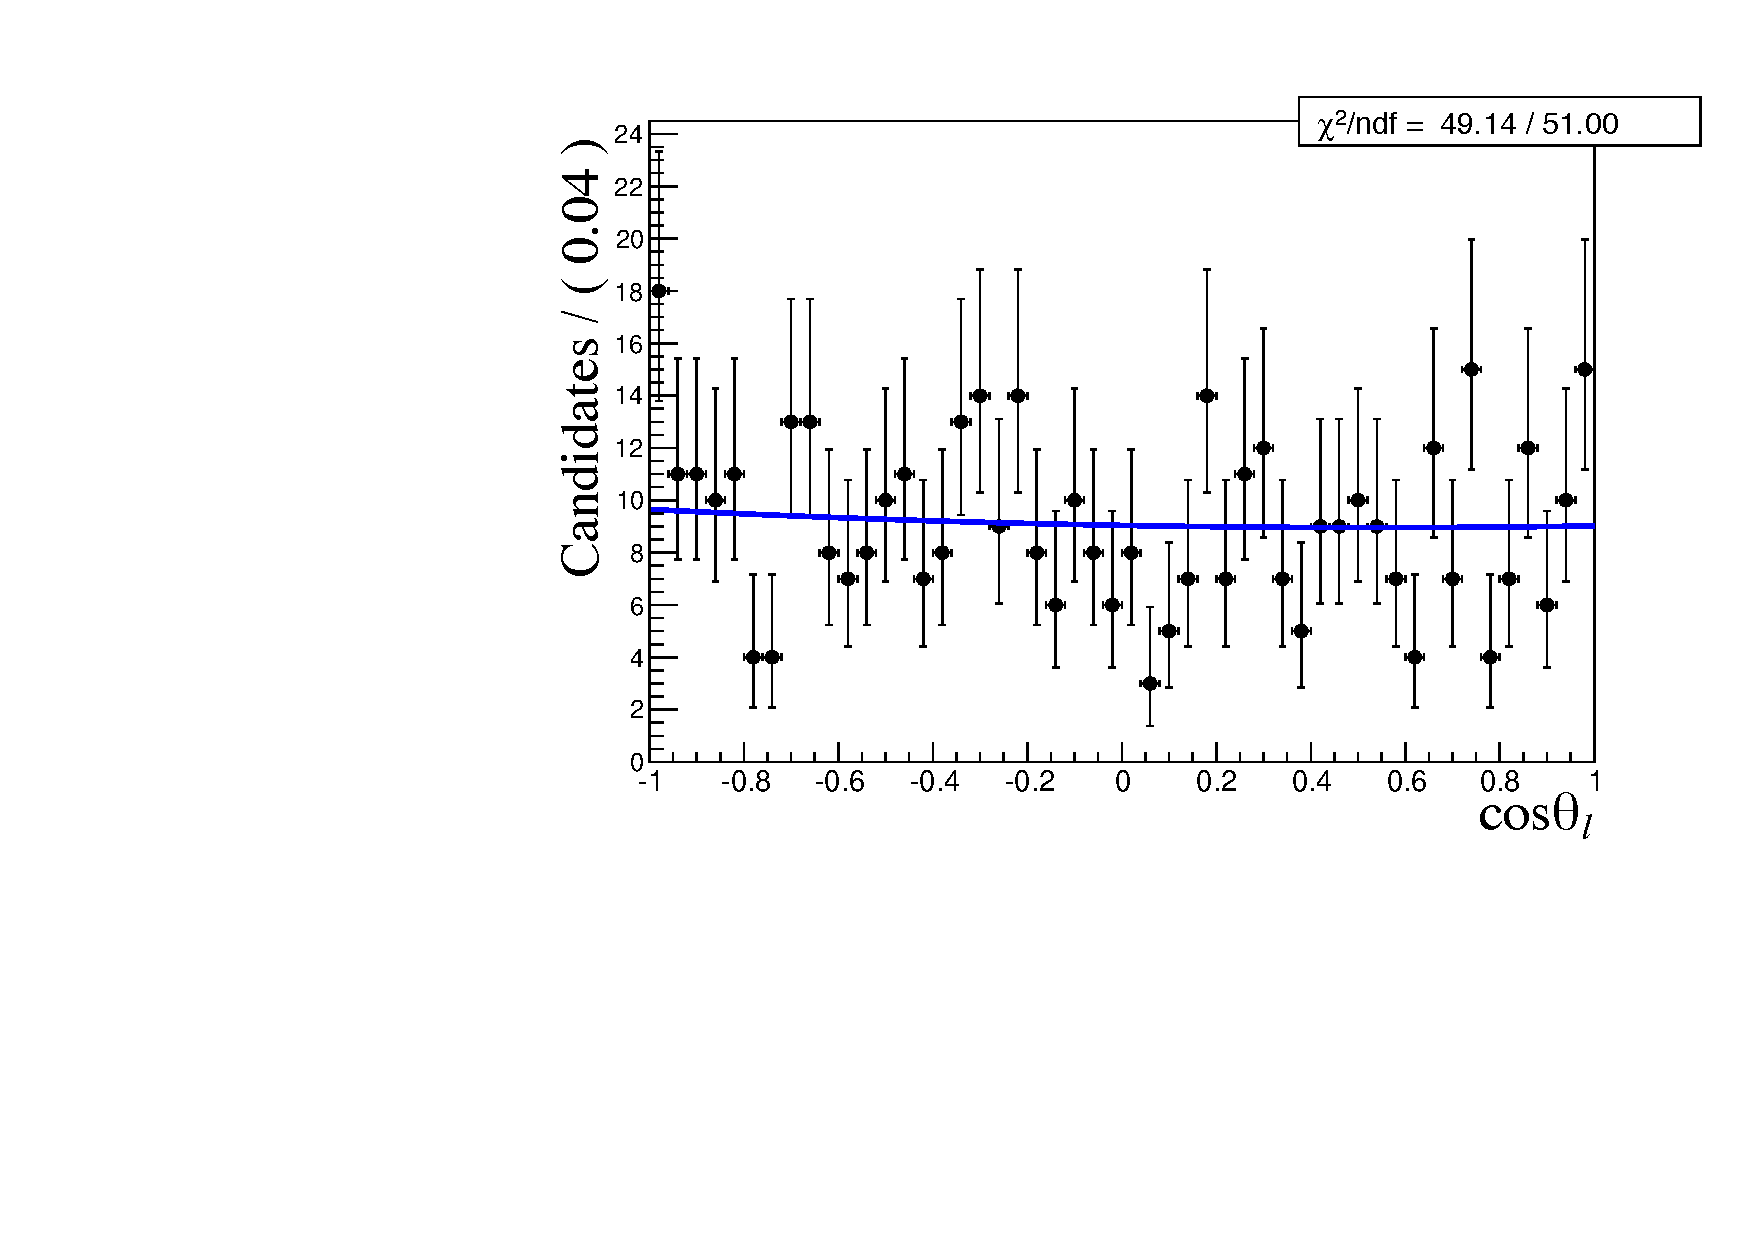
\includegraphics[width=0.48\textwidth]{Lmumu/figs/AngularBkgFits/BkgFit_highq2_DD.pdf}
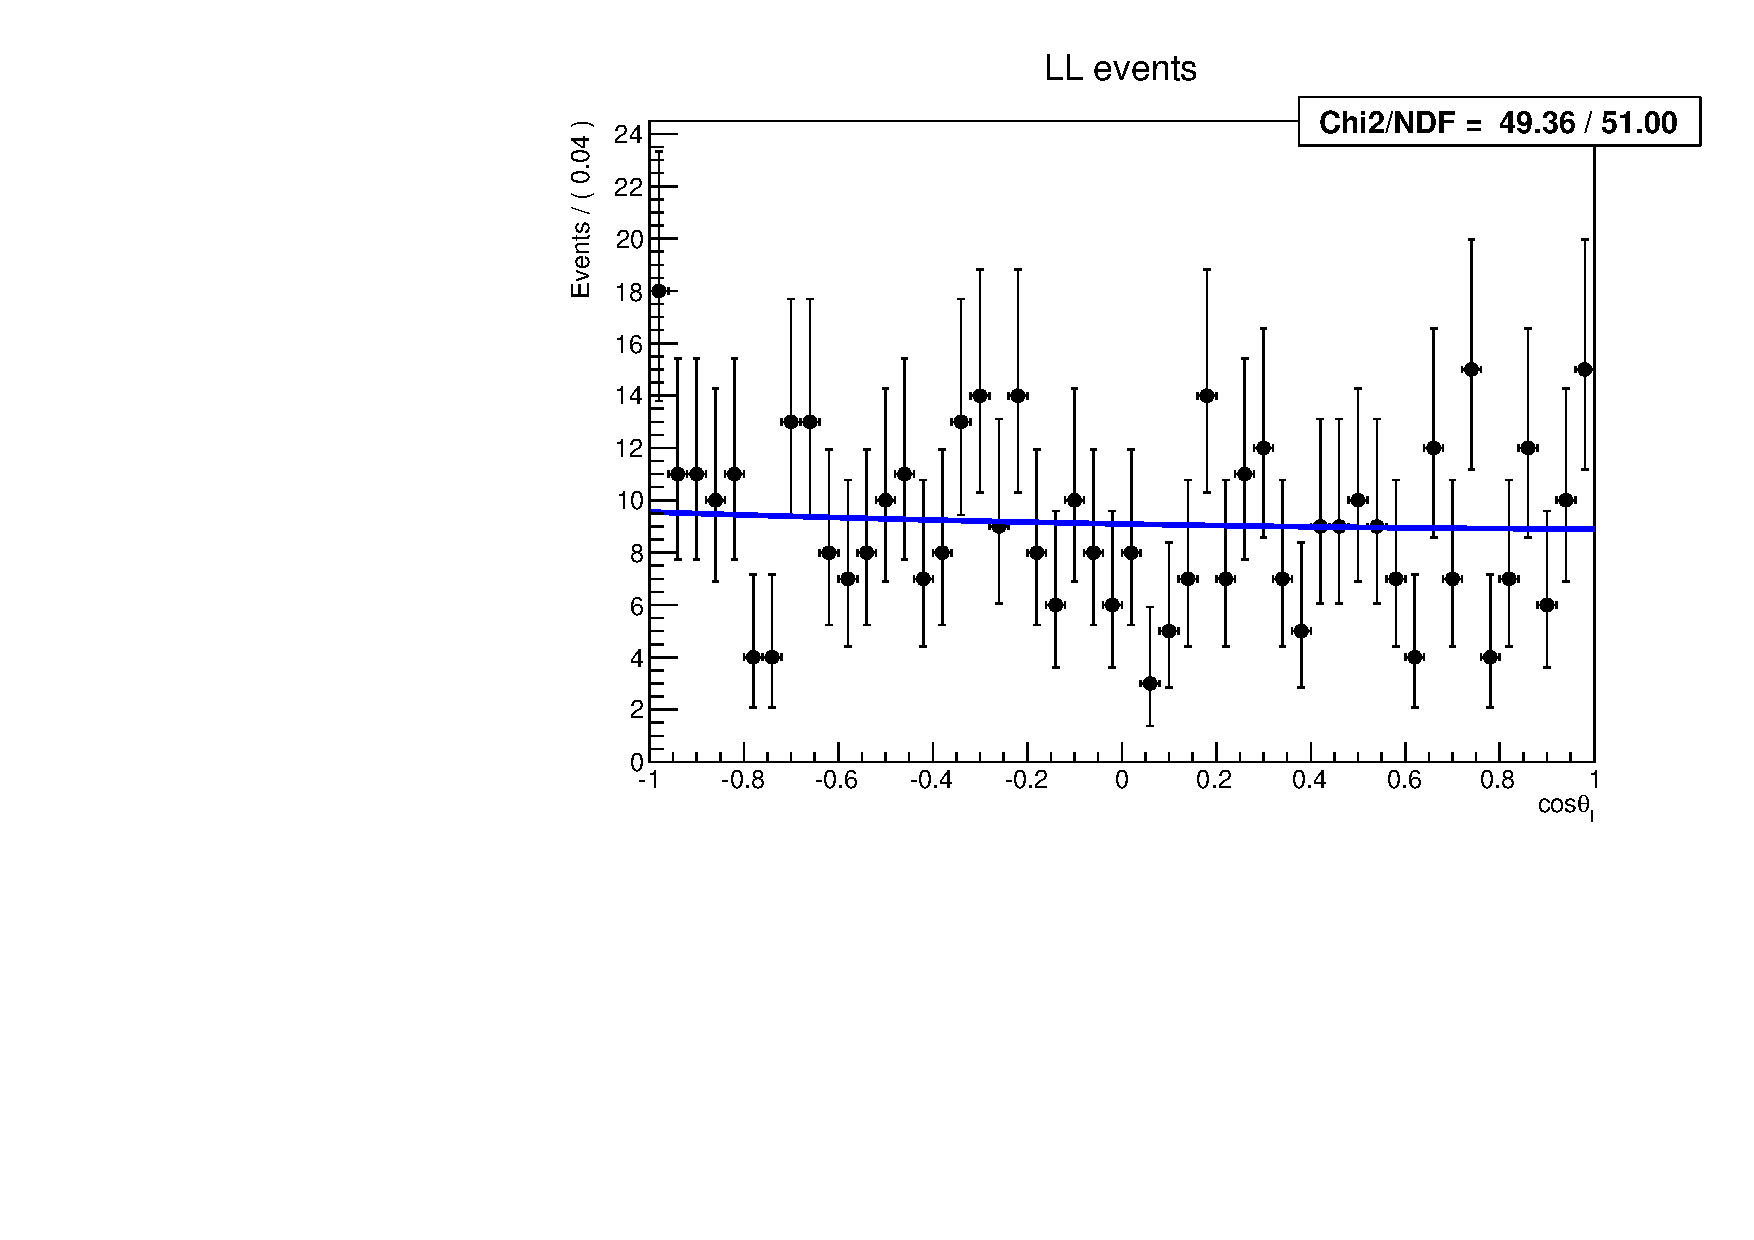
\includegraphics[width=0.48\textwidth]{Lmumu/figs/AngularBkgFits/BkgFit_highq2_LL.pdf}
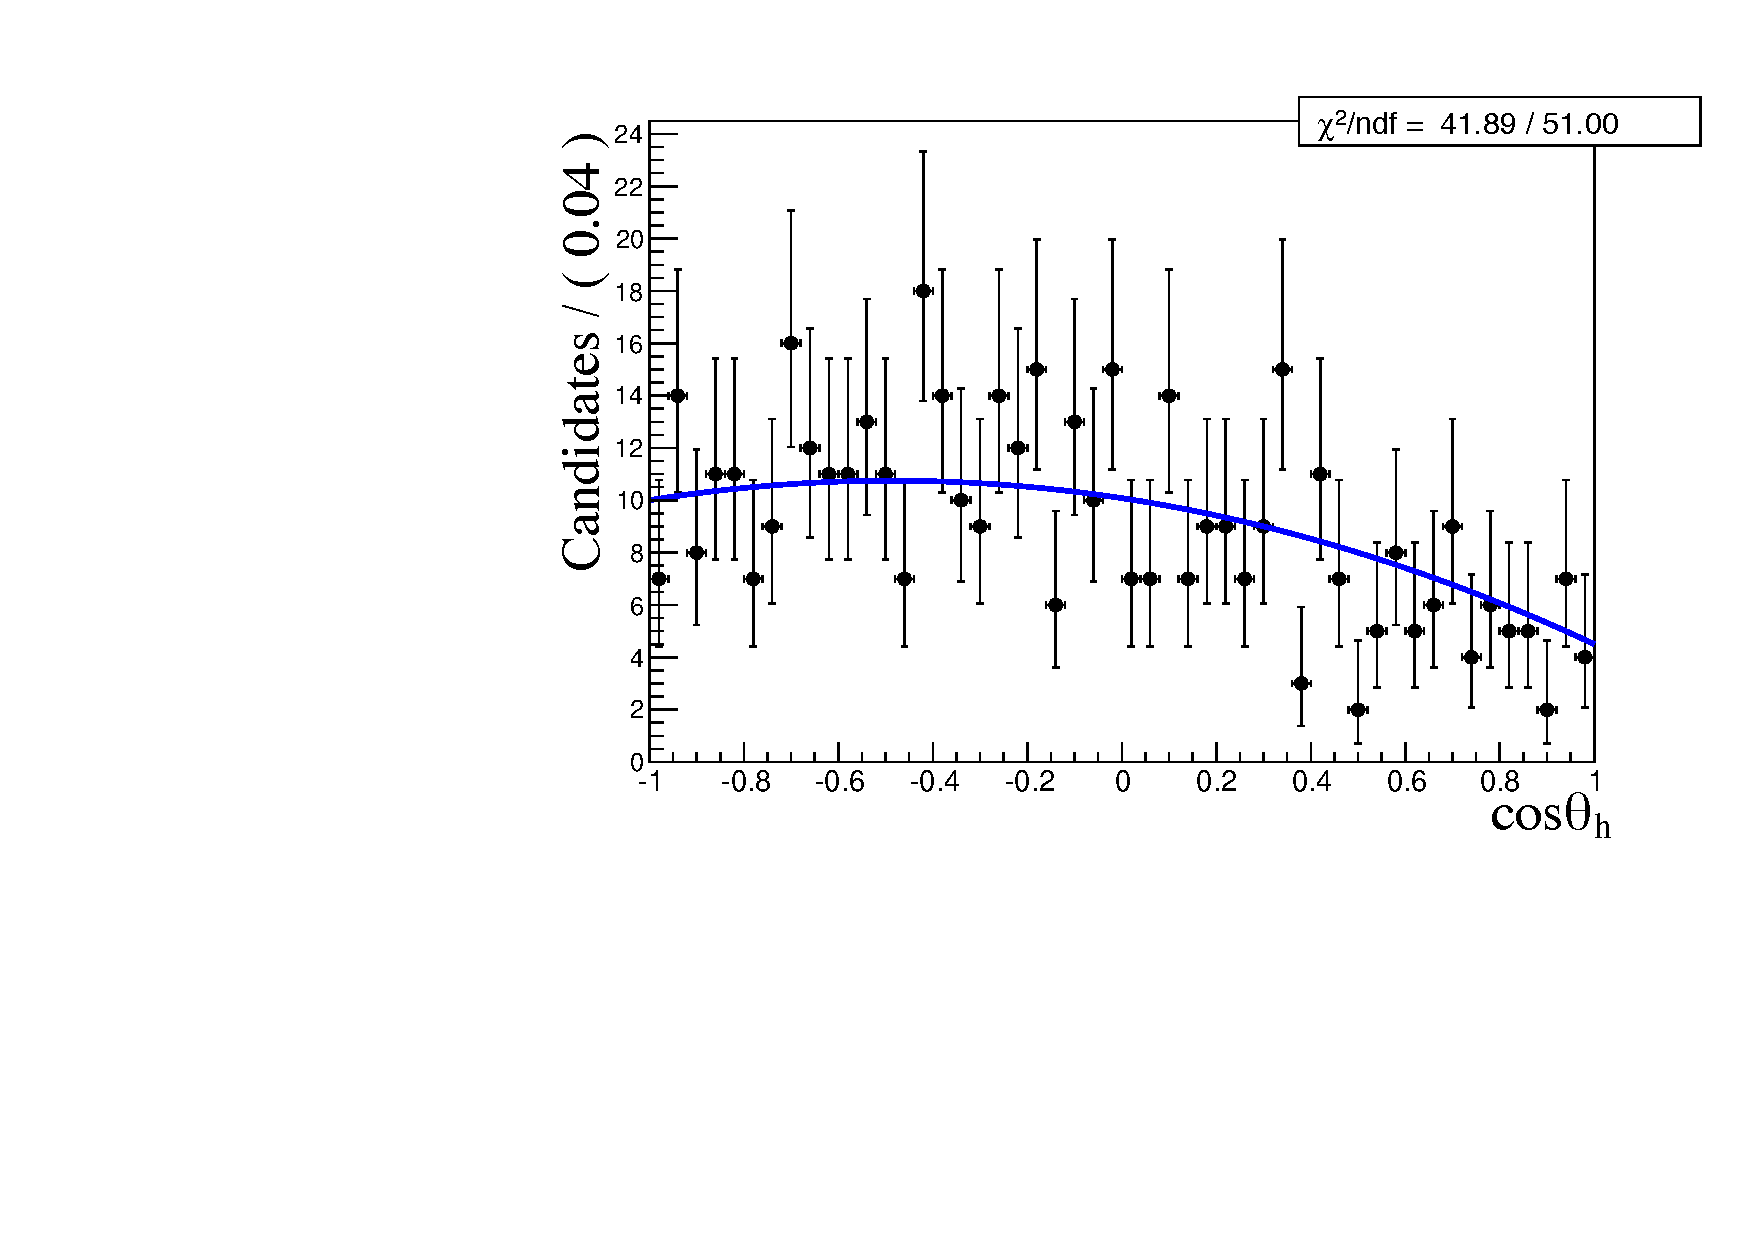
\includegraphics[width=0.48\textwidth]{Lmumu/figs/AngularBkgFits/BkgFitB_highq2_DD.pdf}
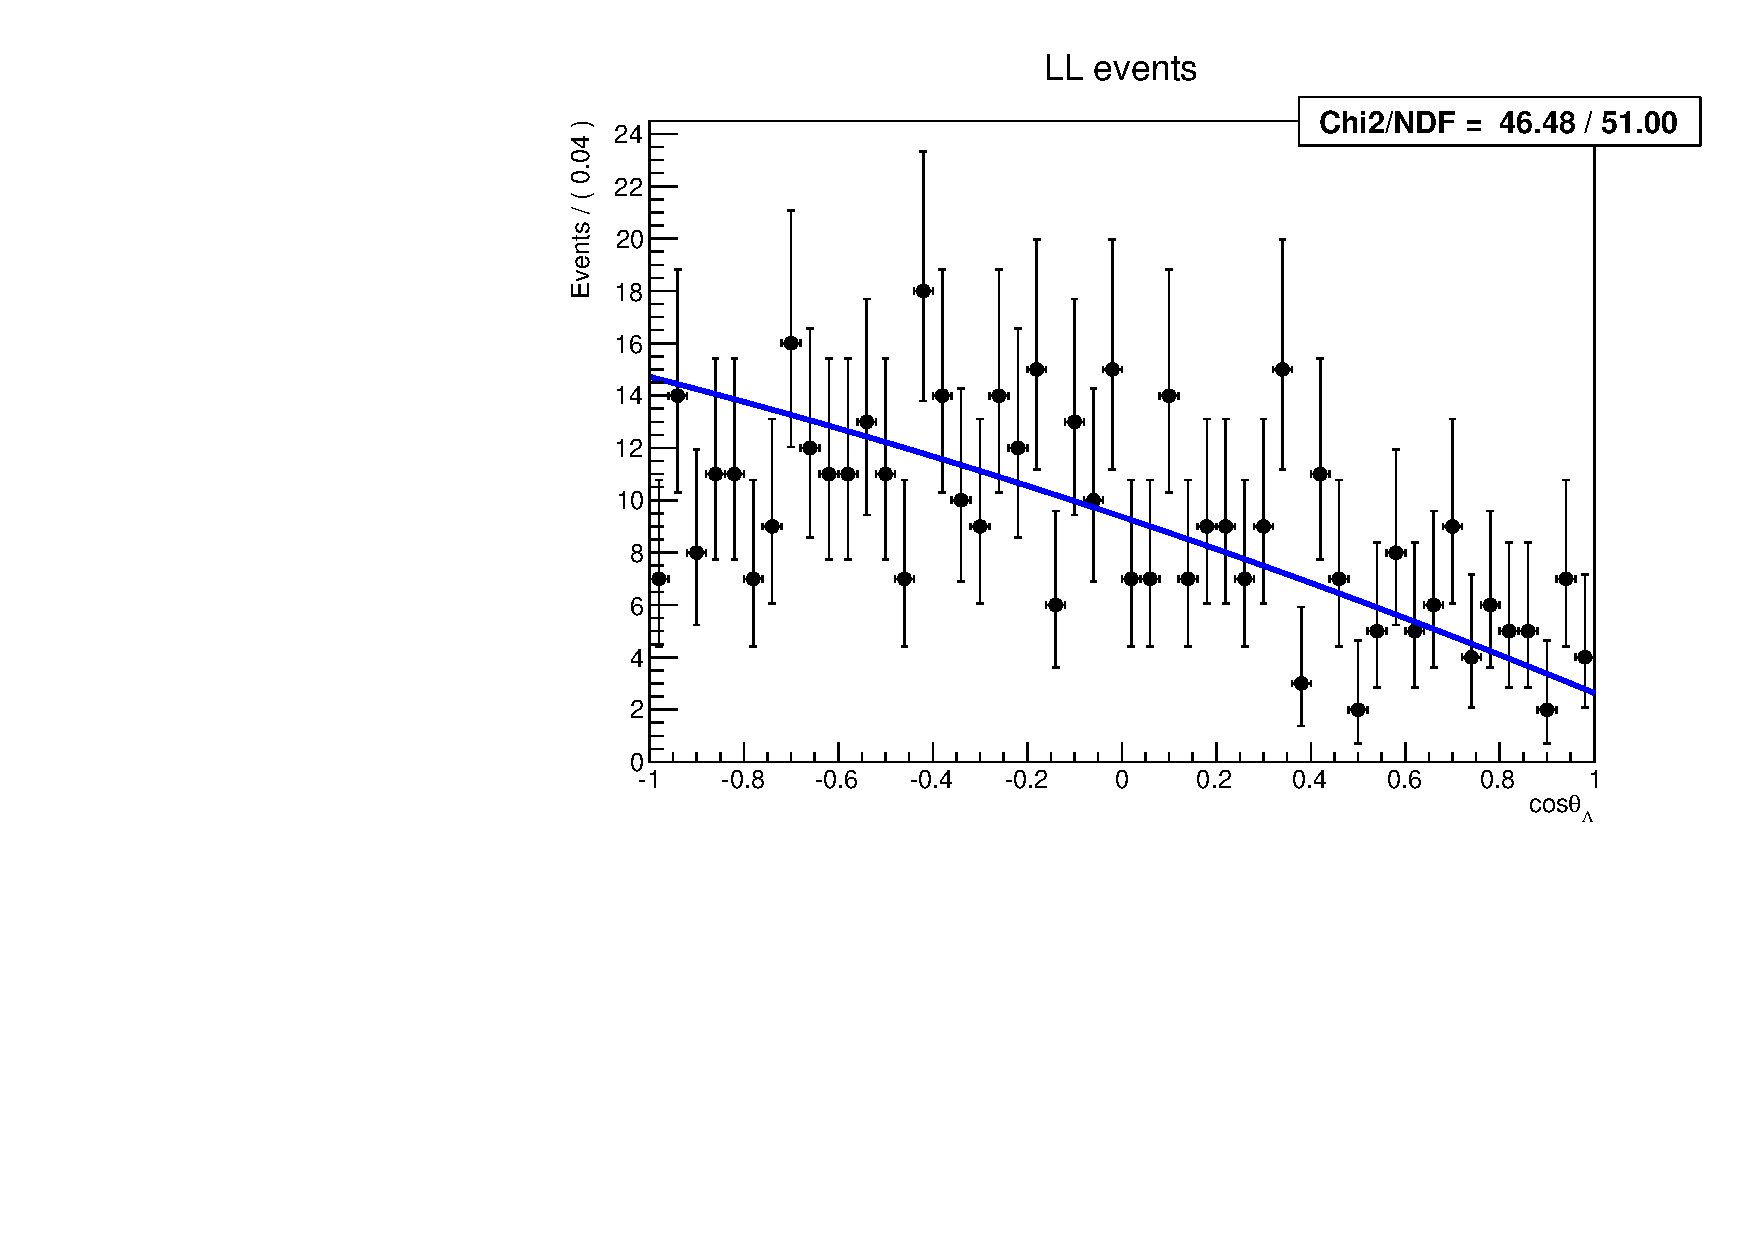
\includegraphics[width=0.48\textwidth]{Lmumu/figs/AngularBkgFits/BkgFitB_highq2_LL.pdf}
\caption{Background distribution as a function of $\cos\theta_\ell$ (top) and $\cos\theta_h$ (bottom)
for downstream (left) and long (right) candidates in the 15-20 \gevgevcccc ~\qsq interval.  }
\label{fig:cosThetaLbkg}
\end{figure}

%\begin{figure}[h]
%\centering
%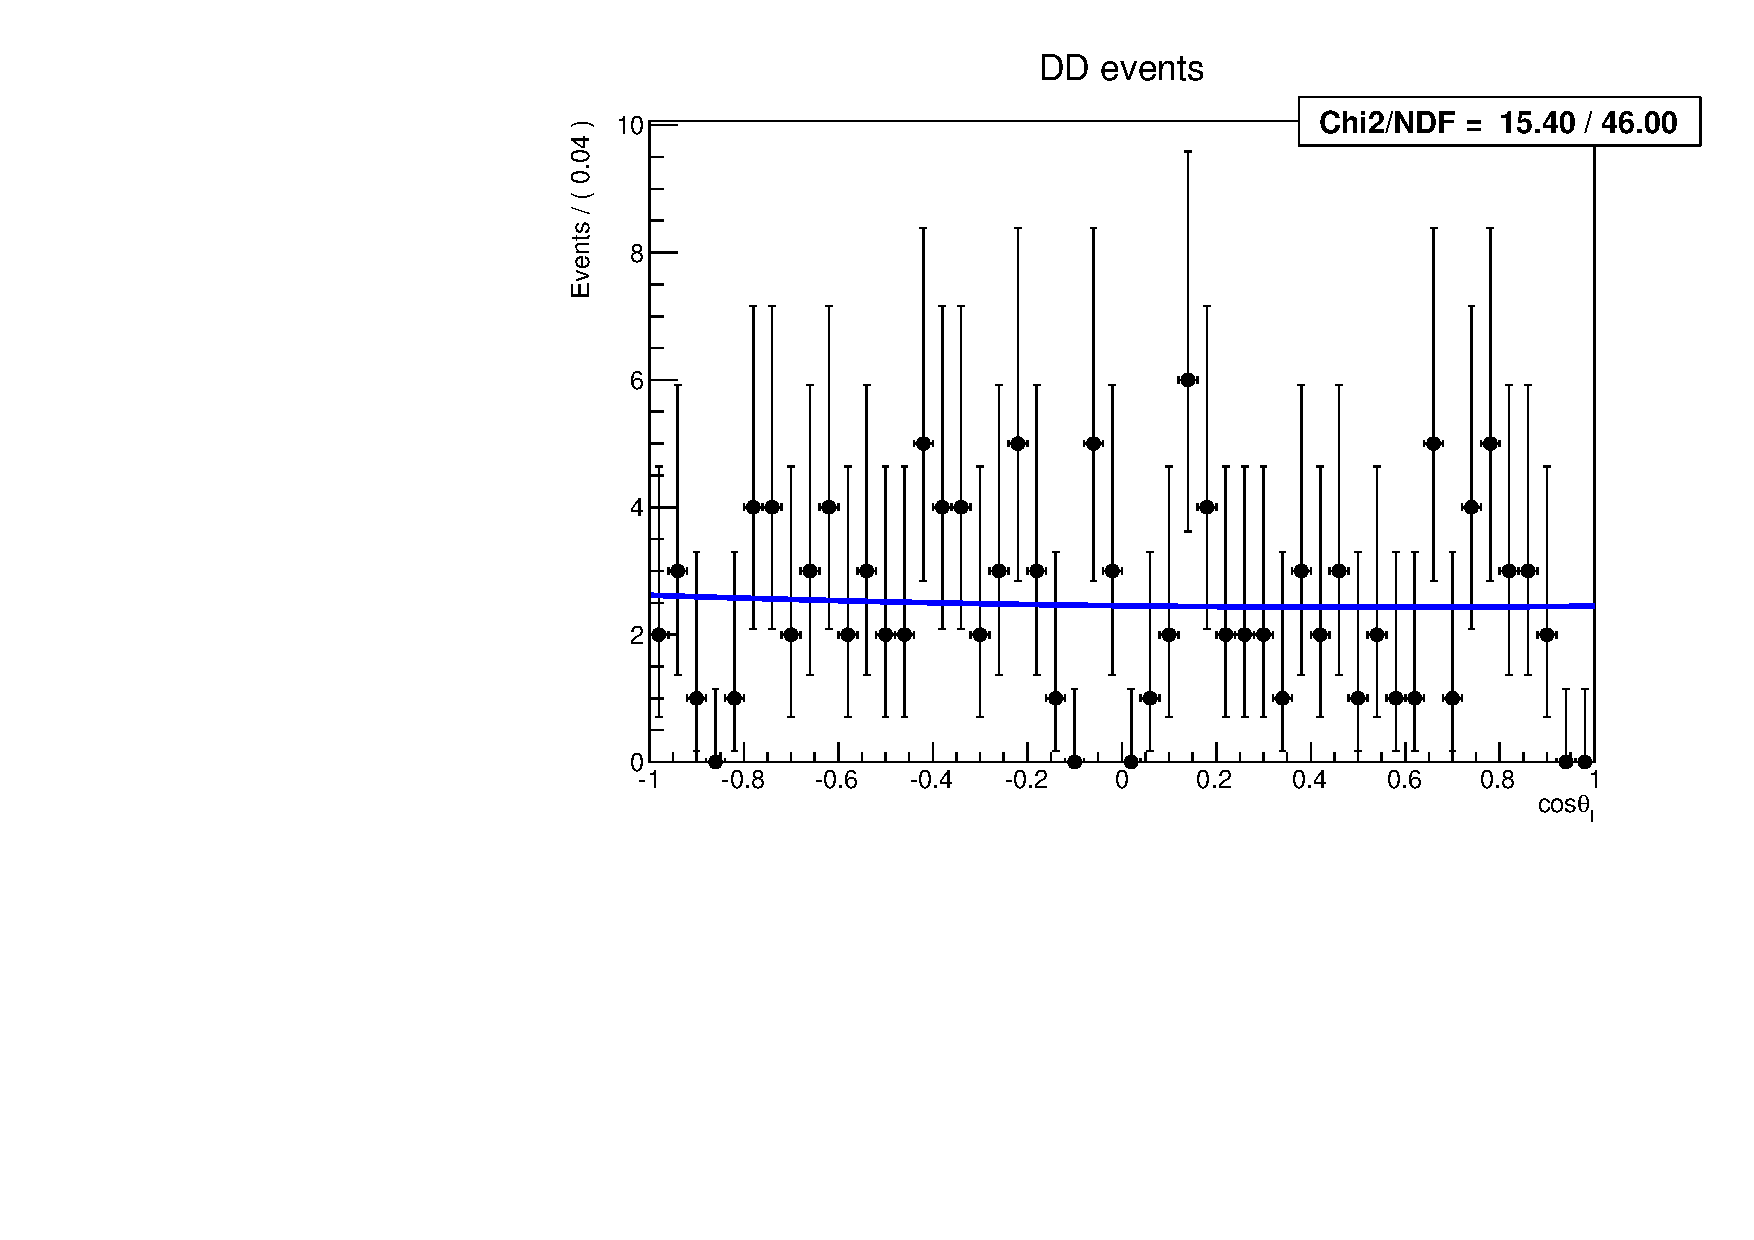
\includegraphics[width=0.45\textwidth]{Lmumu/figs/AngularBkgFits/BkgFit_lowq2_DD.pdf}
%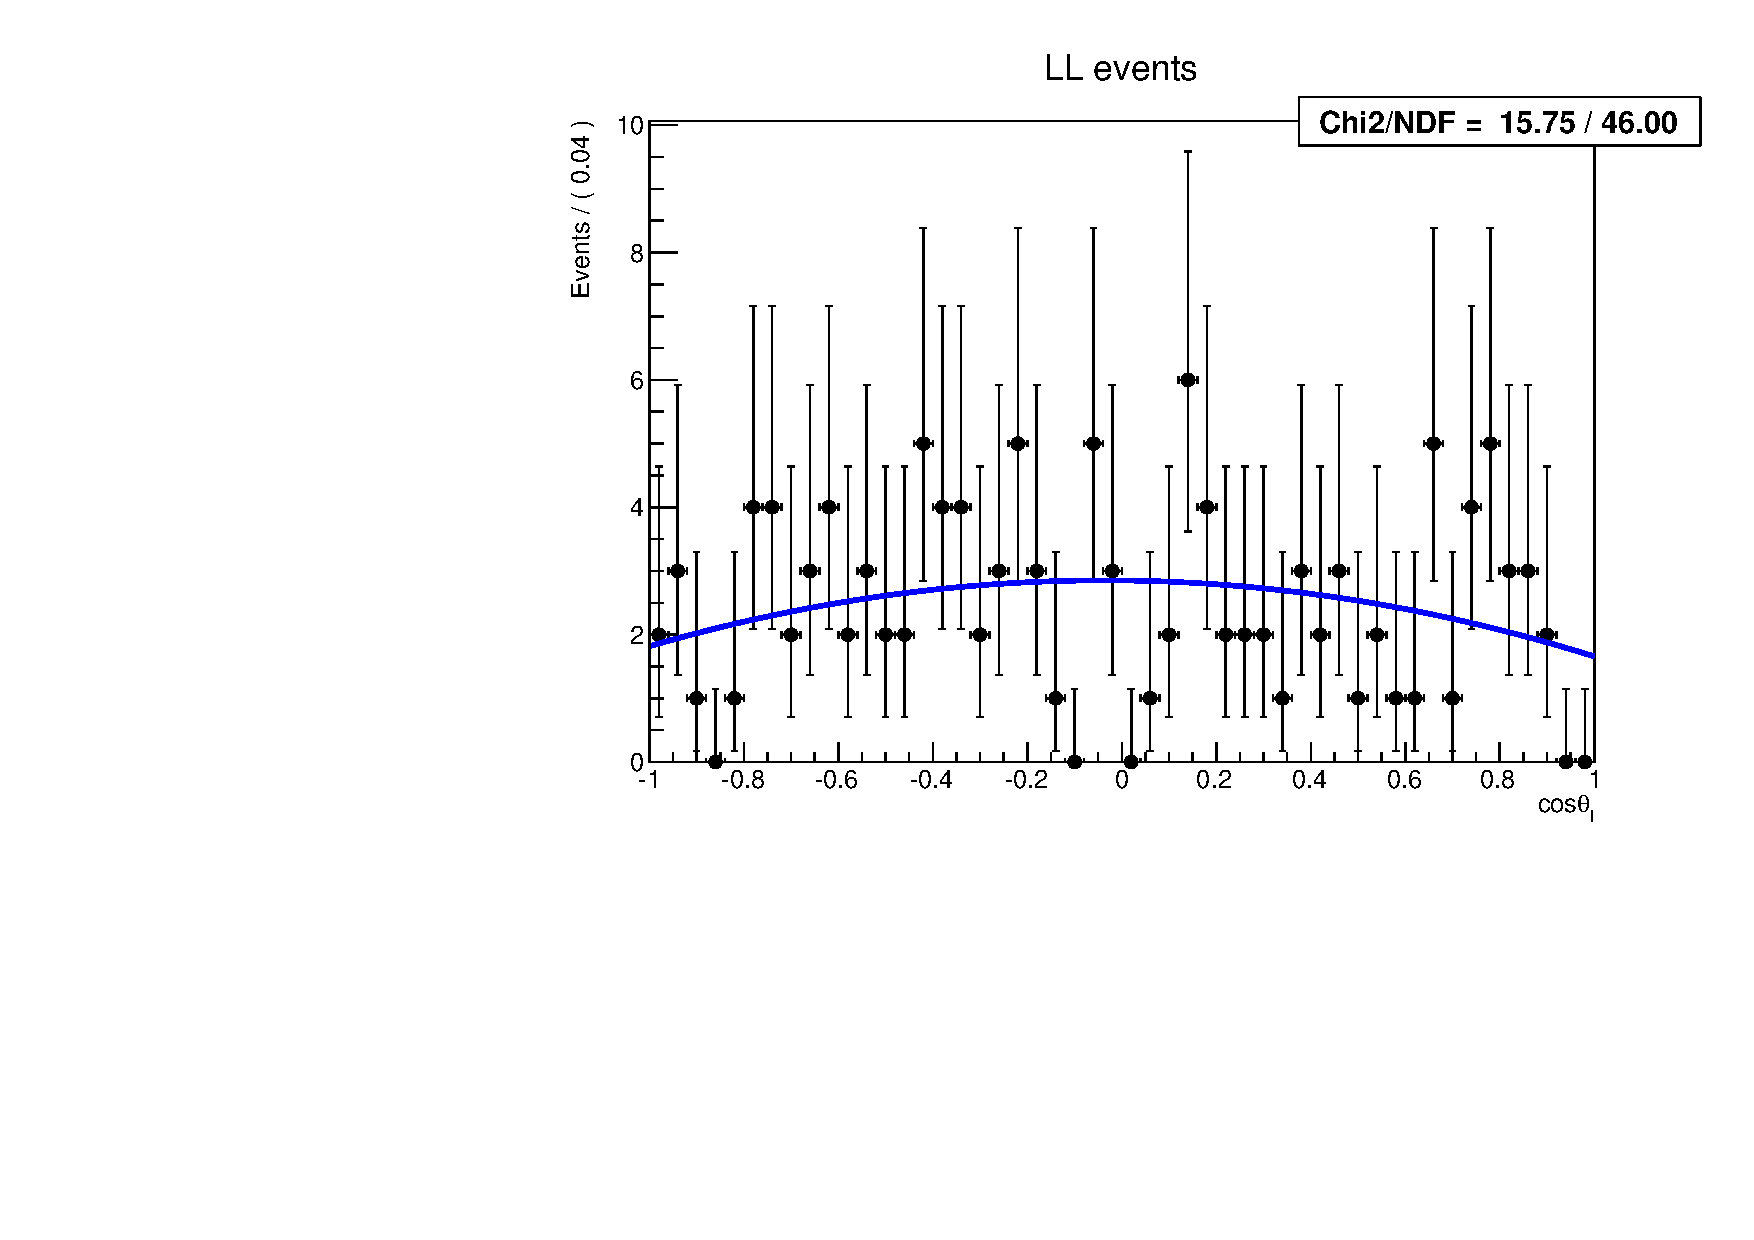
\includegraphics[width=0.45\textwidth]{Lmumu/figs/AngularBkgFits/BkgFit_lowq2_LL.pdf}
%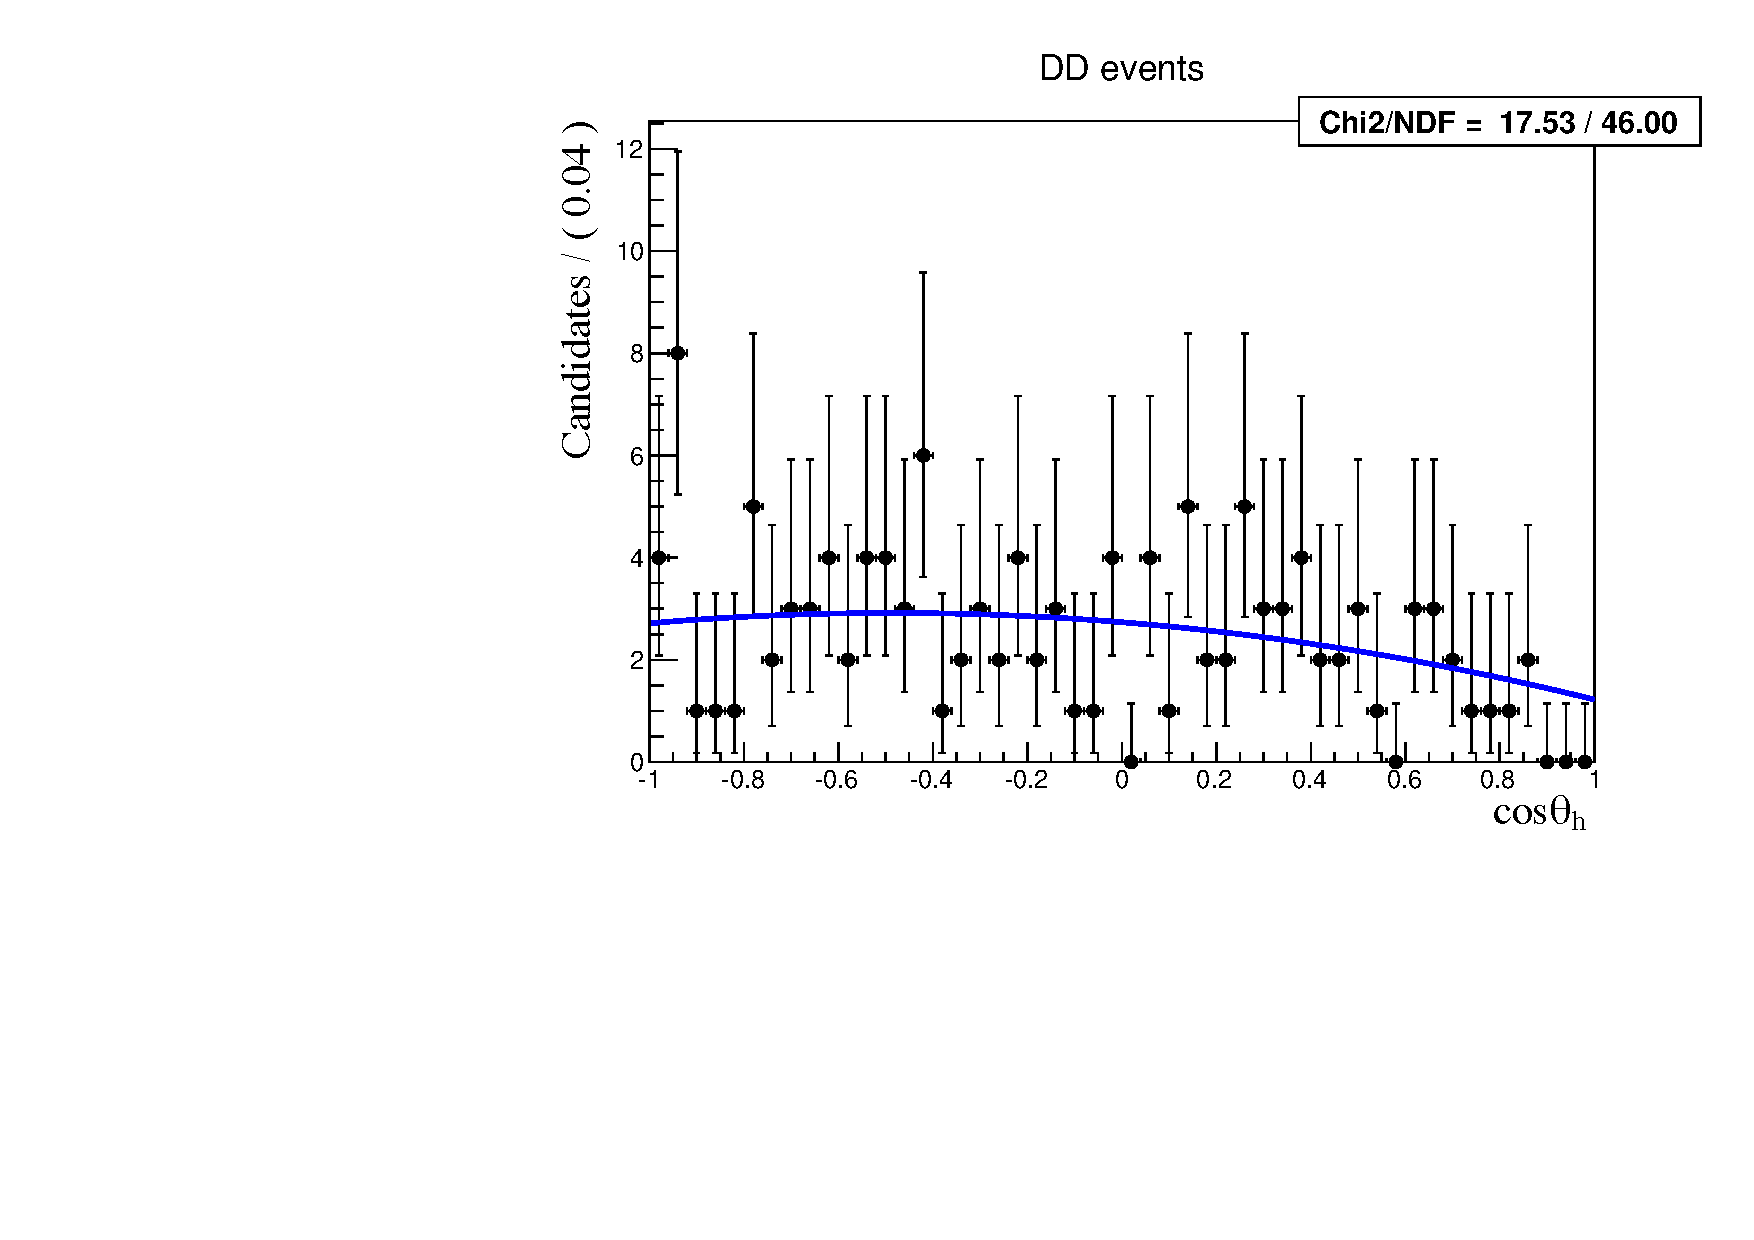
\includegraphics[width=0.45\textwidth]{Lmumu/figs/AngularBkgFits/BkgFitB_lowq2_DD.pdf}
%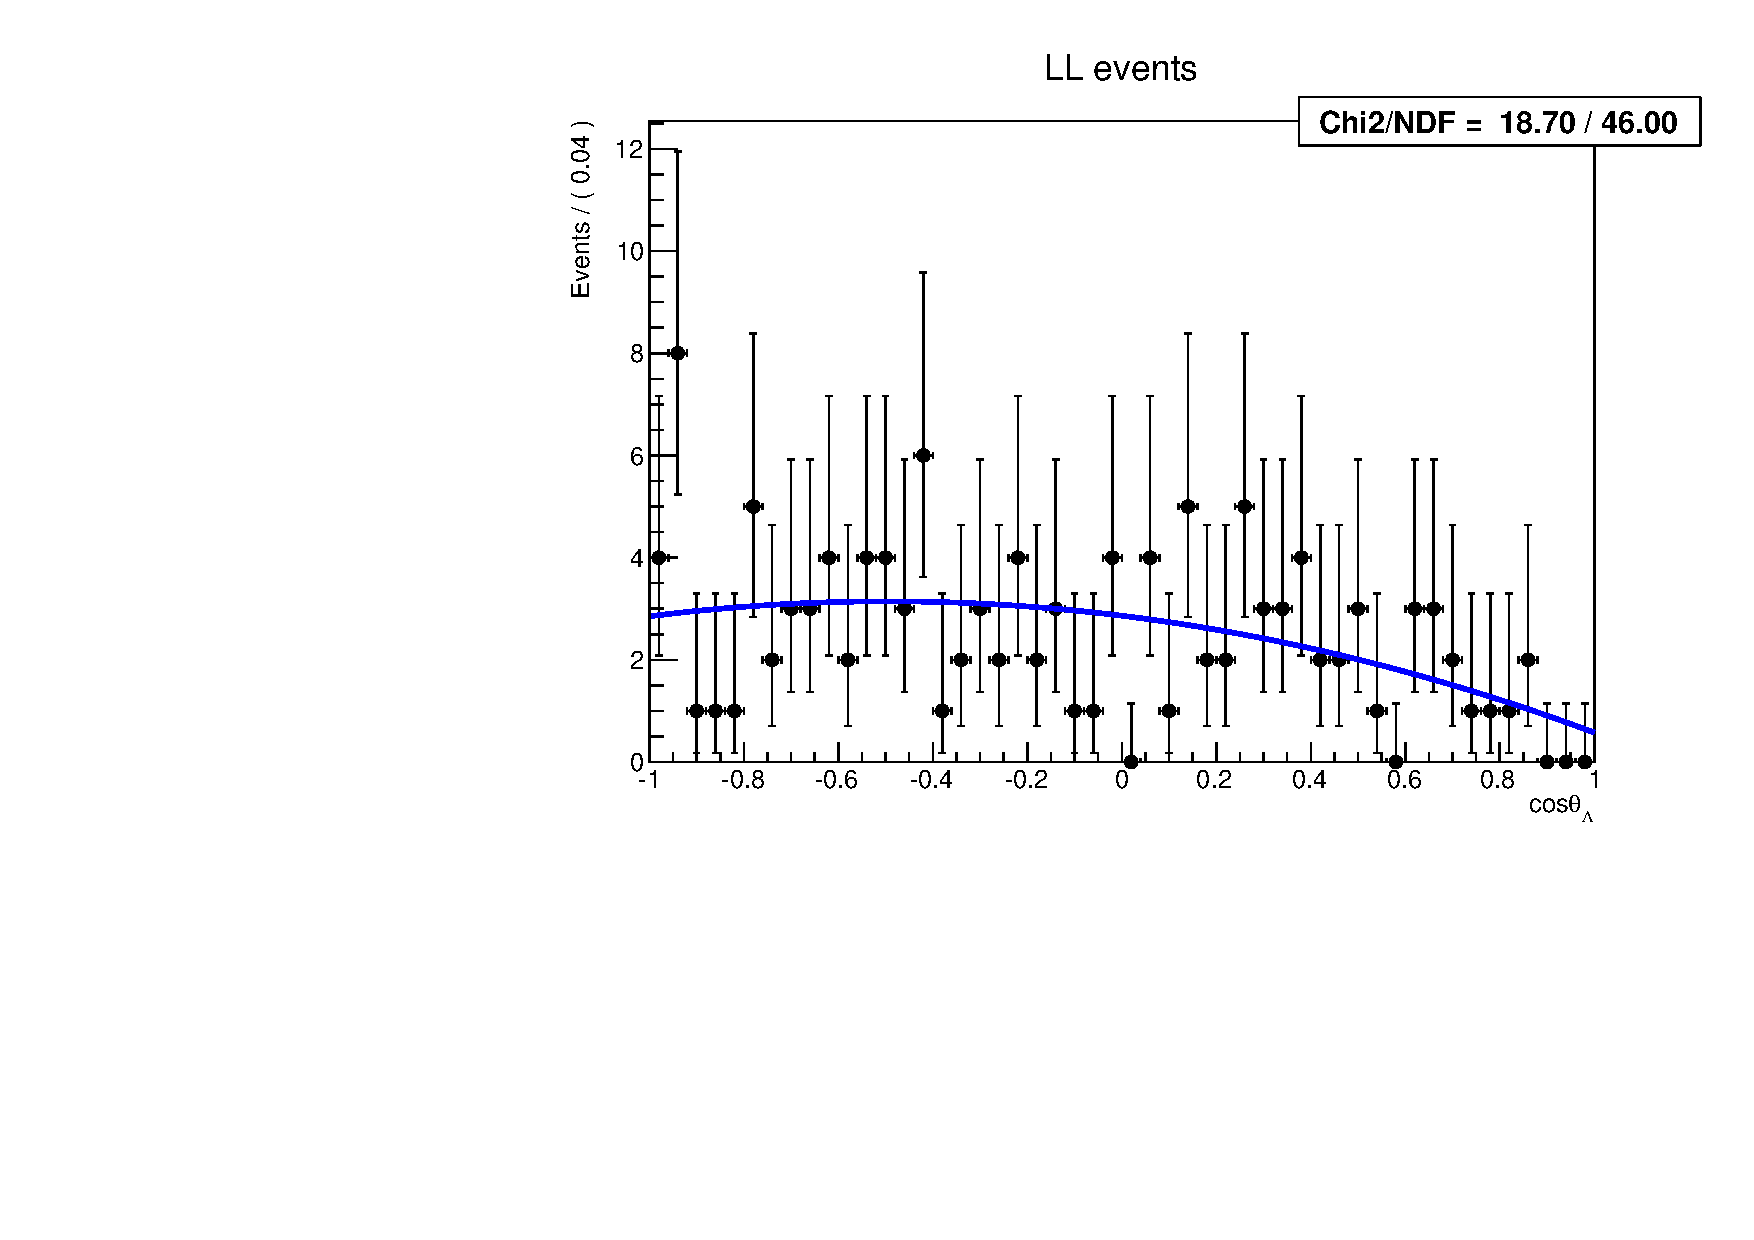
\includegraphics[width=0.45\textwidth]{Lmumu/figs/AngularBkgFits/BkgFitB_lowq2_LL.pdf}
%\caption{Background distribution as a function of $\cos\theta_\Lambda$ for downstream (left) and long (right)
%events in the 15-20 \gevgevcccc (top) and 1.1-6 \gevgevcccc (bottom) \qsq bins. }
%\label{fig:cosThetaBbkg}
%\end{figure}


\section{Angular acceptance}
\label{sec:AngEff}

Selection requirements on the minimum momentum of the muons may distort the $\cos\theta_\ell$ 
distribution by removing candidates with extreme values of $\cos\theta_\ell$. Similarly, 
the impact parameter requirements affect $\cos\theta_h$ as very forward hadrons tend
to have smaller impact parameter values. While in principle one could take it into account
by an additional weight, to minimise the distortion of the uncertainties estimate,
the efficiency function is incorporated in the fit model. The angular efficiency is
parametrised using a second-order polynomial and determined separately for downstream and
long candidates by fitting simulated events, with an independent set of parameters obtained
for each \qsq interval. These parameters are fixed for the fits to data.
Using polynomial functions allows to calculate the PDF normalisation analytically.
Figure~\ref{fig:angular_eff} shows total efficiency as a function of $\cos\theta_h$ and 
$\cos\theta_\ell$ in the 15.0--20.0 integrated \qsq interval obtained using a $\Lb\to\Lz\mumu$ simulated sample.
%$\ref{fig:cosThetaLeffJpsi} and \ref{fig:cosThetaBeffJpsi} $J/\psi\Lz$ MC and $\Lz\mumu$ 
%
For the lepton side, even though the efficiency is symmetric by construction,
all parameters are left free to float, namely it is not constrained to be symmetric.

\begin{figure}[h]
\centering
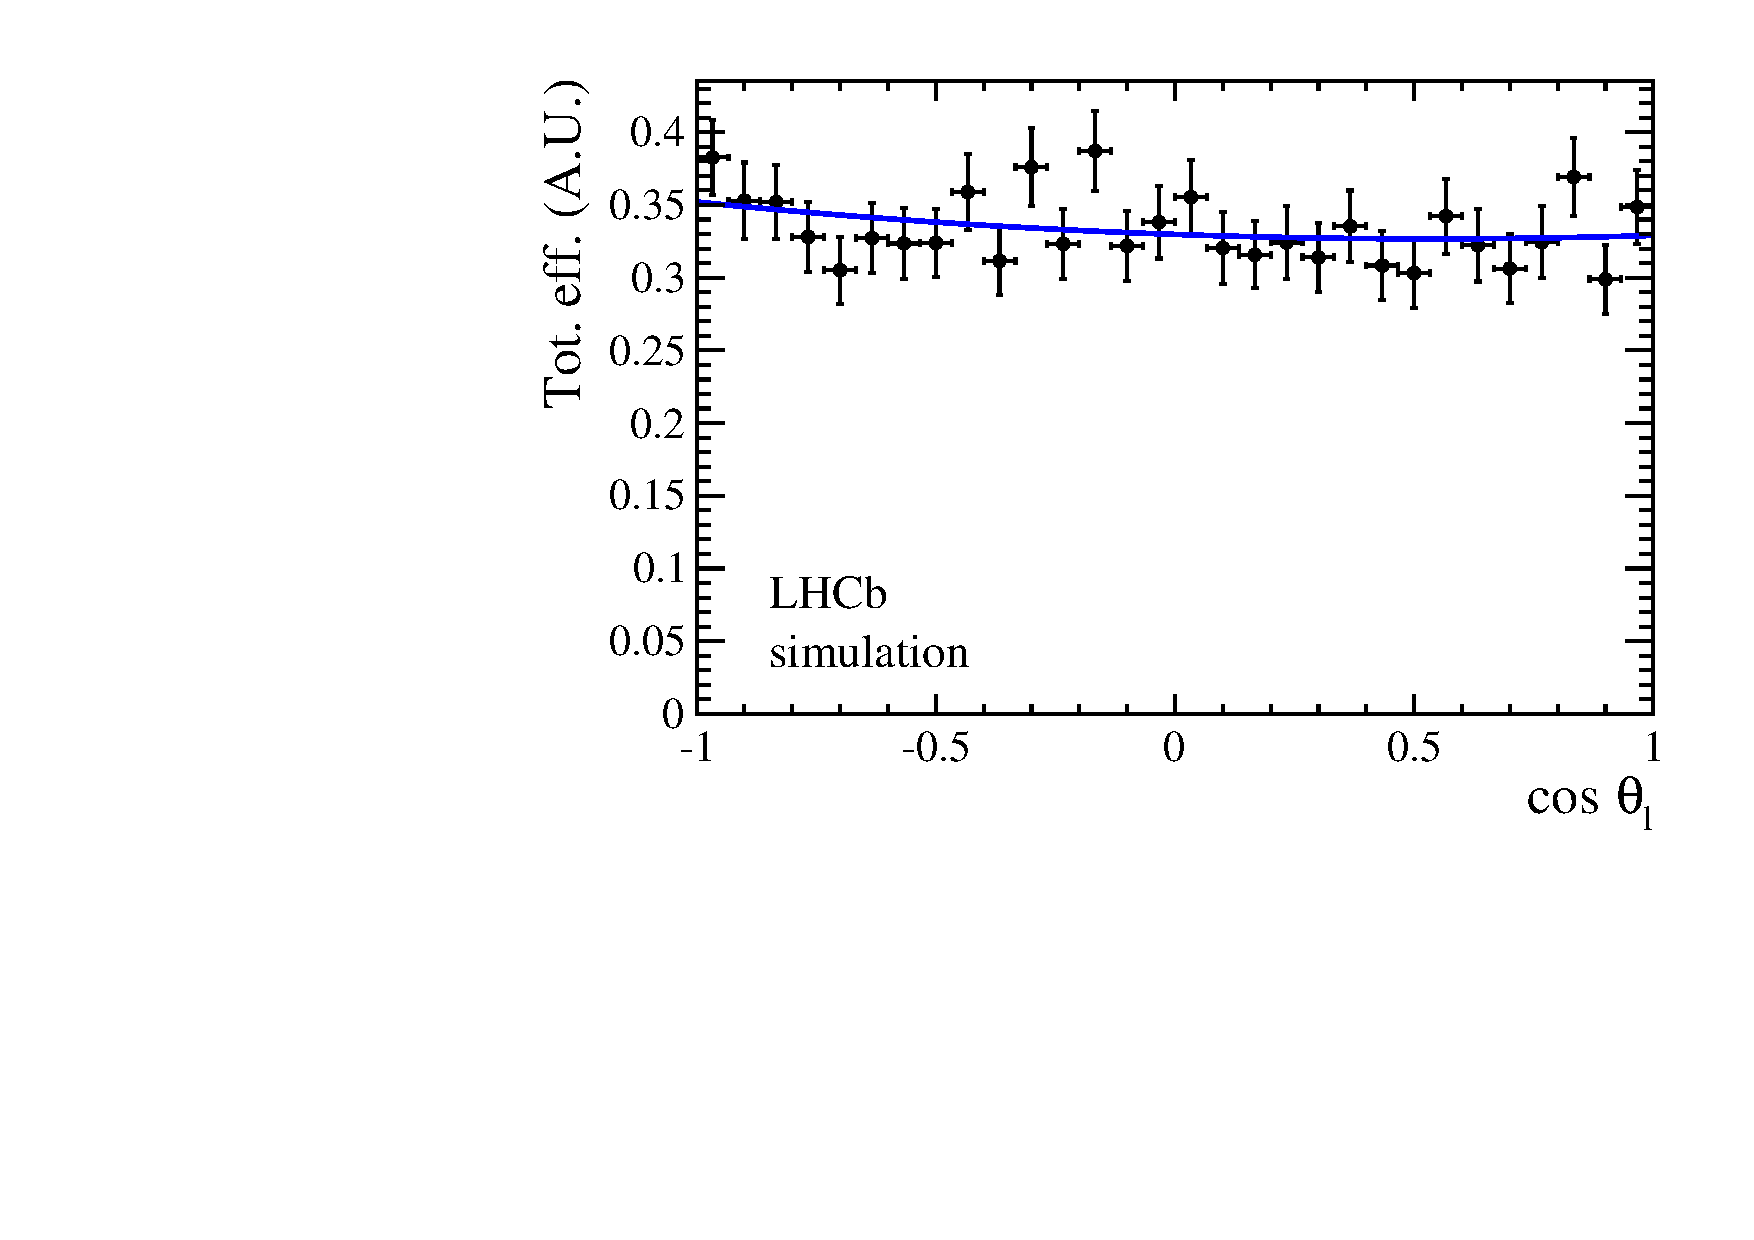
\includegraphics[width=0.48\textwidth]{Lmumu/figs/efficiencies/angular/DDeffFit_q2_1500_2000.pdf}
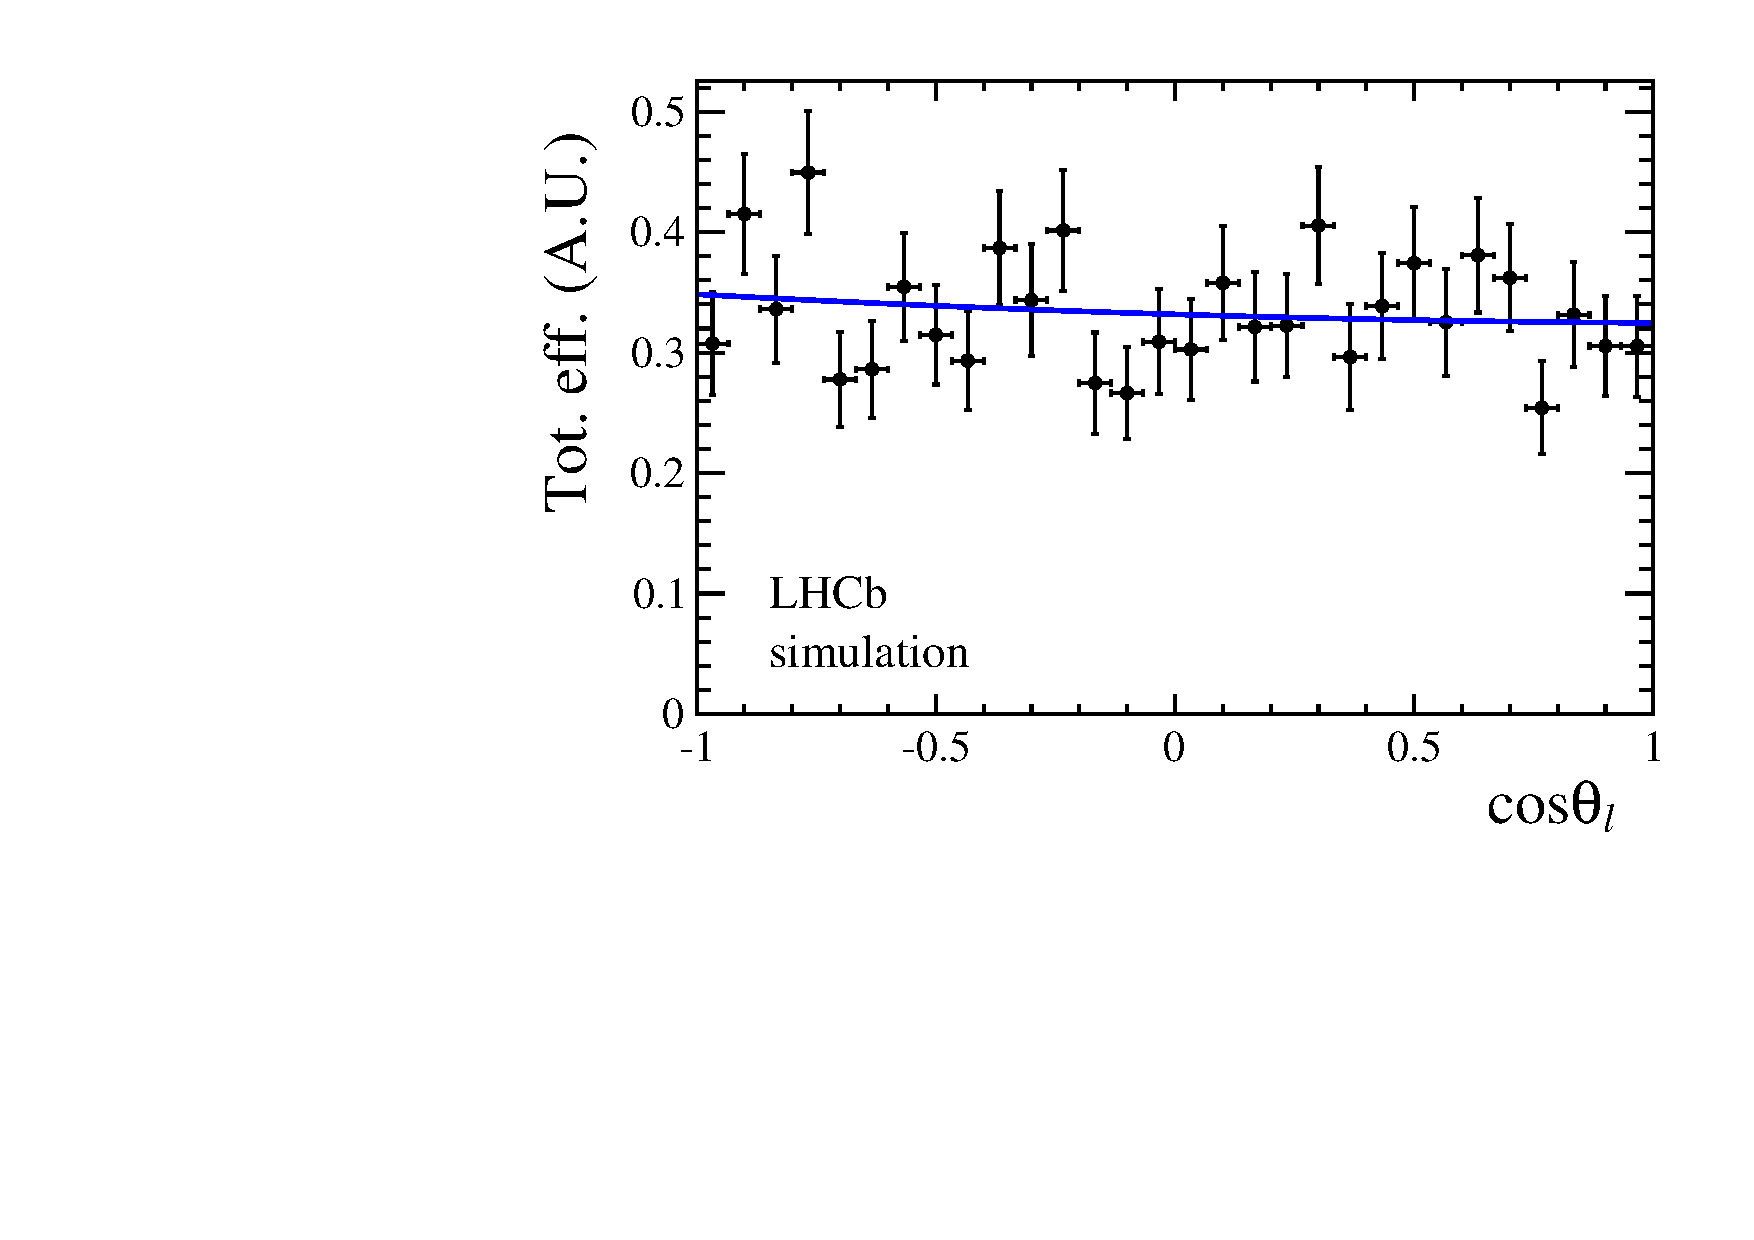
\includegraphics[width=0.48\textwidth]{Lmumu/figs/efficiencies/angular/LLeffFit_q2_1500_2000.pdf}
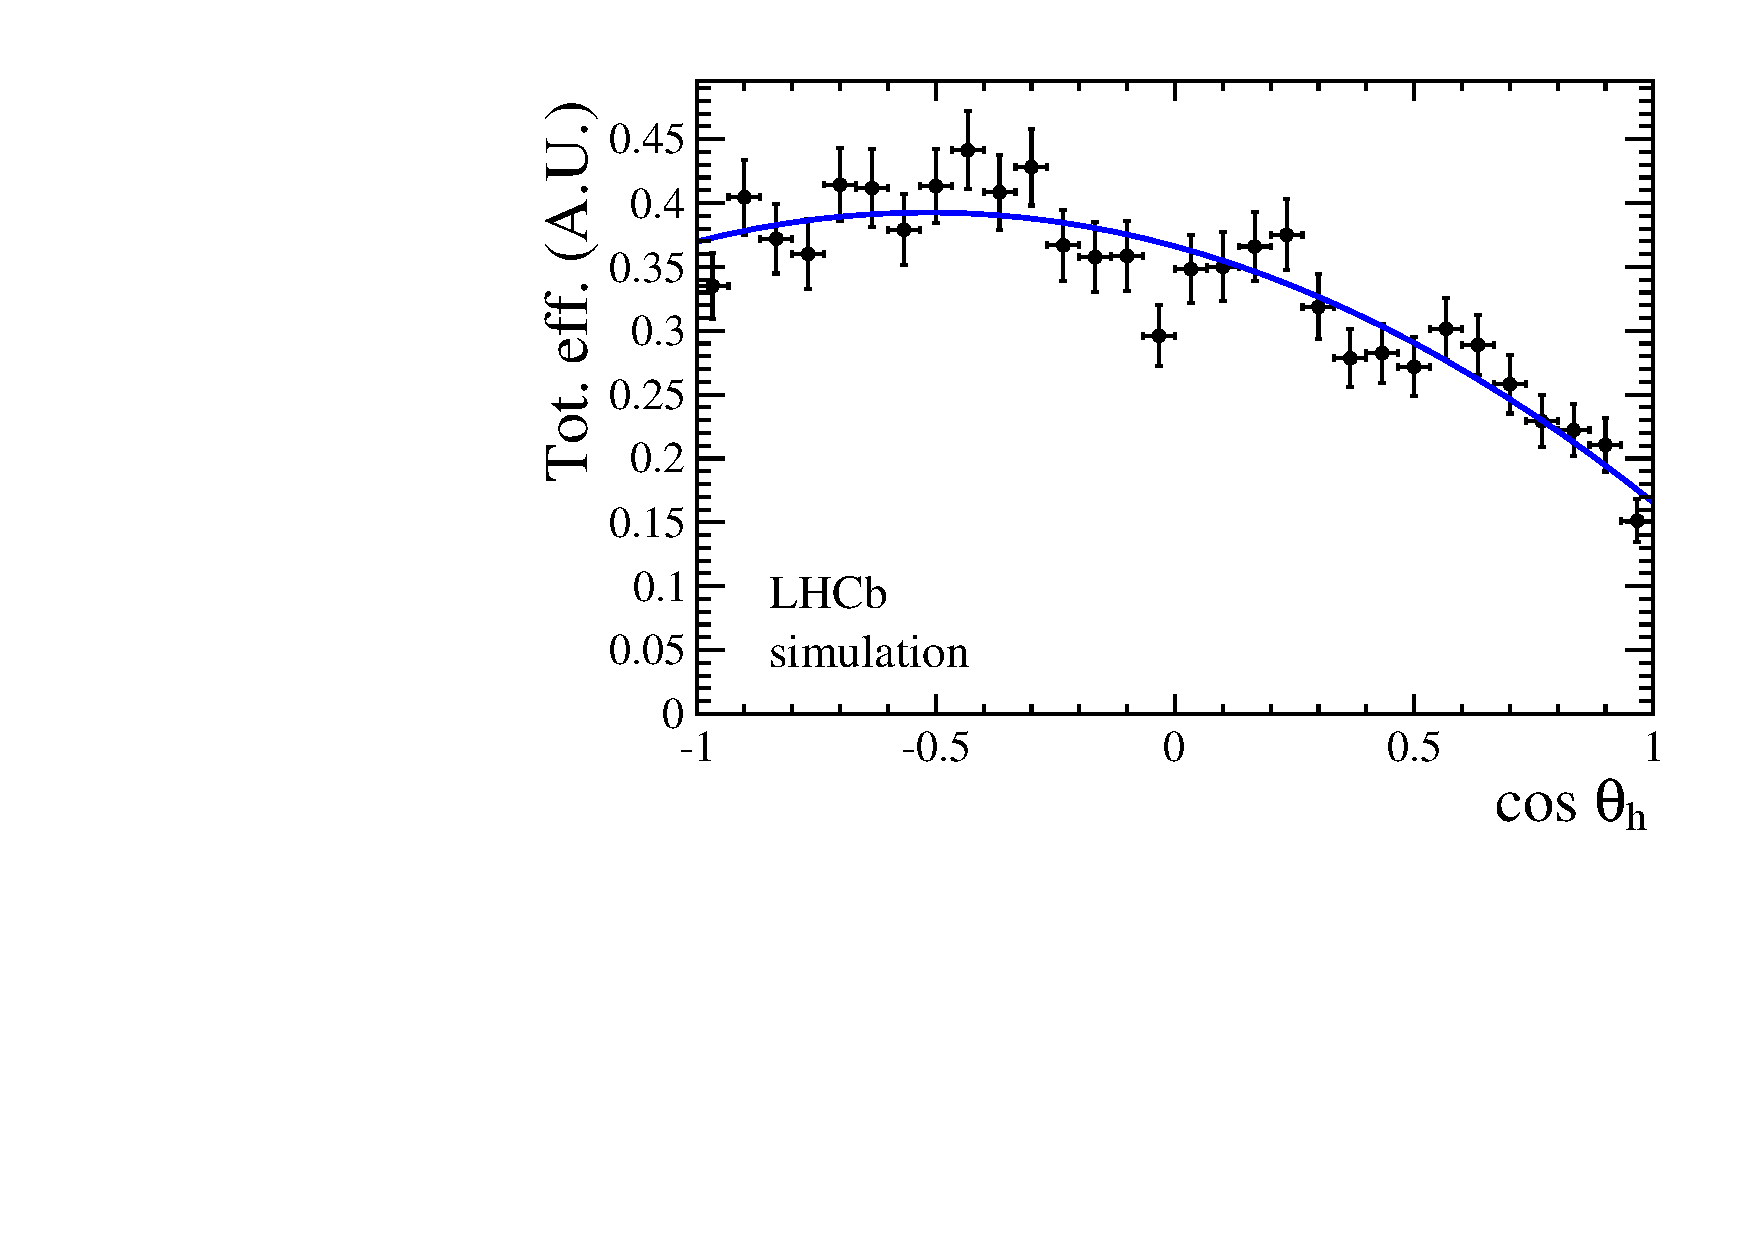
\includegraphics[width=0.48\textwidth]{Lmumu/figs/efficiencies/angular/DDeffFitB_q2_1500_2000.pdf}
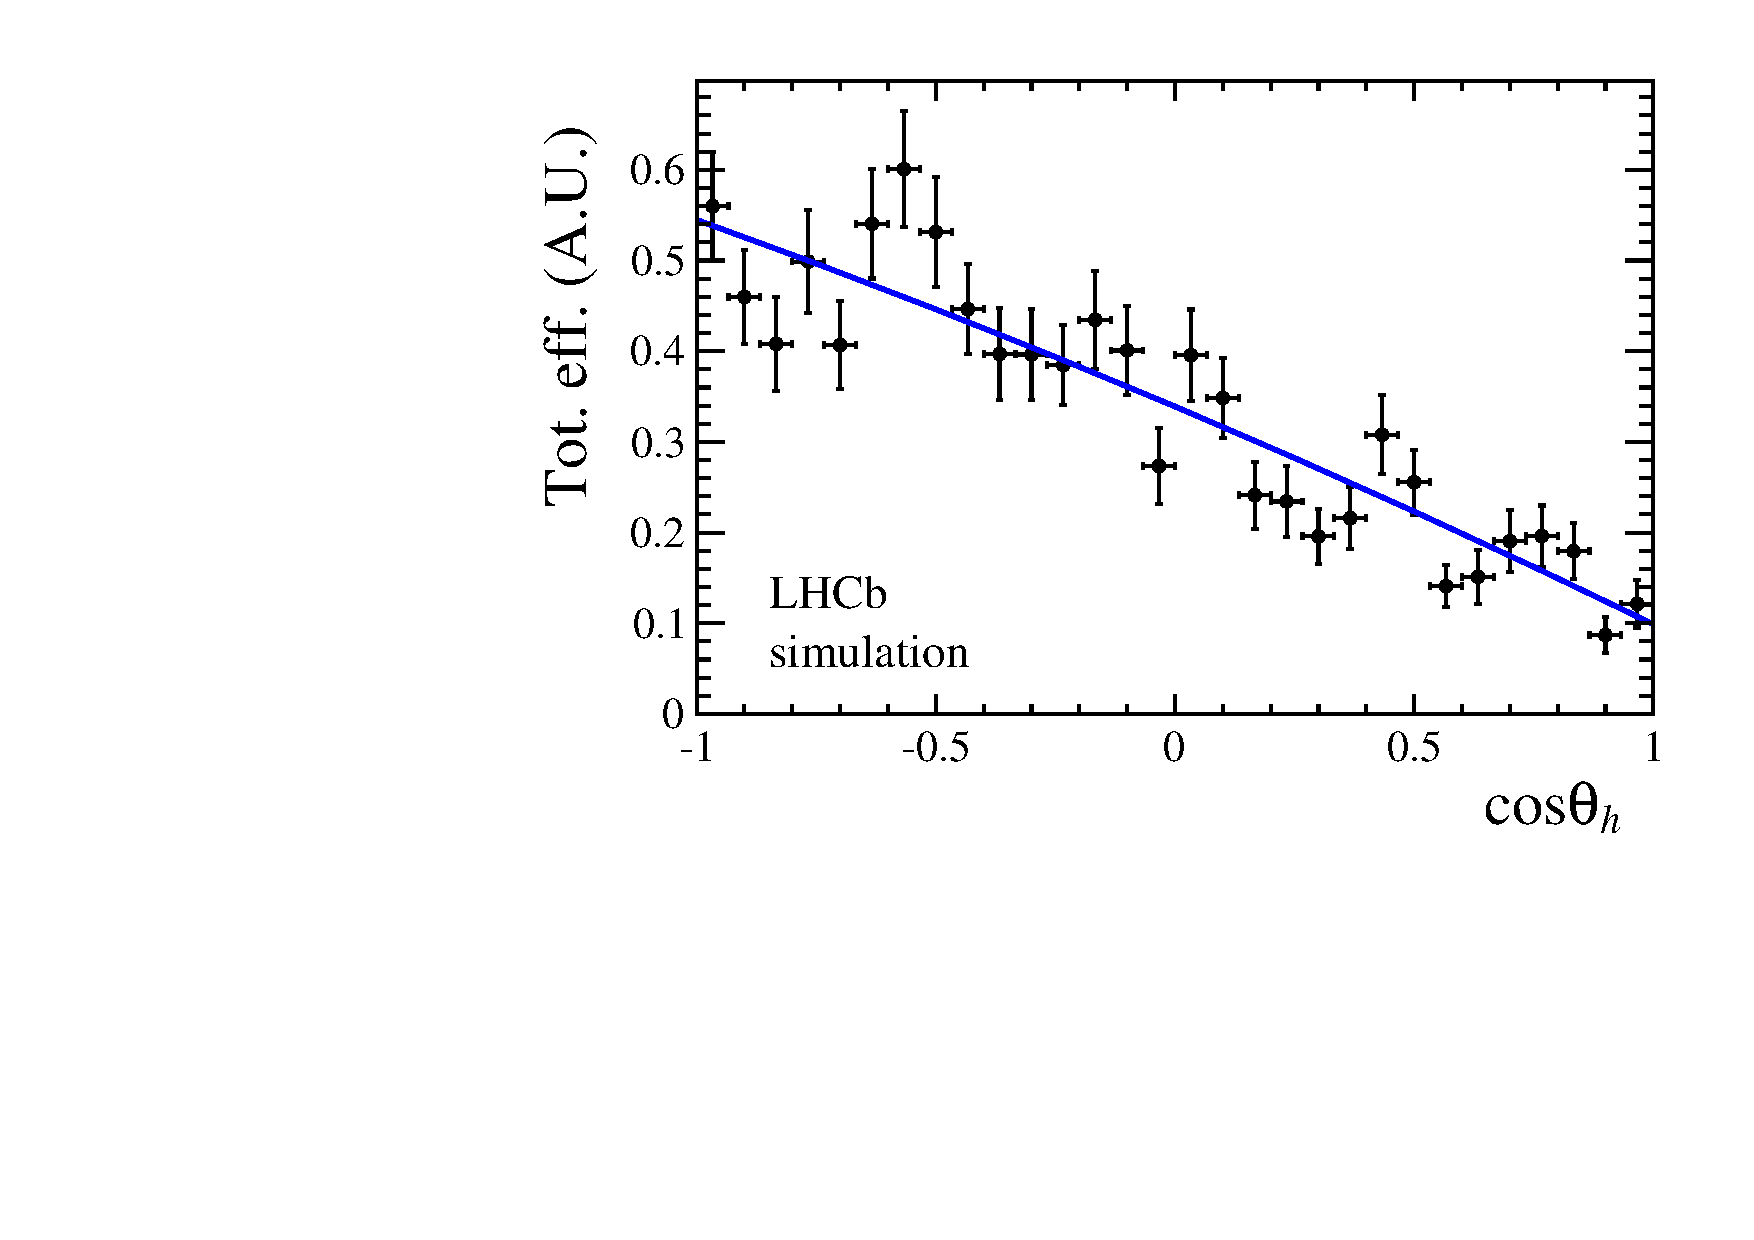
\includegraphics[width=0.48\textwidth]{Lmumu/figs/efficiencies/angular/LLeffFitB_q2_1500_2000.pdf}
\caption{Efficiency as a function of $\cos\theta_\ell$ (top) and $\cos\theta_h$ (bottom) for
downstream (left) and long (right) candidates in the 15--20 \gevgevcccc ~\qsq interval.  }
\label{fig:angular_eff}
\end{figure}
%
%\begin{figure}[h]
%\centering
%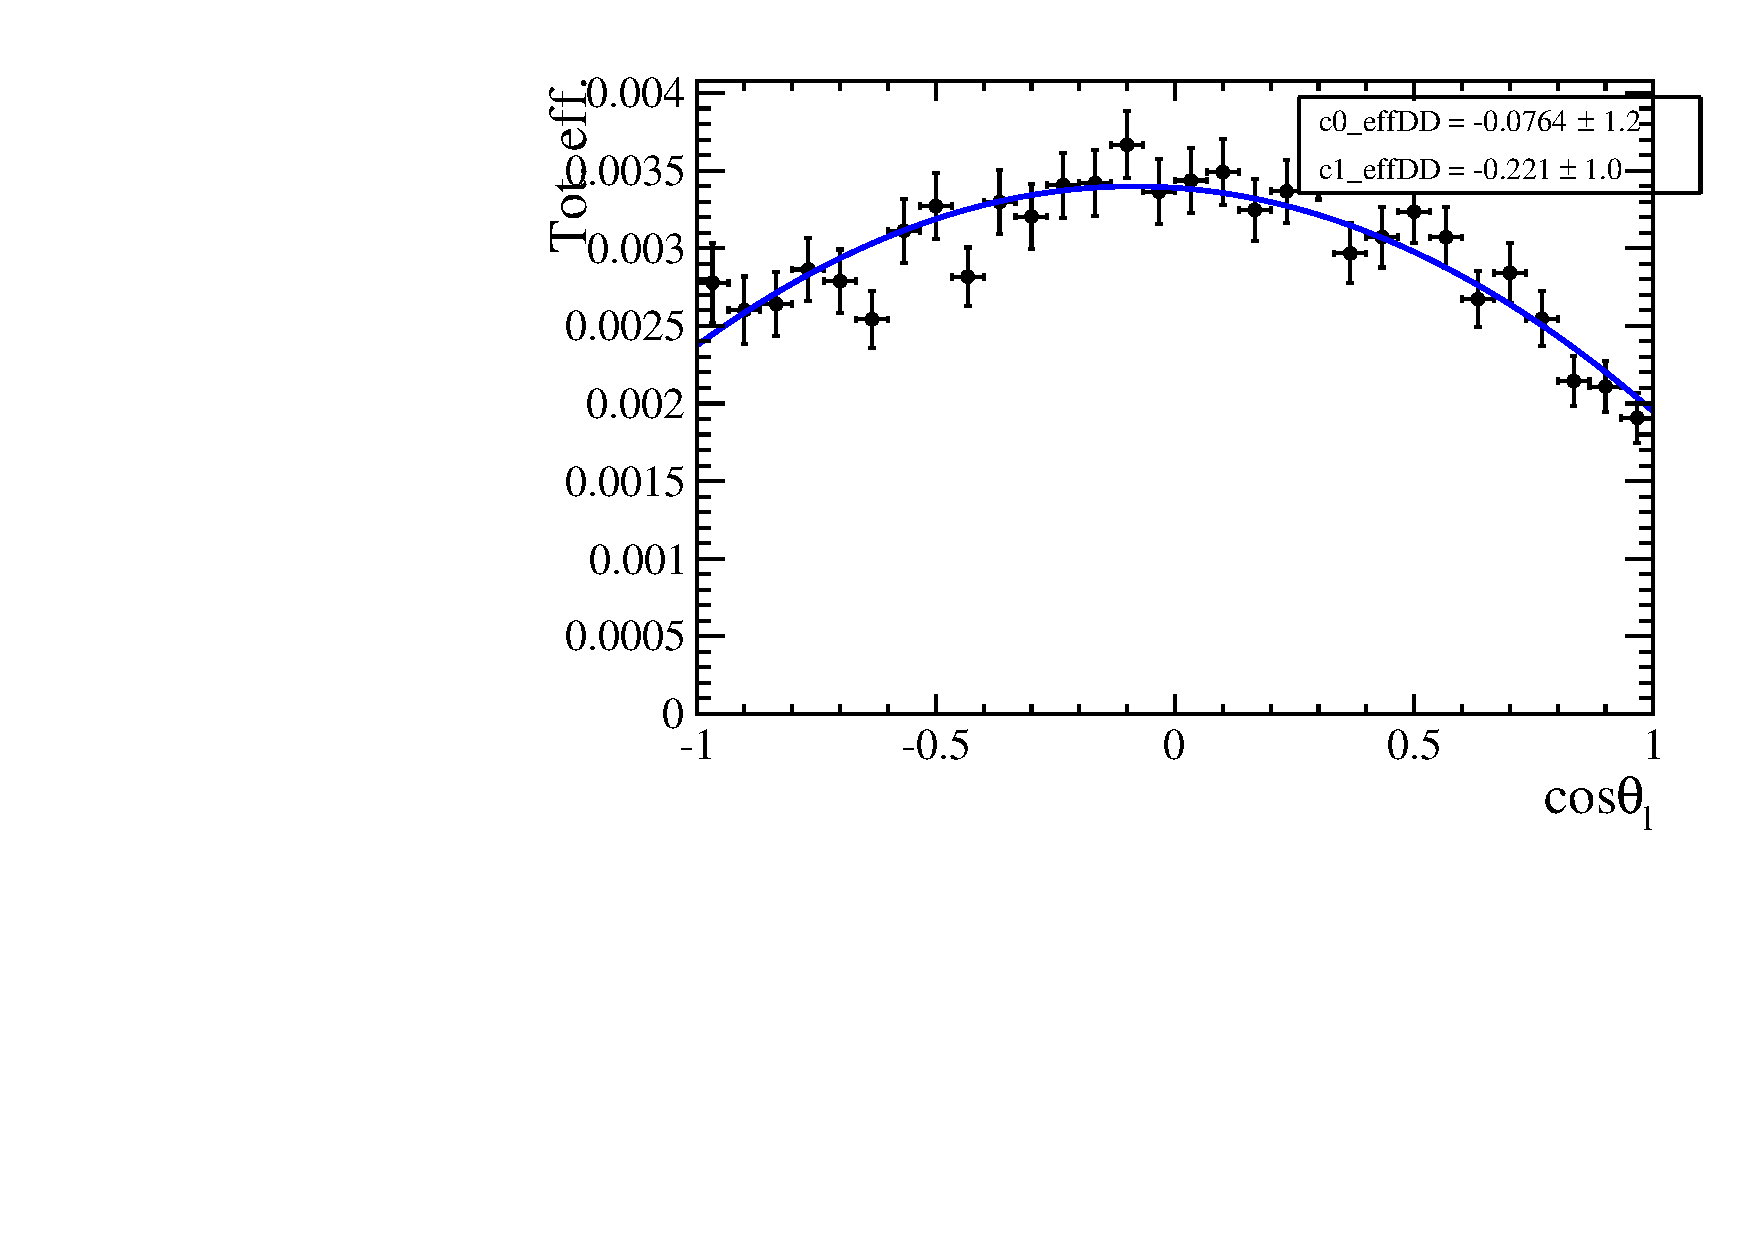
\includegraphics[width=0.48\textwidth]{Lmumu/figs/efficiencies/angular/DDeffFit_q2_110_600.pdf}
%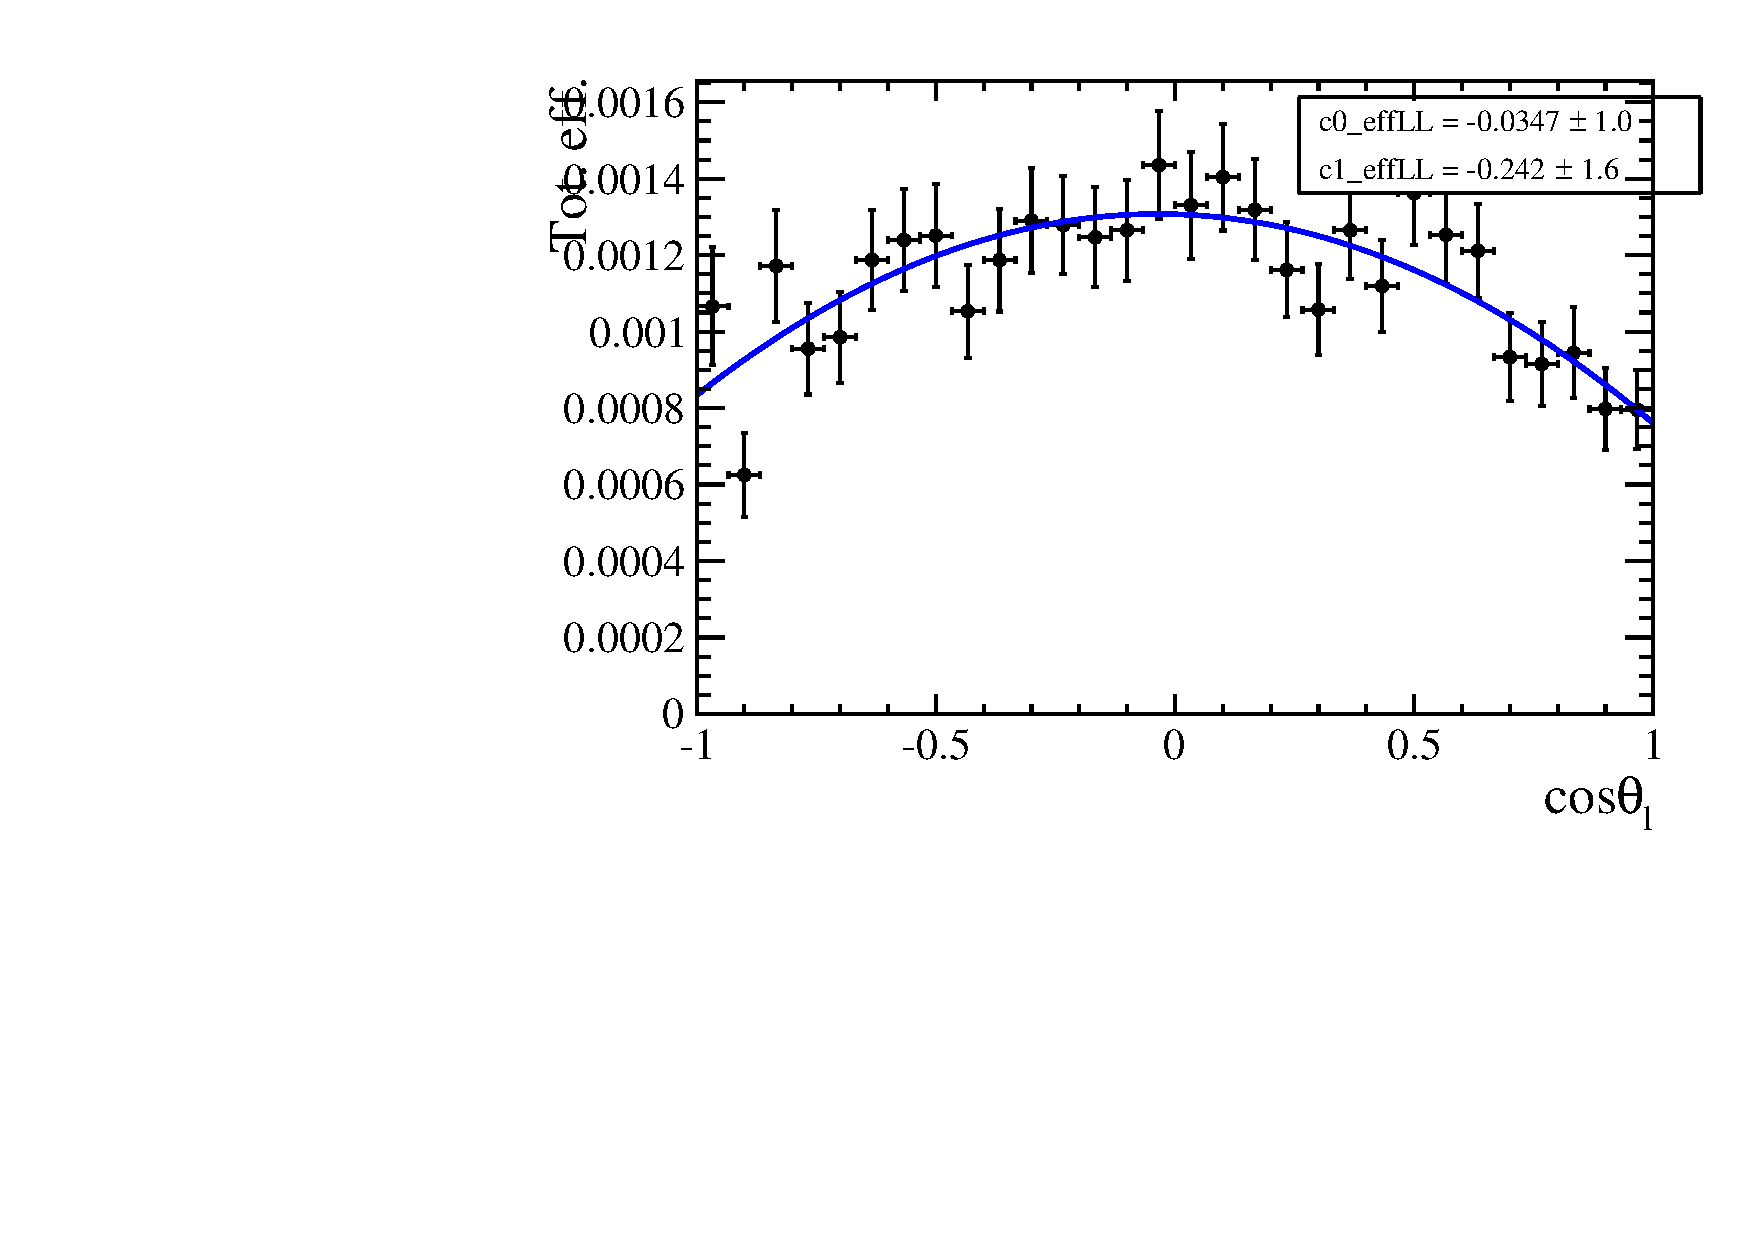
\includegraphics[width=0.48\textwidth]{Lmumu/figs/efficiencies/angular/LLeffFit_q2_110_600.pdf}
%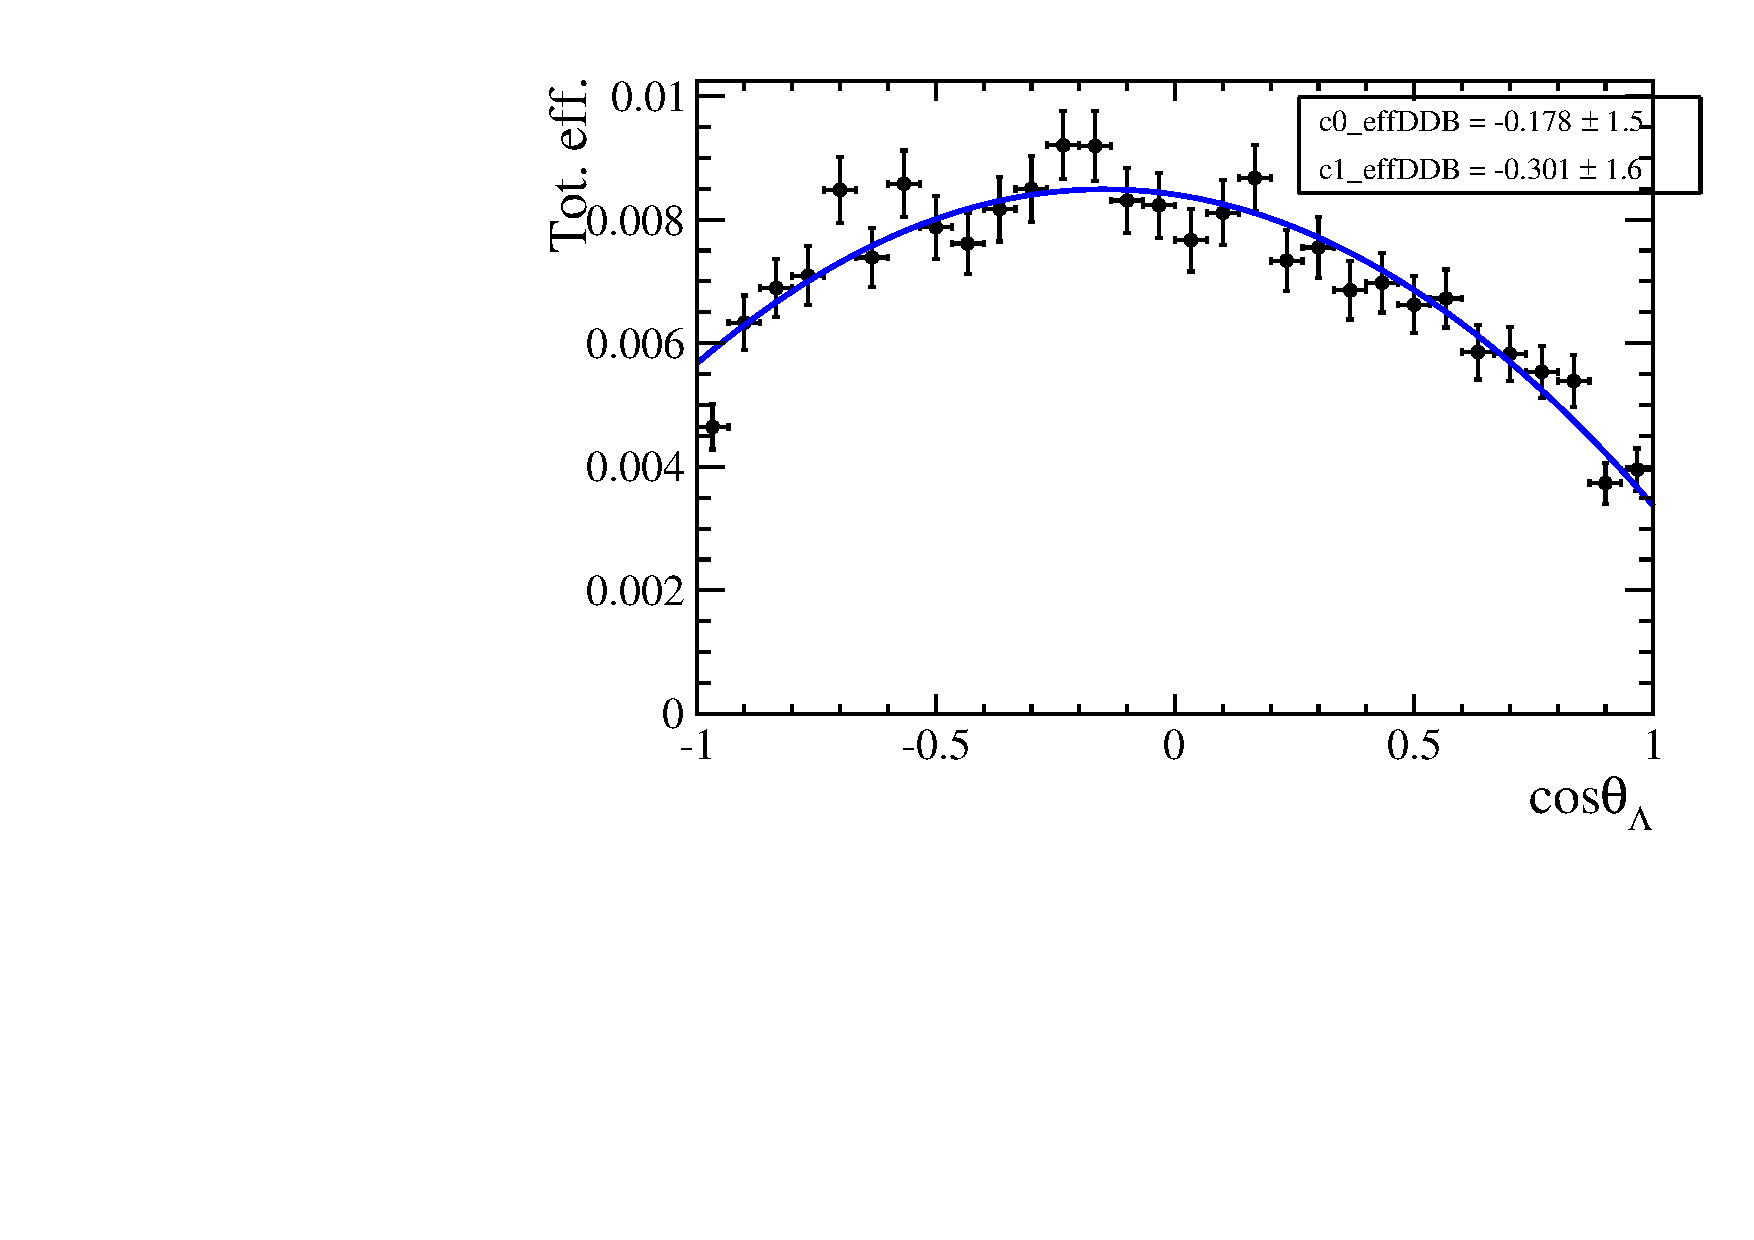
\includegraphics[width=0.48\textwidth]{Lmumu/figs/efficiencies/angular/DDeffFitB_q2_110_600.pdf}
%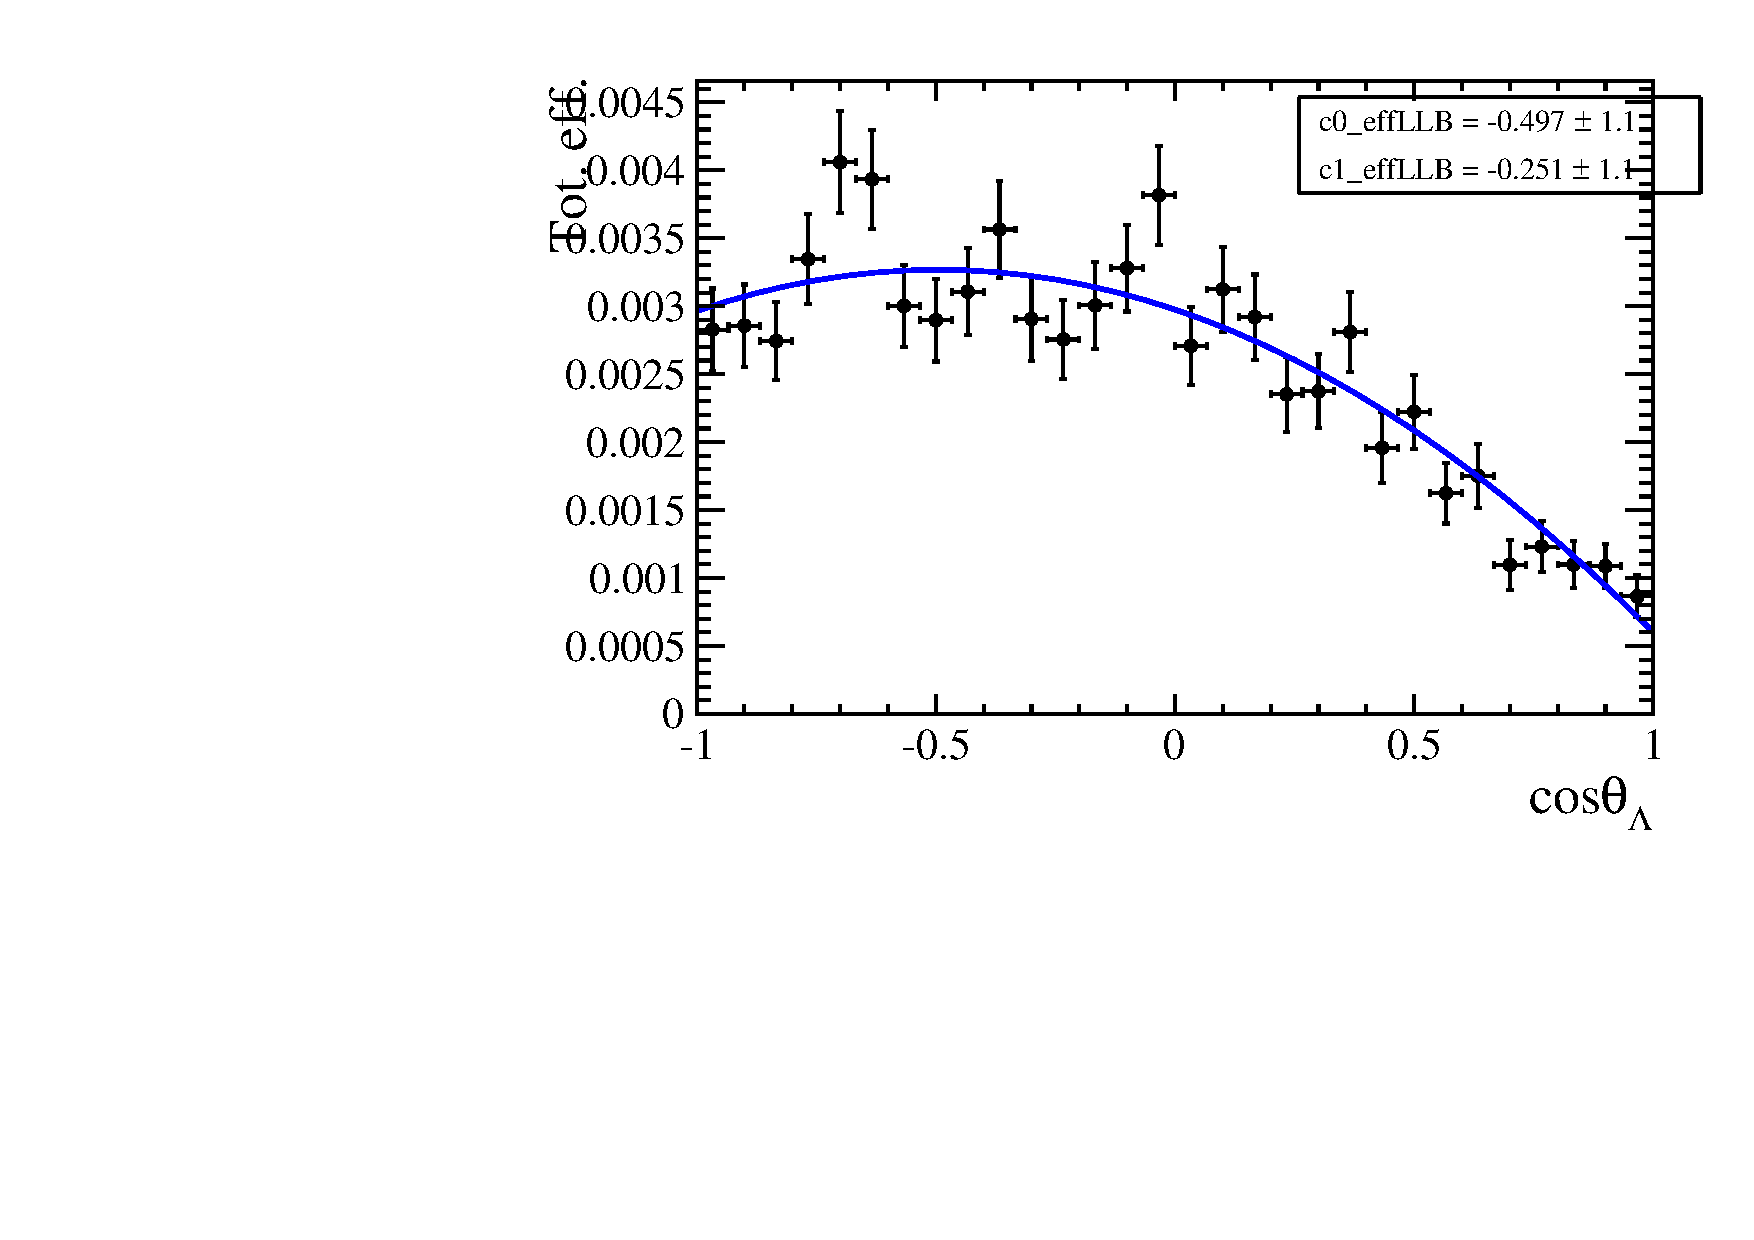
\includegraphics[width=0.48\textwidth]{Lmumu/figs/efficiencies/angular/LLeffFitB_q2_110_600.pdf}
%\caption{Efficiency as a function of $\cos\theta_\ell$ (top) and $\cos\theta_h$ (bottom) for
%downstream (left) and long (right) candidates in the 1.1--6.0 \gevgevcccc ~\qsq interval.  }
%\label{fig:cosThetaBeffLow}
%\end{figure}
%
%\begin{figure}[h]
%\centering
%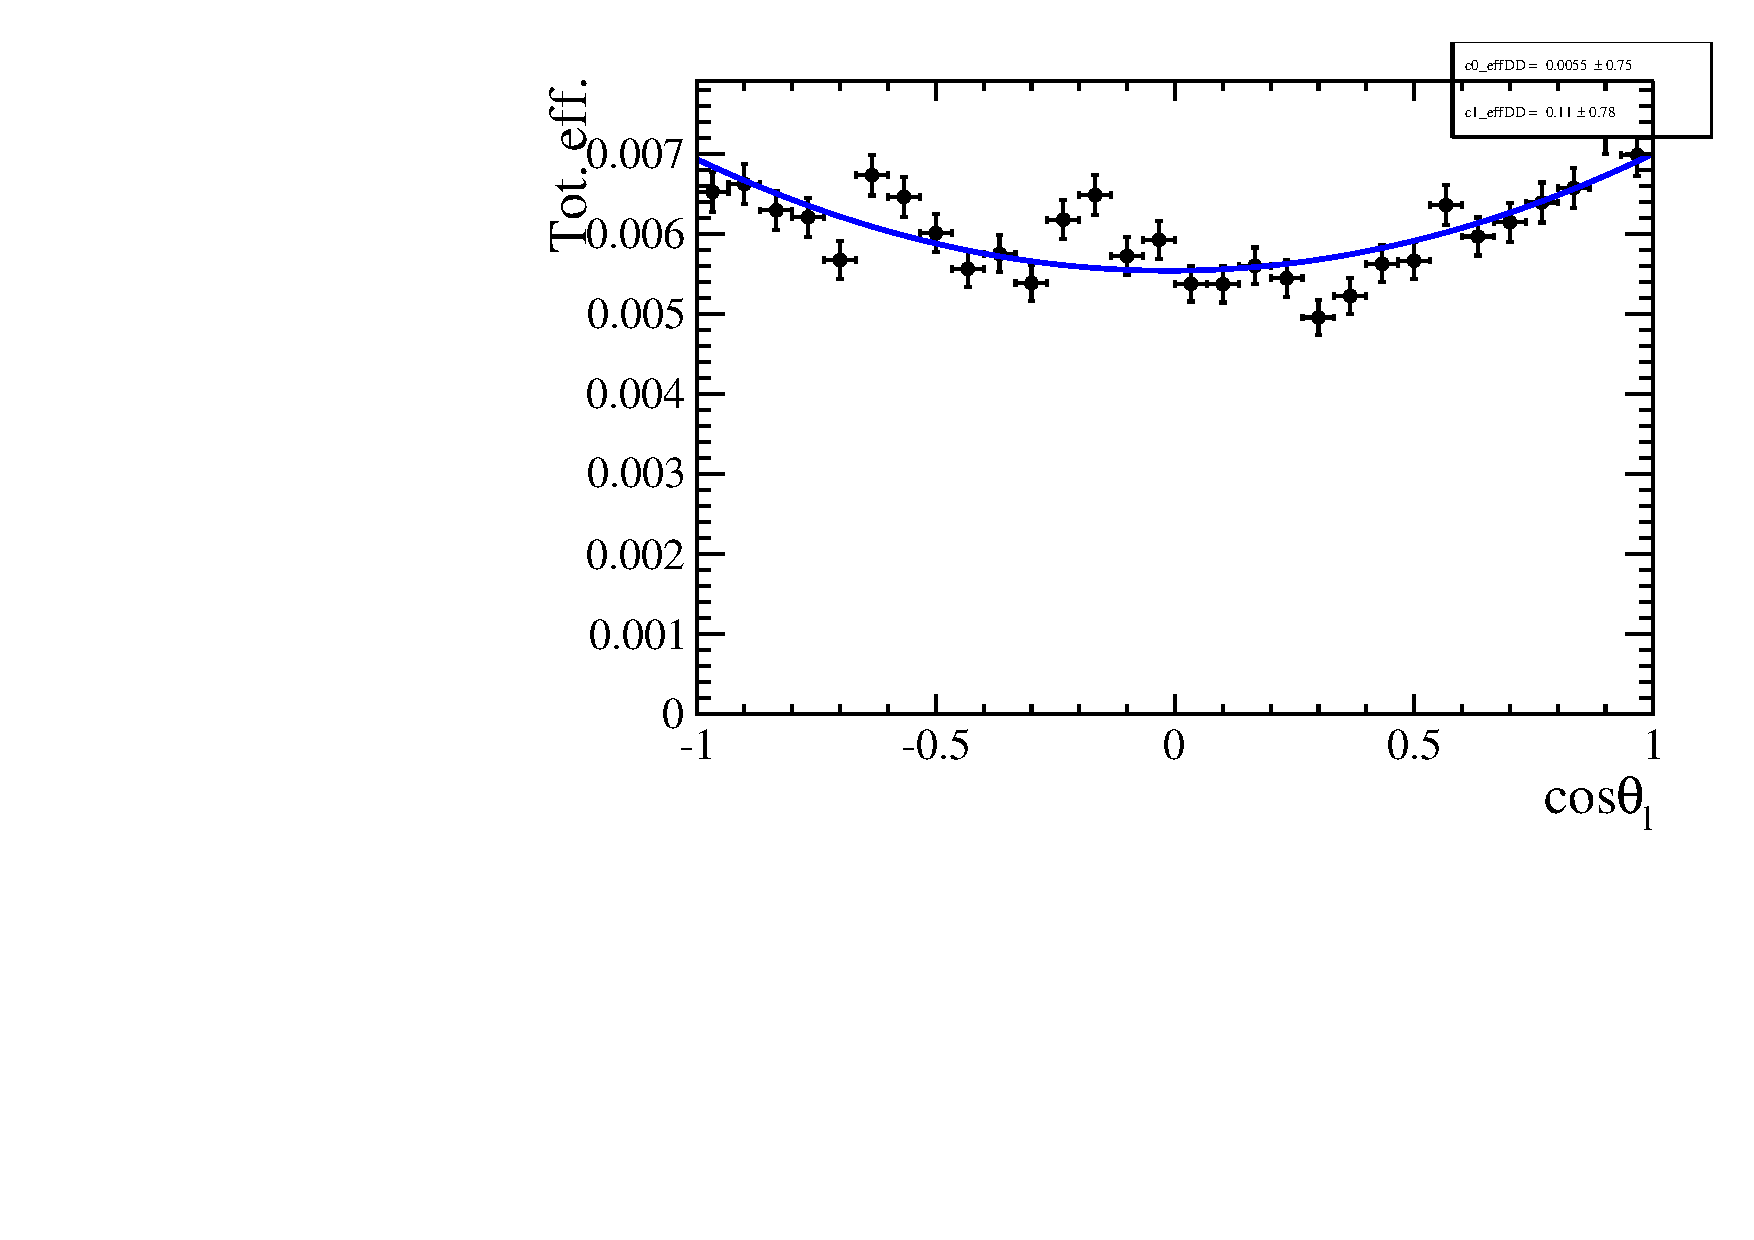
\includegraphics[width=0.45\textwidth]{Lmumu/figs/efficiencies/angular/DDeffFit_jpsi.pdf}
%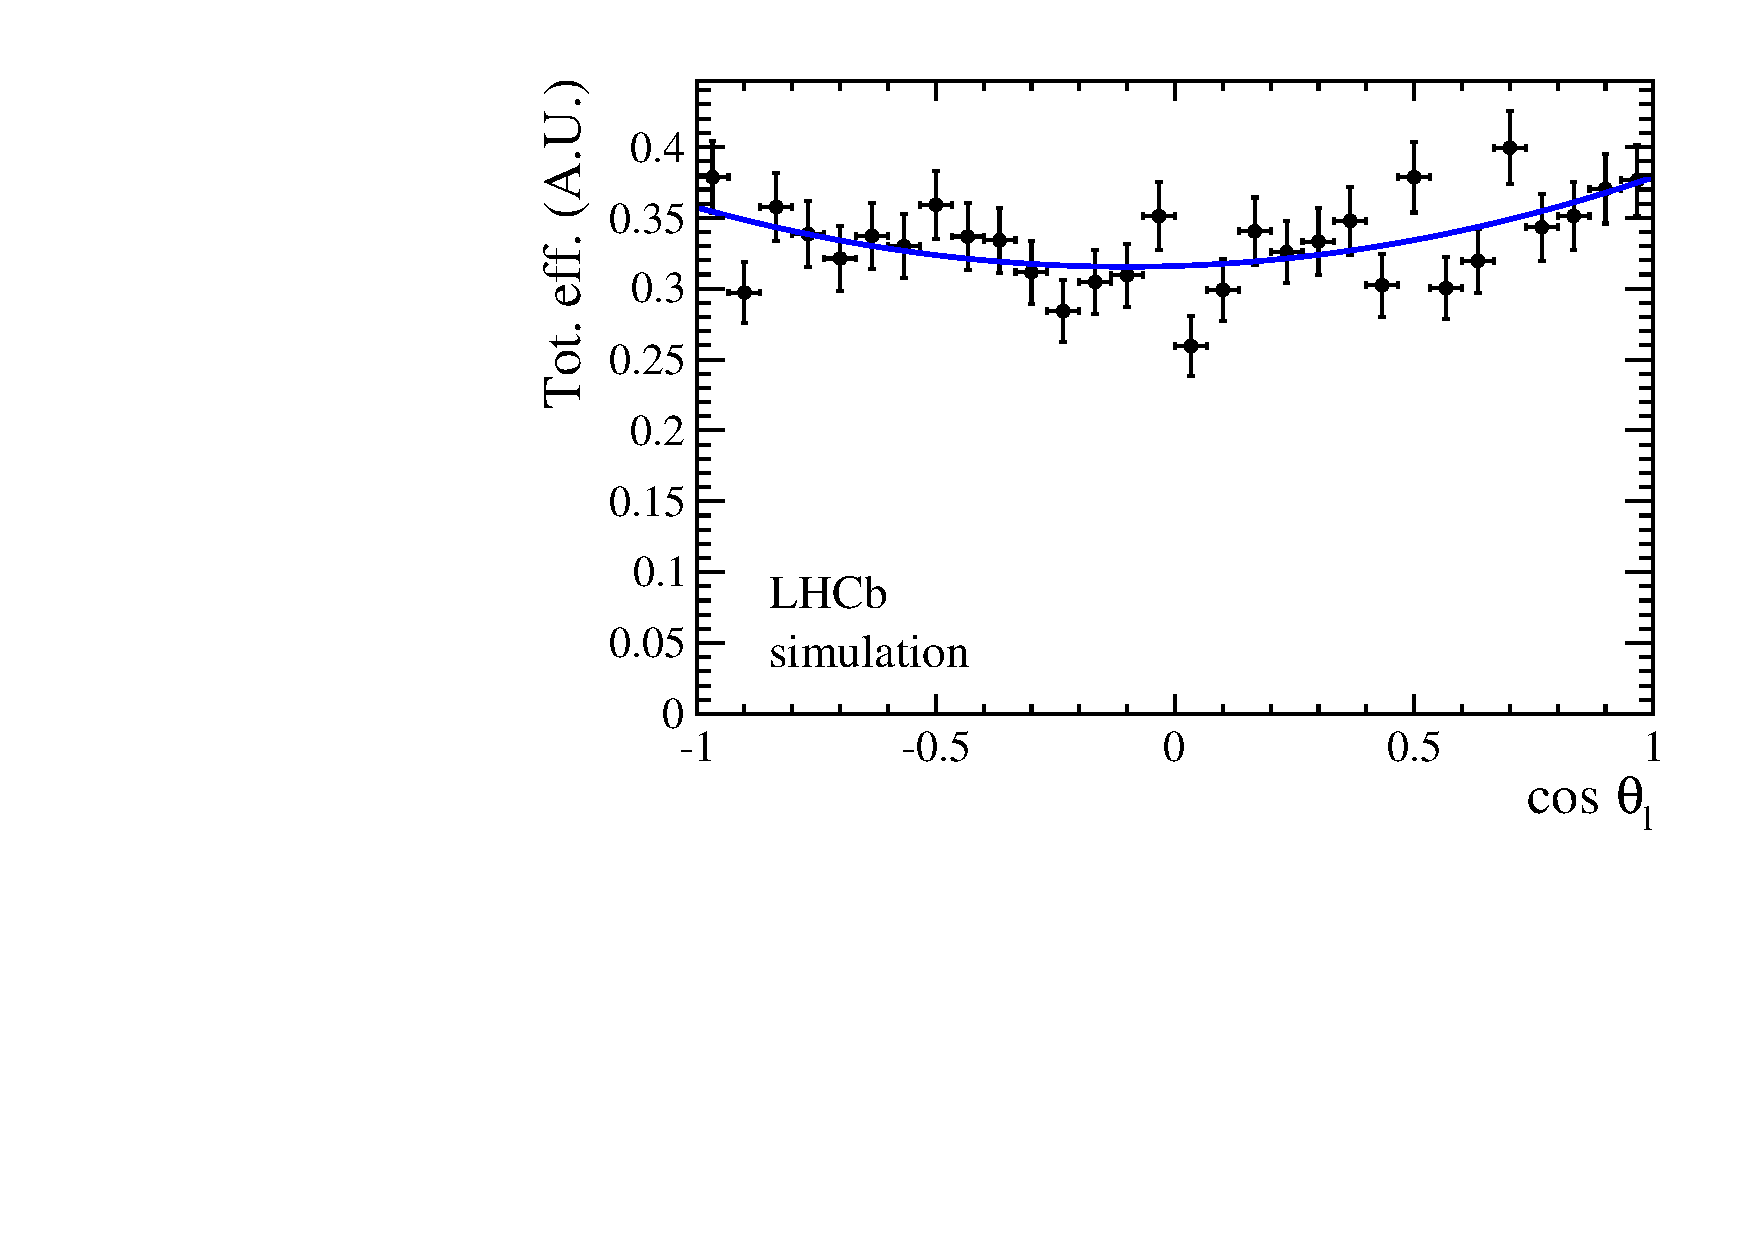
\includegraphics[width=0.45\textwidth]{Lmumu/figs/efficiencies/angular/LLeffFit_jpsi.pdf}
%\caption{Efficiency as a function of $\cos\theta_\ell$ for down-down (left) and long-long (right) events for $J/\psi$ events.  }
%\label{fig:cosThetaLeffJpsi}
%\end{figure}
%
%\begin{figure}[h]
%\centering
%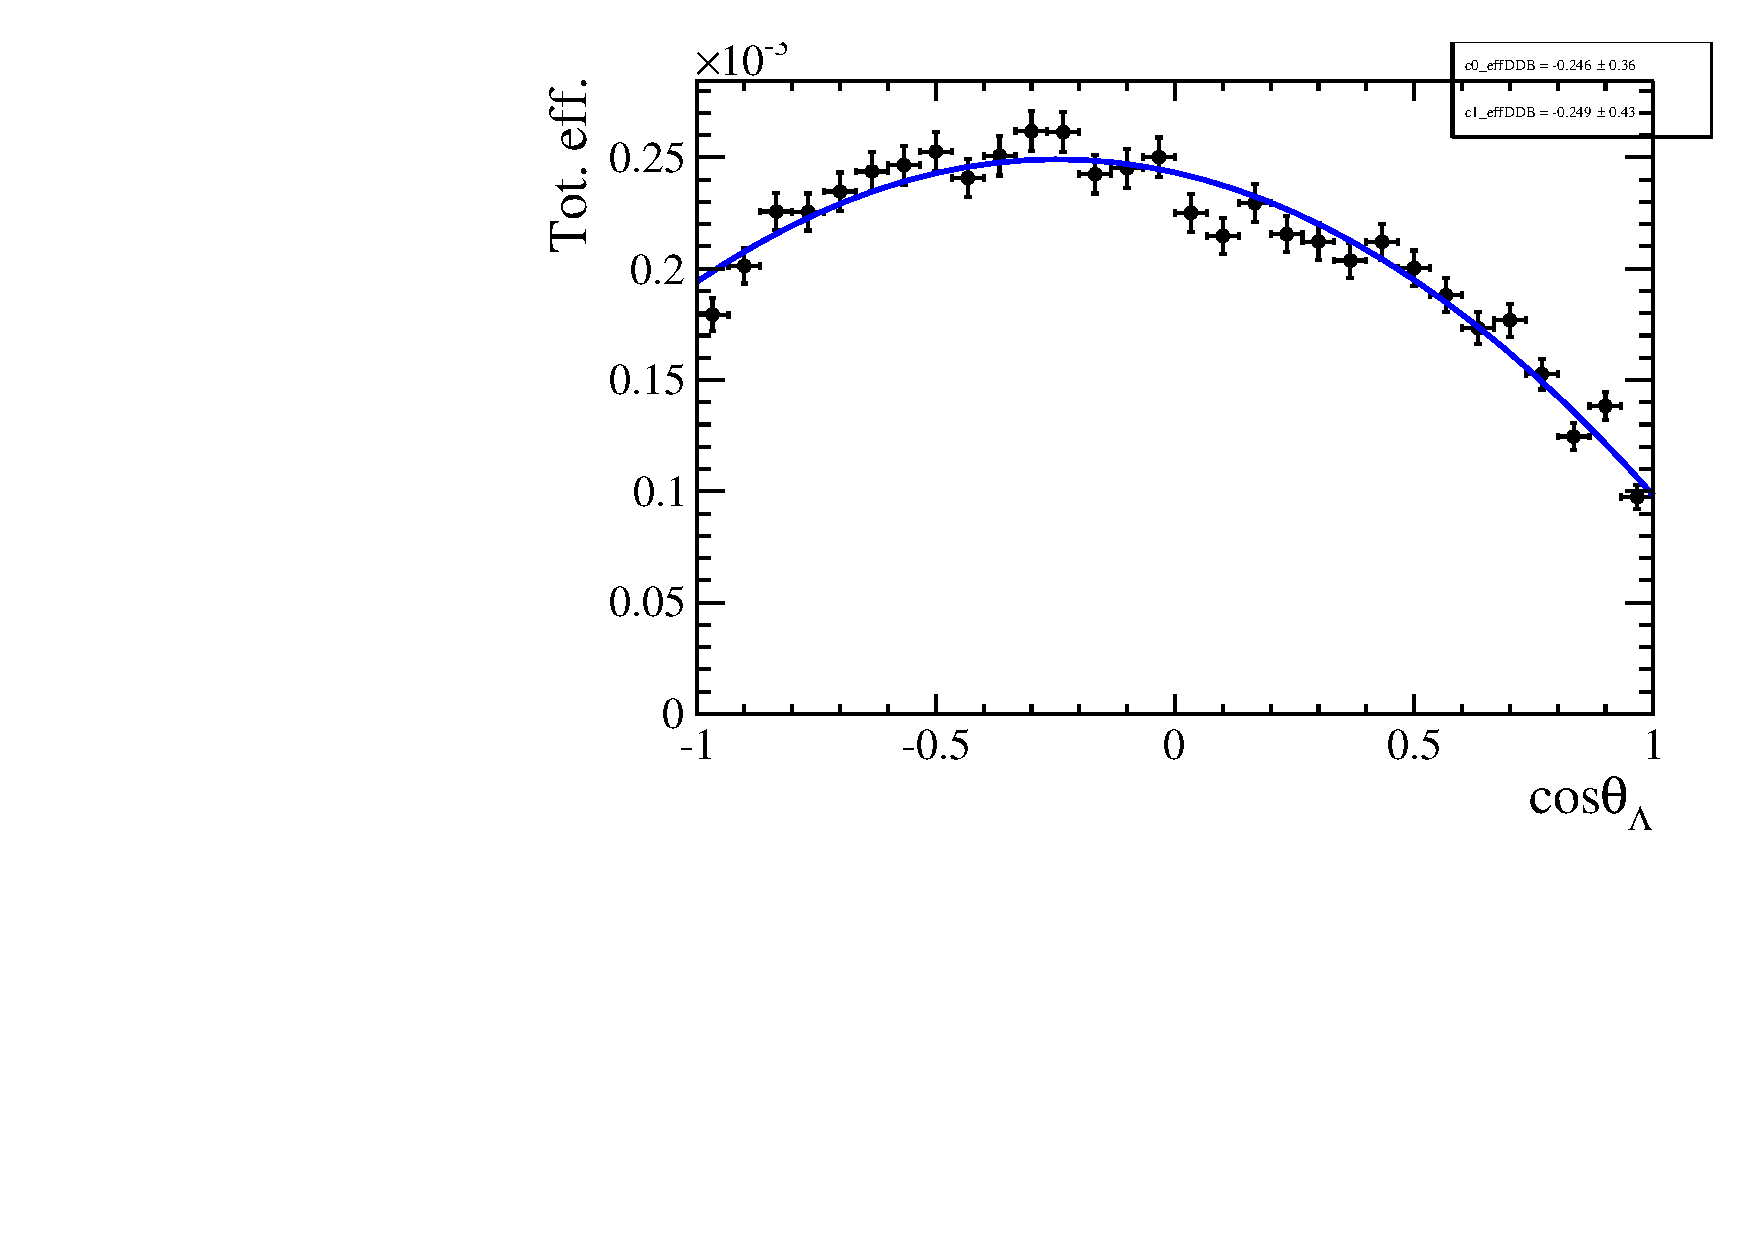
\includegraphics[width=0.45\textwidth]{Lmumu/figs/efficiencies/angular/DDeffFitB_jpsi.pdf}
%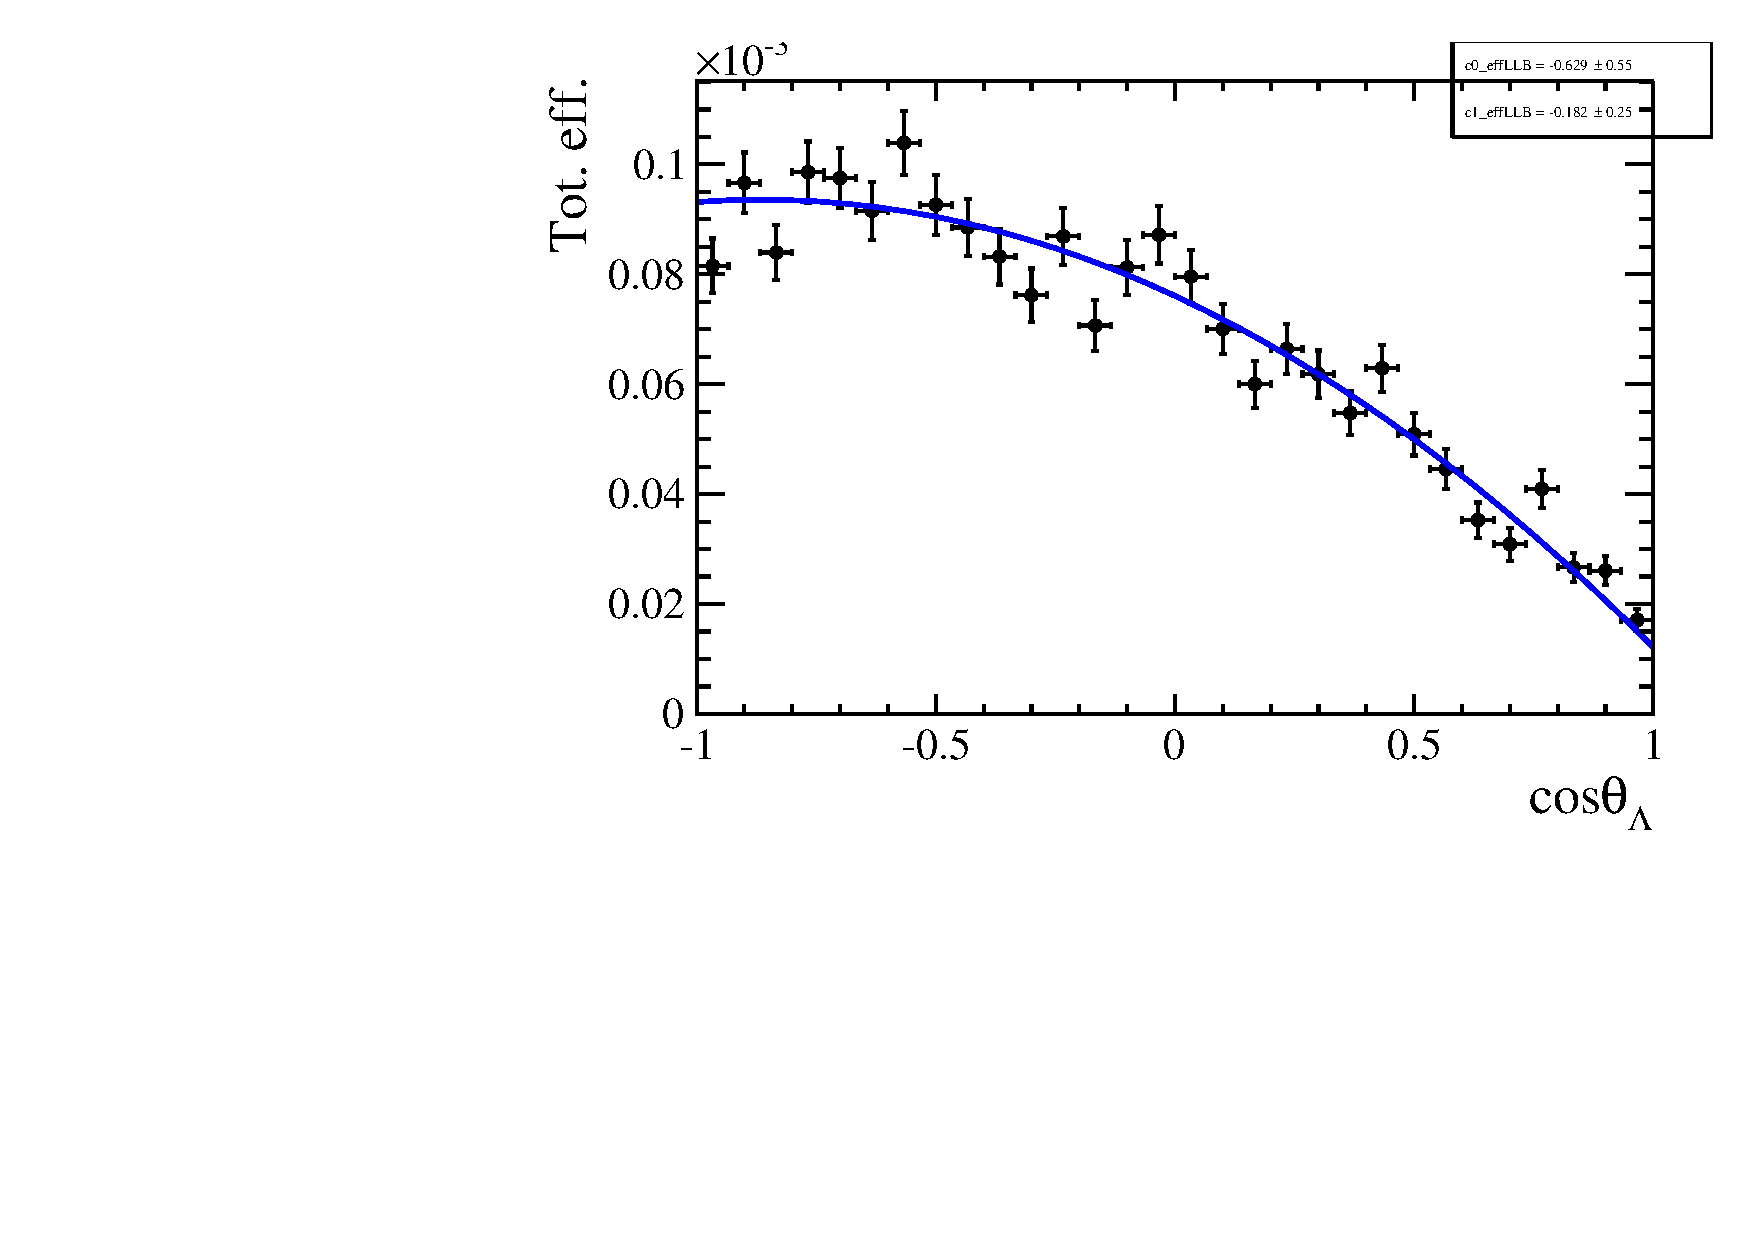
\includegraphics[width=0.45\textwidth]{Lmumu/figs/efficiencies/angular/LLeffFitB_jpsi.pdf}
%\caption{Efficiency as a function of $\cos\theta_\Lambda$ for down-down (left) and long-long (right) events for $J/\psi$ events.  }
%\label{fig:cosThetaBeffJpsi}
%\end{figure}


%Finally, since fits are performed on one-dimensional projections, this implies an integral over
%the other angular variables. If the efficiency is not flat in these variables we could have extra
%terms left in eq. \ref{eq:afbTh} and \ref{eq:afbLTh}. We take in account for this effect in the 
%systematics as described in the following sections. 

\section{Studies on a three-dimensional fit}

One other way of extracting the angular observables would be to fit at the same time both angles 
and also the invariant mass distribution in order to have a better handle on the level of background.
In this case one can use more of the information available. On the other hand it is necessary to use 
a larger mass window including more background and this method involves more parameters to fit.
In the 1D case the free parameters are the two parameters of interest ($A_{\rm FB}^\ell$ and $f_{\rm L}$)
for the lepton case and one ($A_{\rm FB}^h$)
for the hadron one. For the 3D case the free parameters are the three parameters of interest 
plus two background fractions and the two exponential slopes for the invariant mass background.
An high number of free parameters is difficult to constrain with the very limited statistics available.
Furthermore, to take correctly into account correlations 3 more observables enter the fit. 
%Therefore we have a total of 4 free parameters for the lepton case and 3 for hadron case fitting in 1D and 7 free parameters in the 3D fit.
%In both cases we obtain the background fractions fitting mass alone and then we gaussian contrain the fractions in the final fit.
%
To check which method gives the best sensitivity 500 pseudo-experiments are generated.
Events are generated in a 3D ($\cos\theta_\ell$,$\cos\theta_h$,m) space using shapes taken from the fit on real data.
The generated values of the parameters of interest are $A_{\rm FB}^\ell = 0$, $f_{\rm L} = 0.7$ 
and $A_{\rm FB}^h = -0.37$. These are data-like values inspired to a preliminary measurement
in the highest statistics interval. The overall statistics and the fraction of background events in the mass
window are generated using the values found from the 1D fit on data.
%This is done using the statistics of our highest statistics bin, $15-20$ $GeV^2/c^2$ in \qsq, 
%and our lowest statistics unblinded bin, $11-12.5$ $GeV^2/c^2$ in \qsq.
Each pseudo-experiment is fitted with both methods and Fig.~\ref{fig:3DtoyResults} reports 
distributions of parameters of interest obtained from the fit in the 1D and 3D cases.
The RMS of these distributions can be taken as a measure of the sensitivity of each method.
In Tab.~\ref{tab:3DtoyResults} RMSs from both methods can be compared. For all parameters 
of interest the 1D fit method gives a smaller RMS, hence a better sensitivity.
%
\begin{table}
\centering
\caption{RMS values for toy experiments on the extraction of the three parameters
of inetersts with the 1D or 3D fitting methods.}
\begin{tabular}{lcccc} \hline
\qsq [\gevgevcccc]         &   Fit type 	 & $A_{\rm FB}^h$  &  $A_{\rm FB}^\ell$ &   $f_{\rm L}$ 	 \\
\hline

\multirow{2}{*}{15.0--20.0} & 1D           &  0.070    &  0.055       &   0.099  \\
			    	       & 3D           &  0.092    &  0.095       &   0.153  \\
\hline
\multirow{2}{*}{11.0--12.5} & 1D           &  0.142    &  0.128       &   0.198  \\
					       & 3D           &  0.249    &  0.254       &   0.303  \\

\hline
\end{tabular}
\label{tab:3DtoyResults}
\end{table}

\begin{figure}[h]
\centering
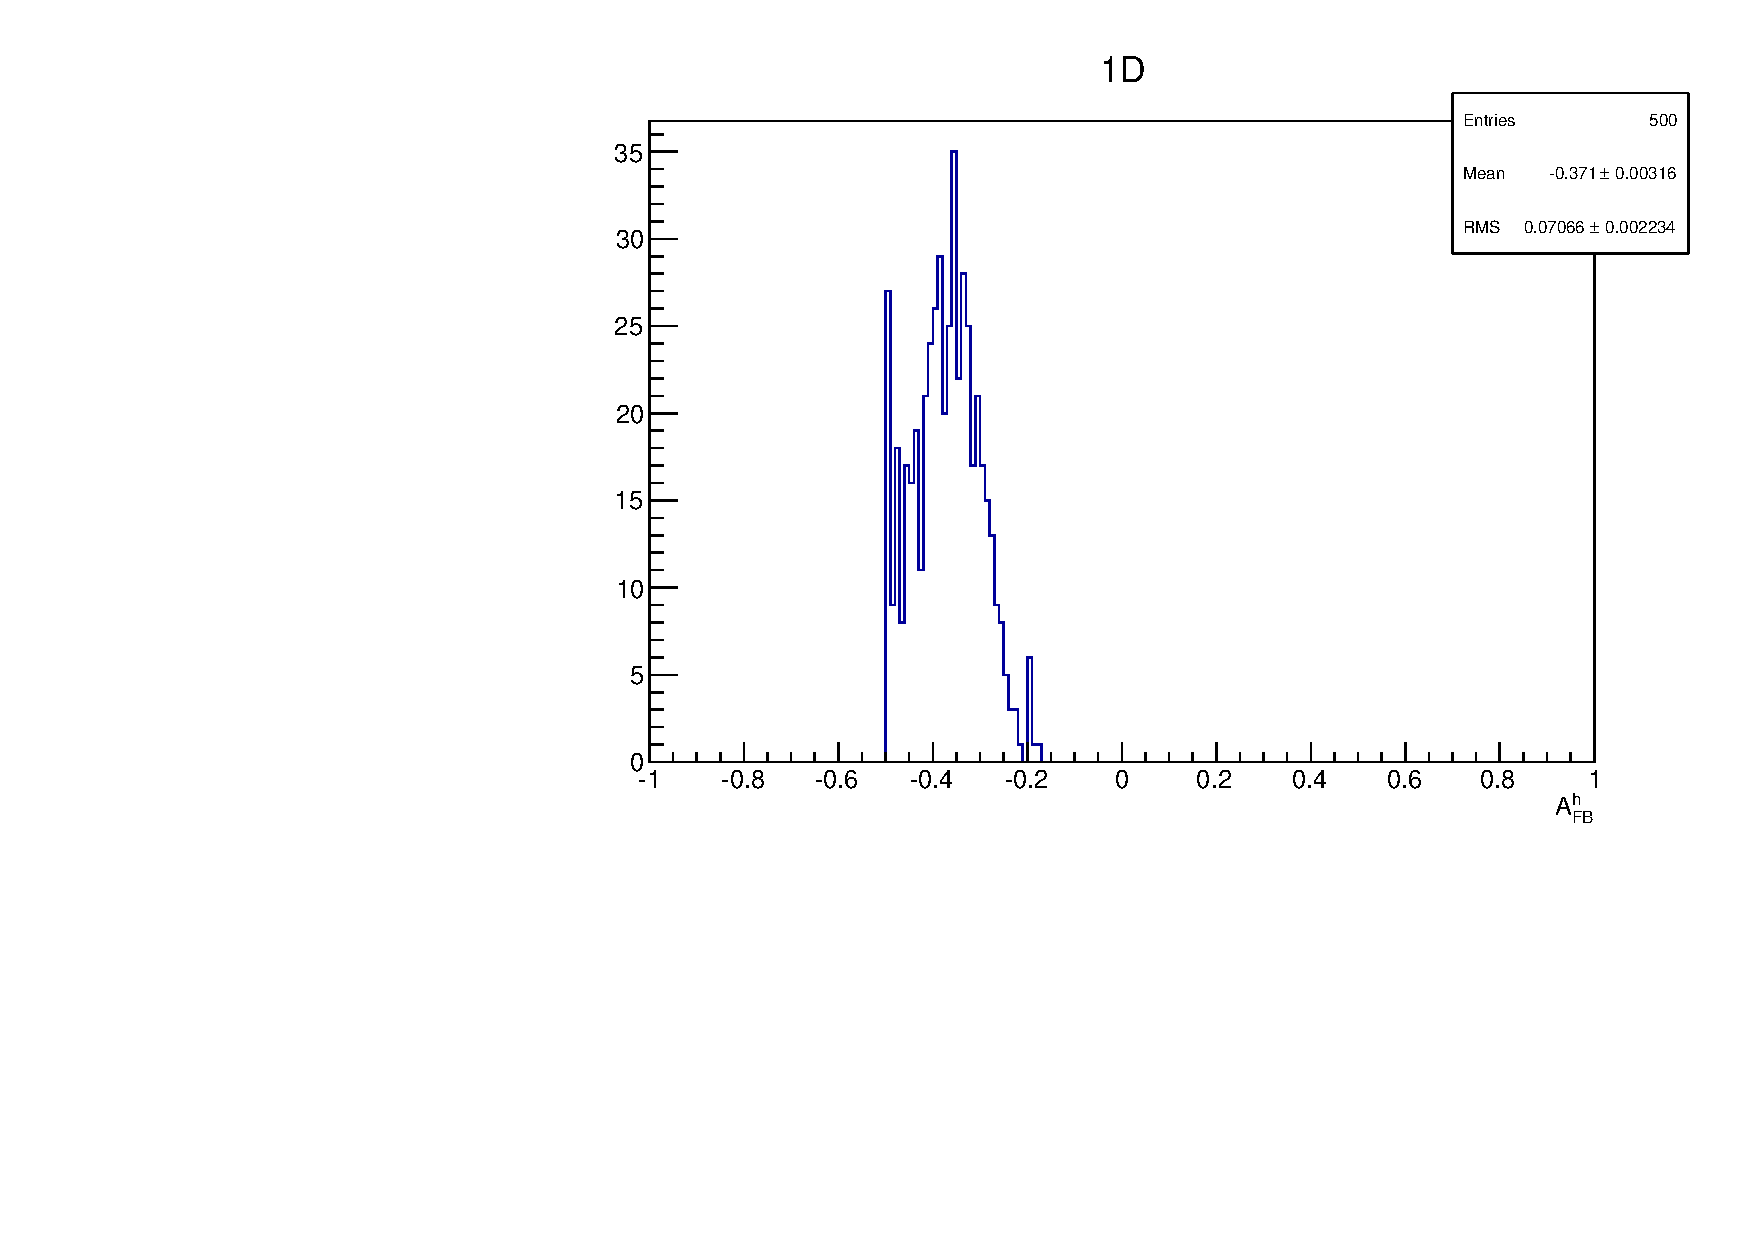
\includegraphics[width=0.32\textwidth]{Lmumu/figs/toys3D/B1/1D/toys3D_afbB.pdf}
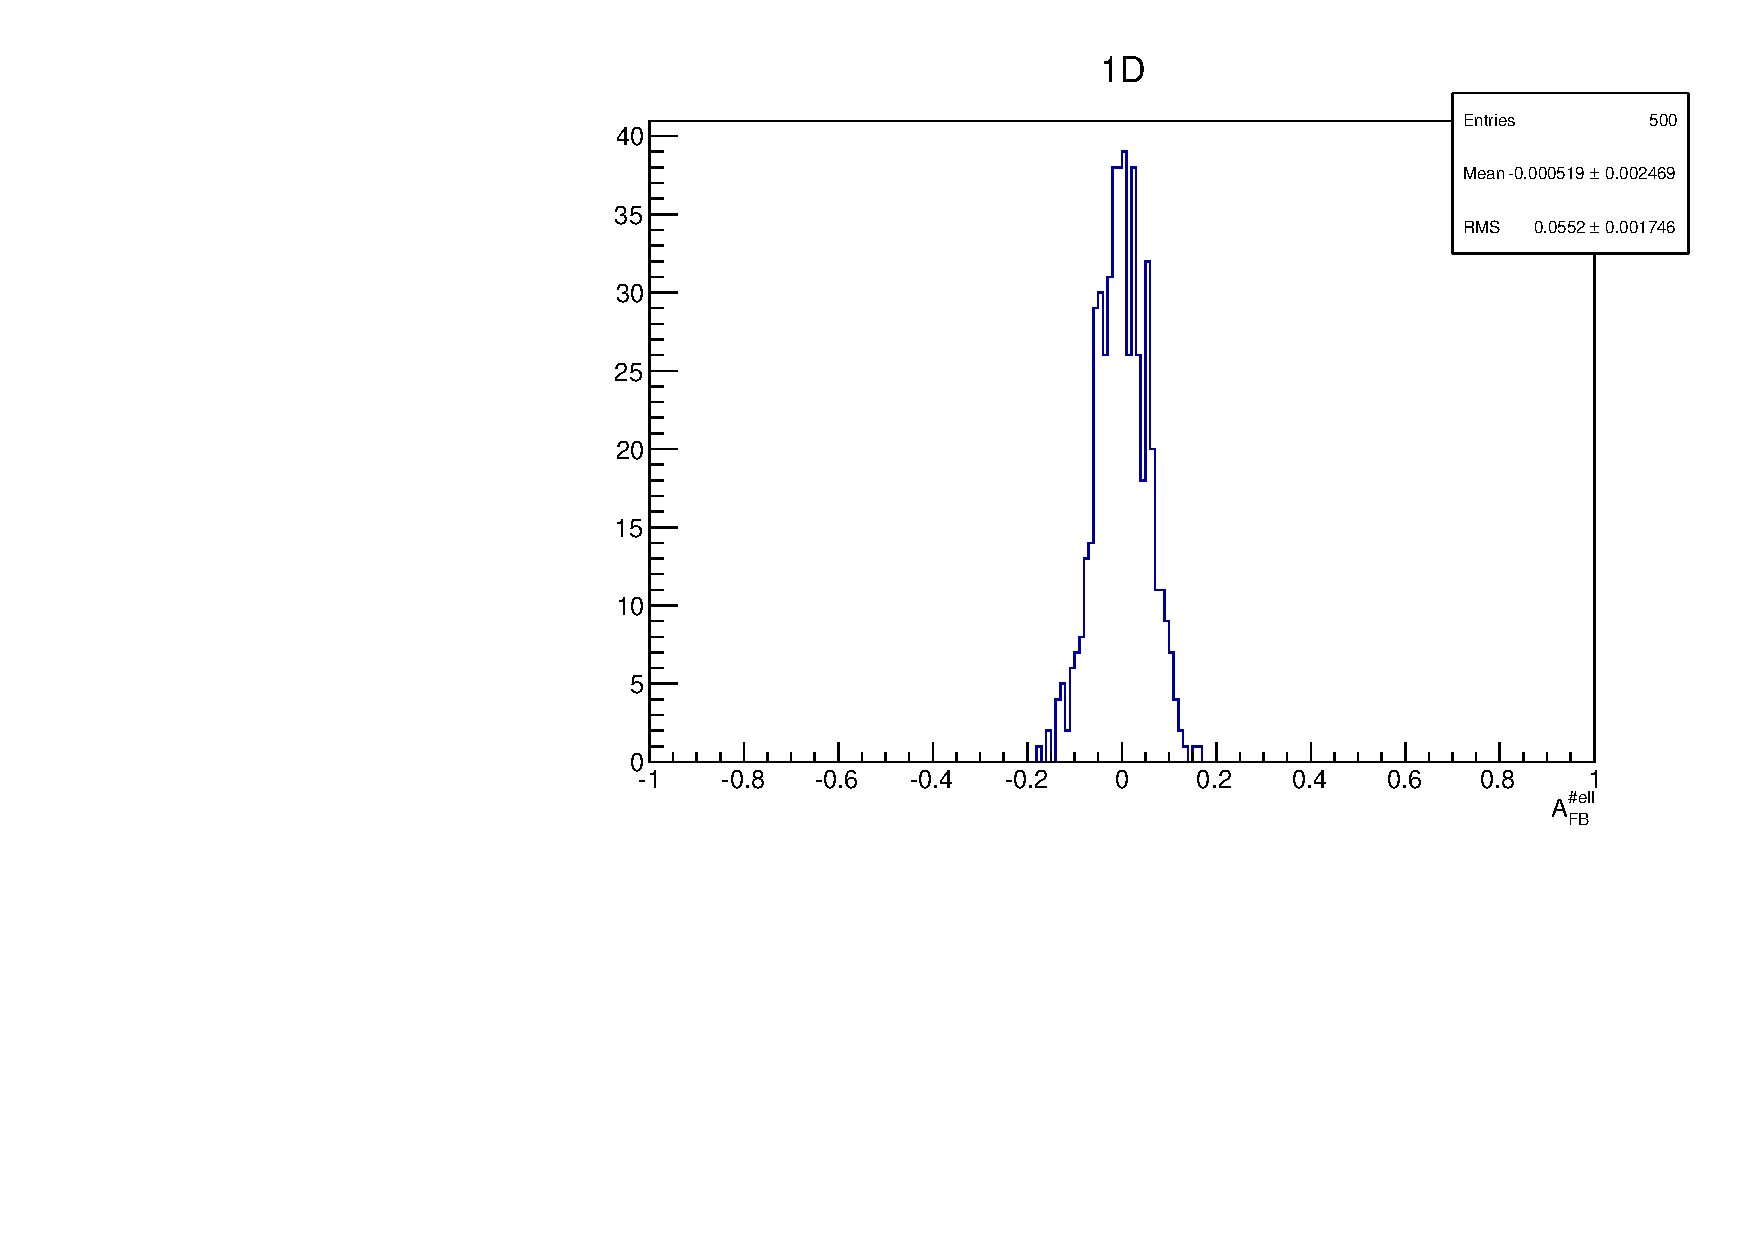
\includegraphics[width=0.32\textwidth]{Lmumu/figs/toys3D/B1/1D/toys3D_afb.pdf}
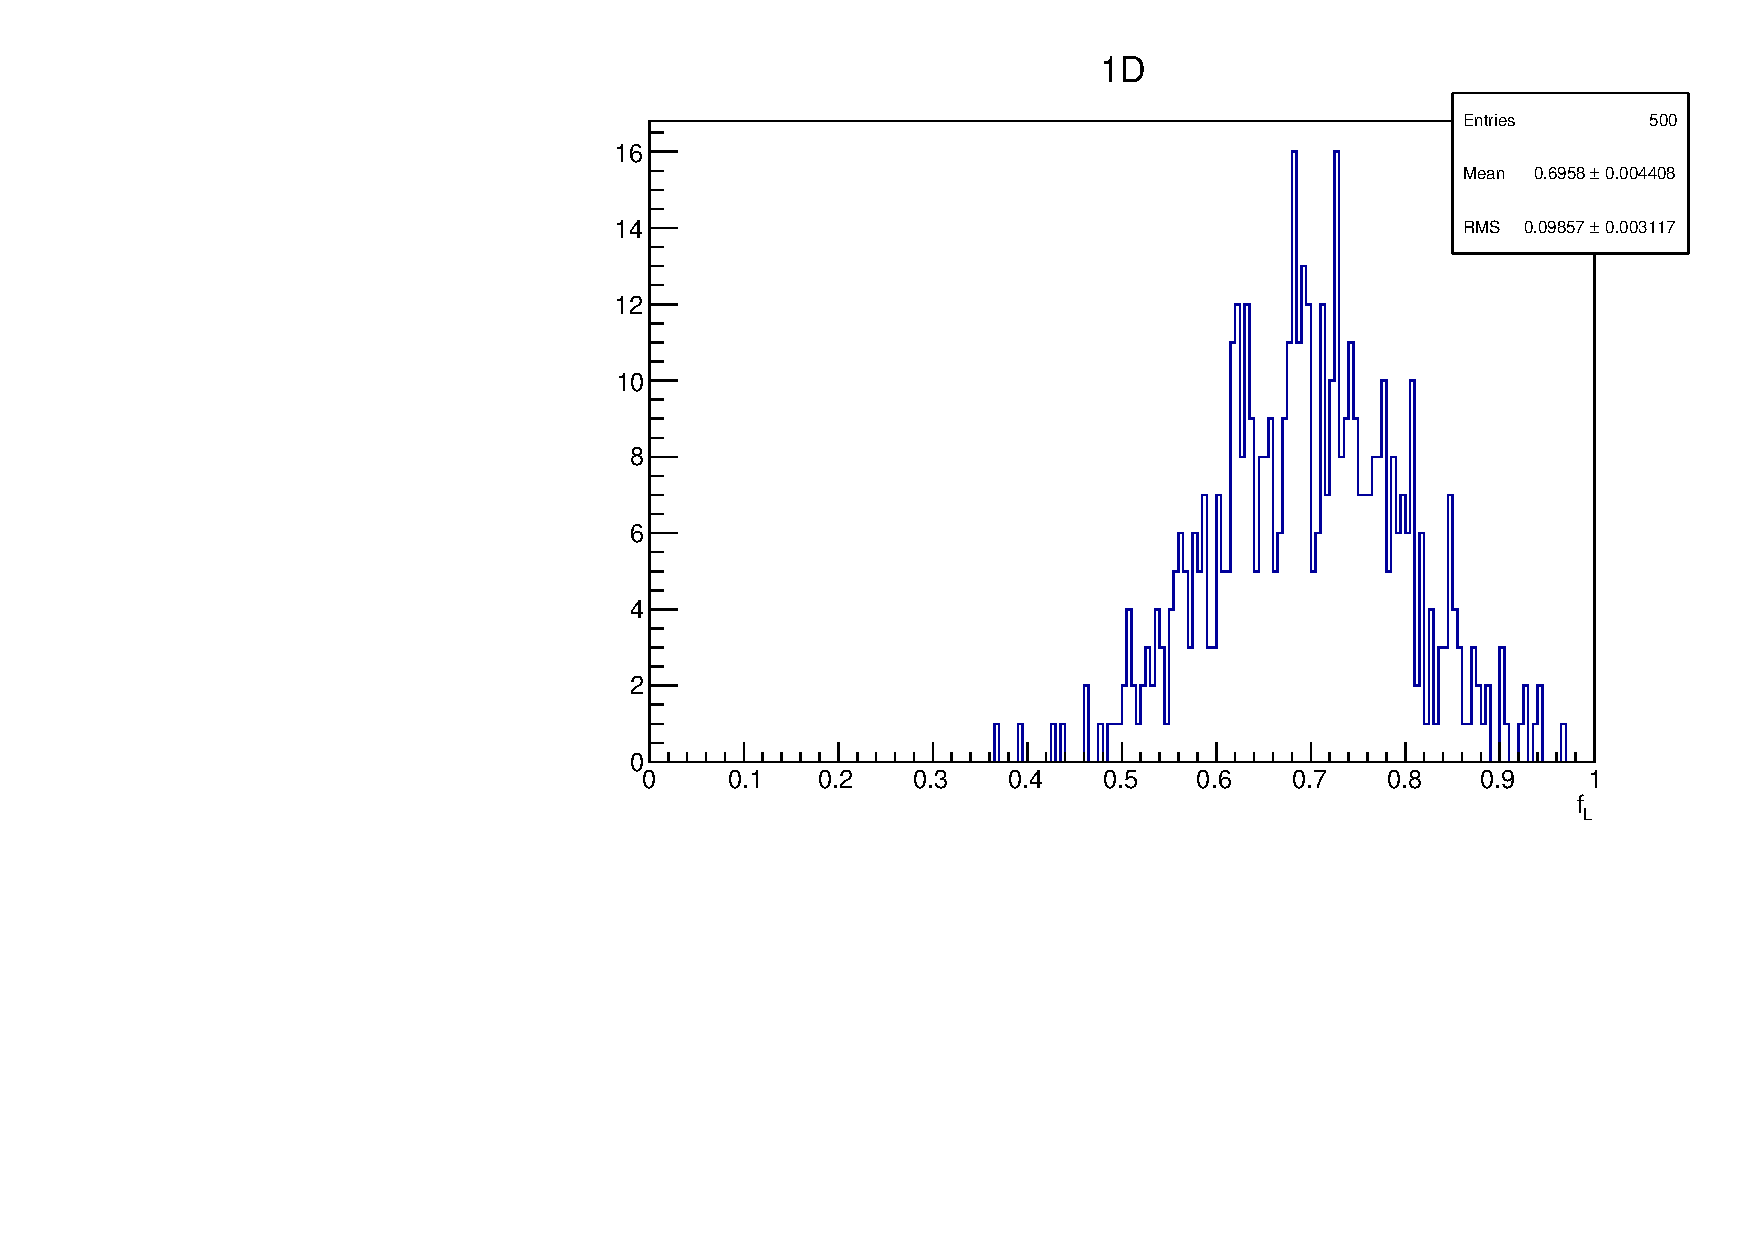
\includegraphics[width=0.32\textwidth]{Lmumu/figs/toys3D/B1/1D/toys3D_fL.pdf} \\
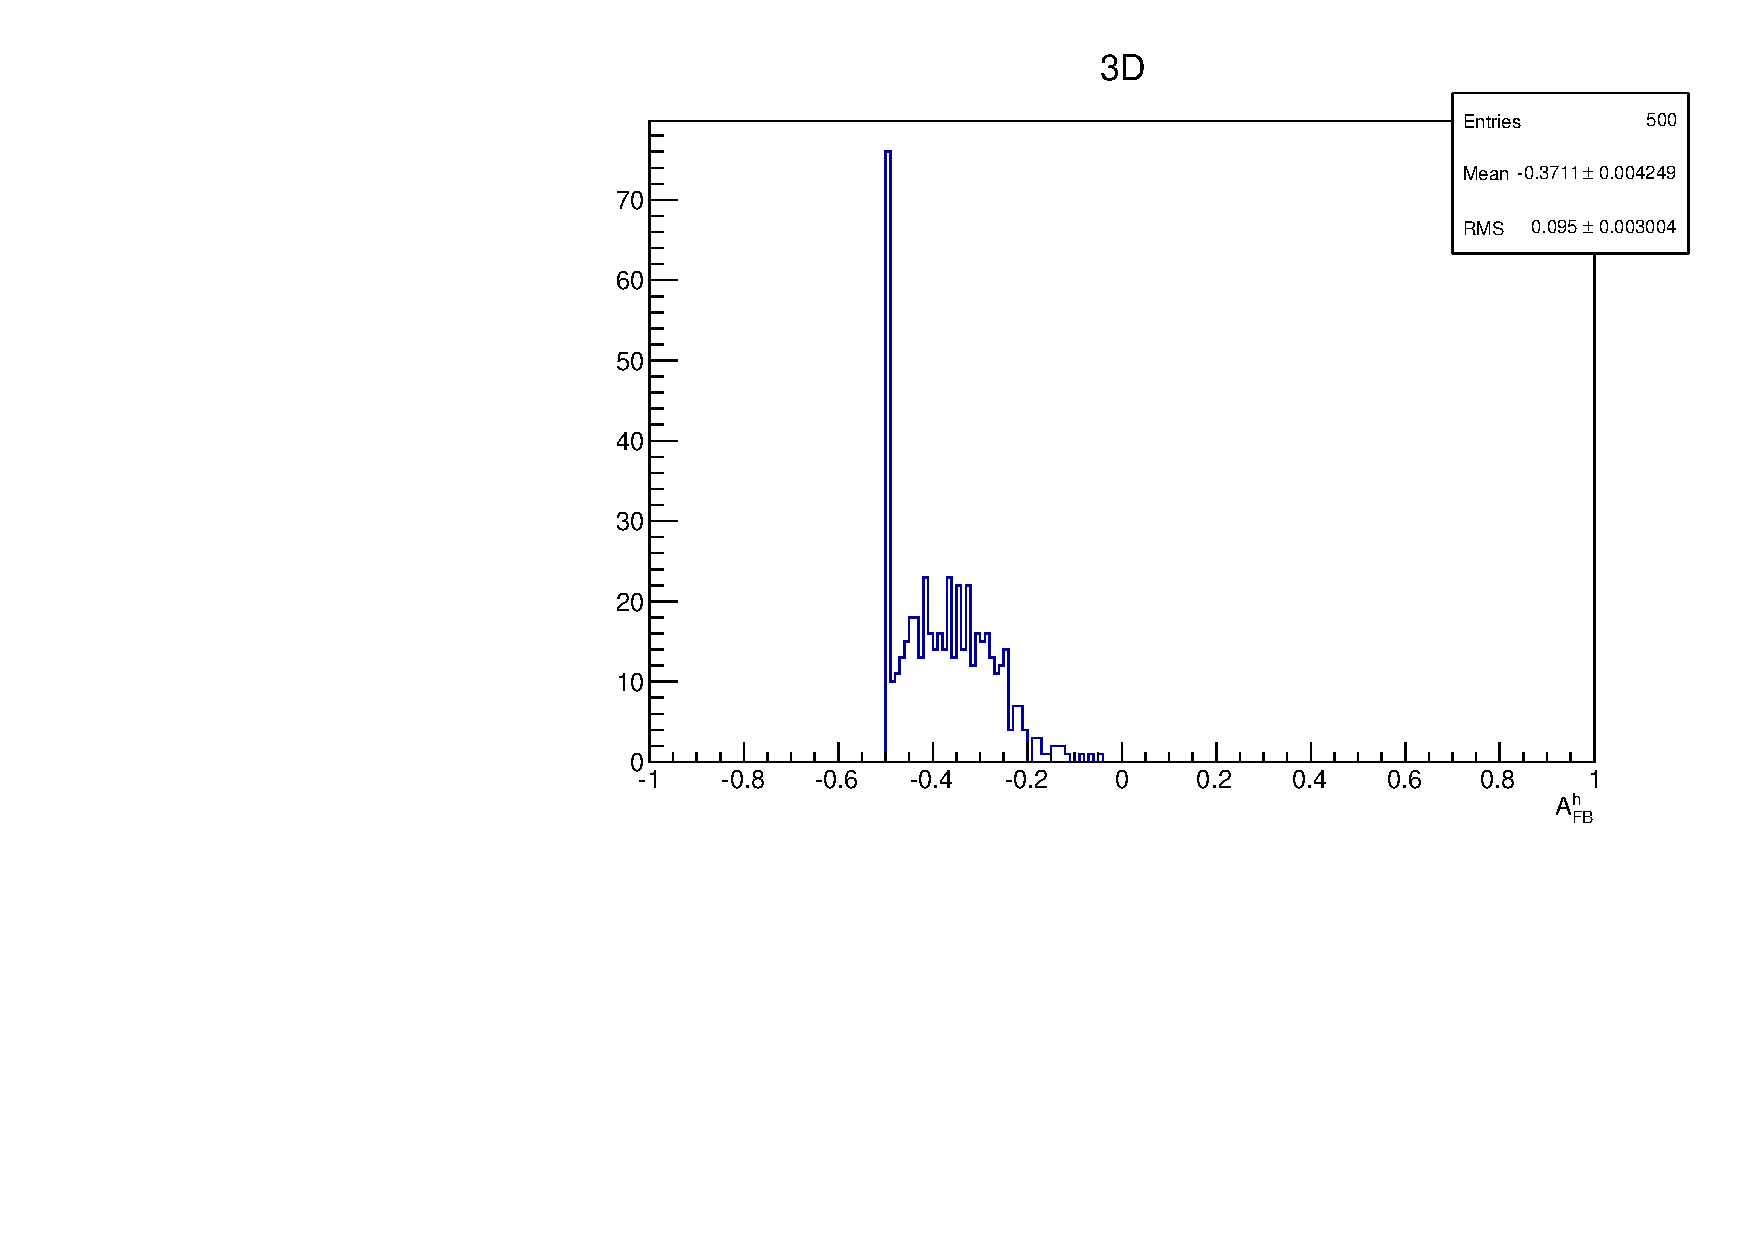
\includegraphics[width=0.32\textwidth]{Lmumu/figs/toys3D/B1/3D/toys3D_afbB.pdf}
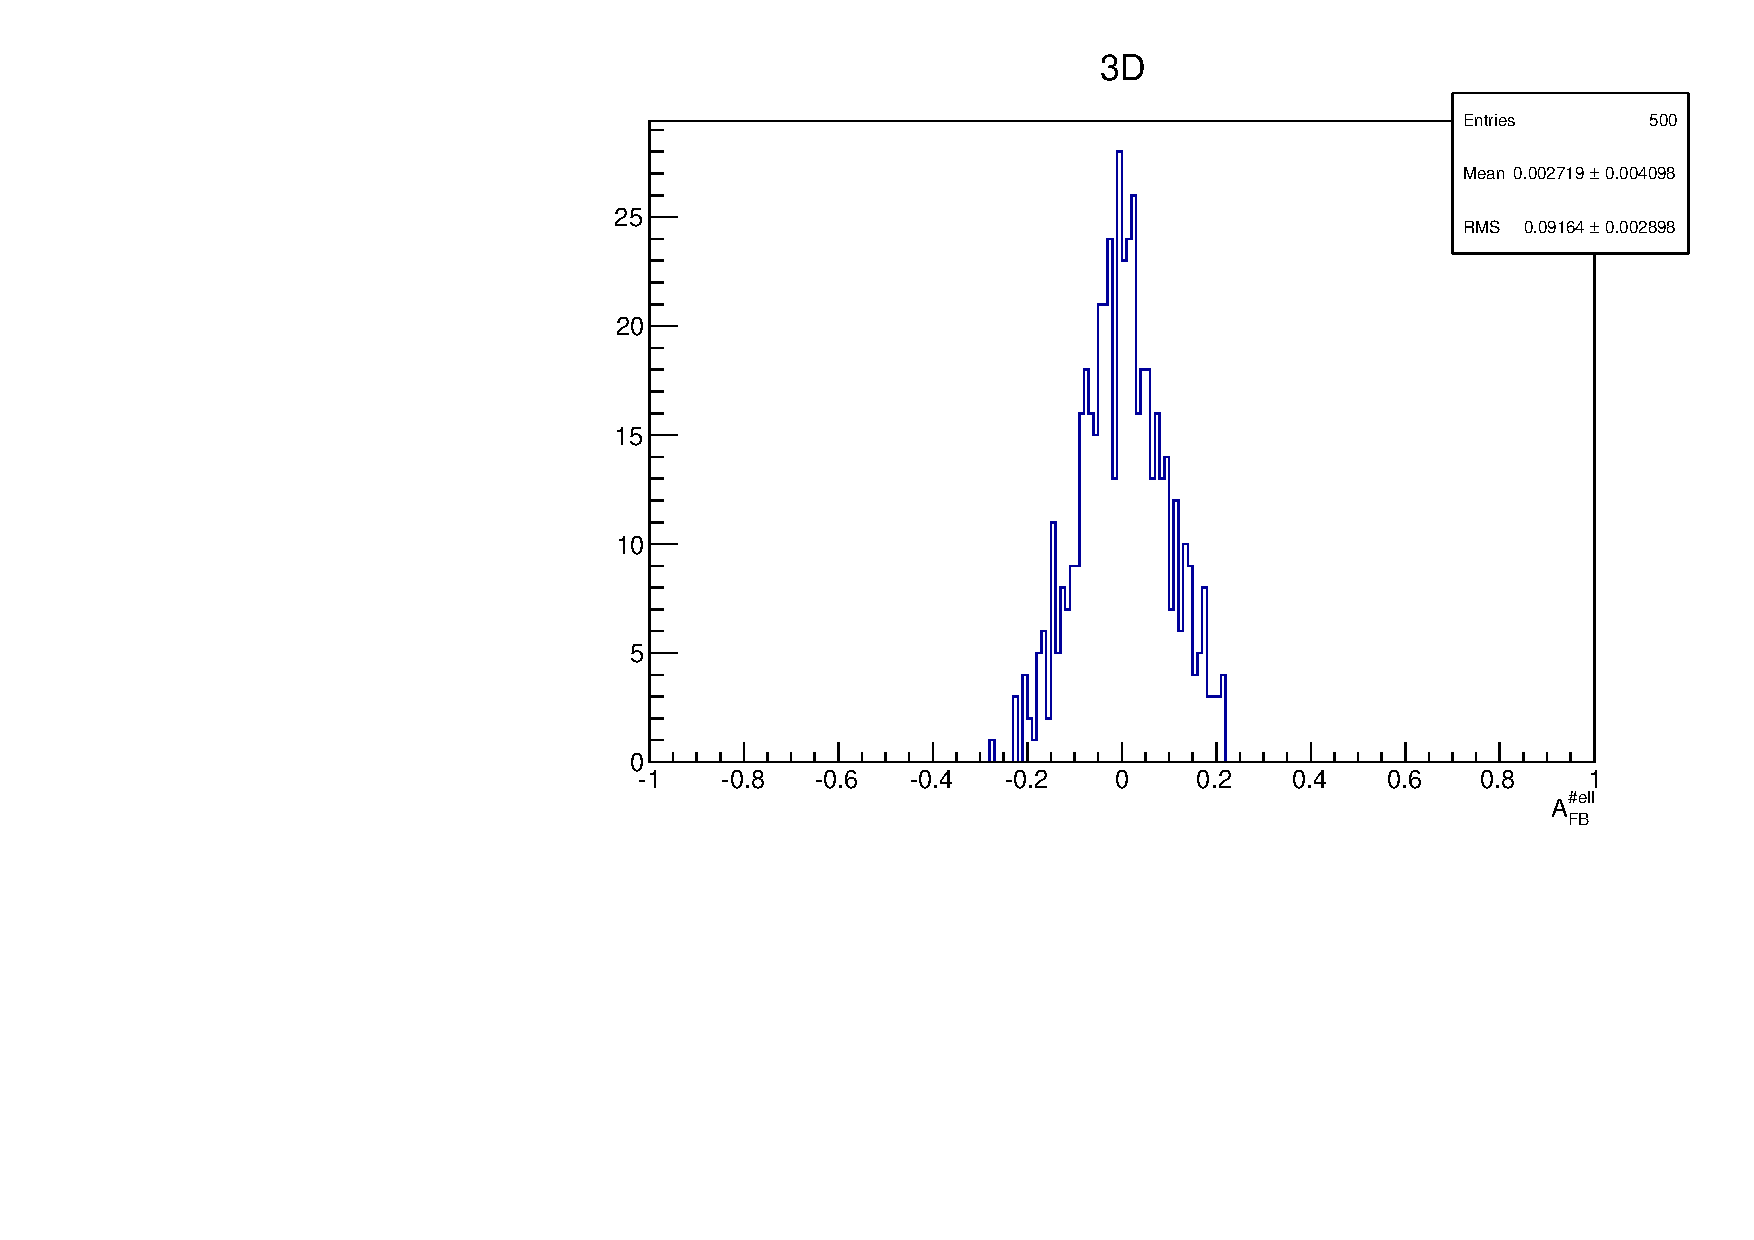
\includegraphics[width=0.32\textwidth]{Lmumu/figs/toys3D/B1/3D/toys3D_afb.pdf}
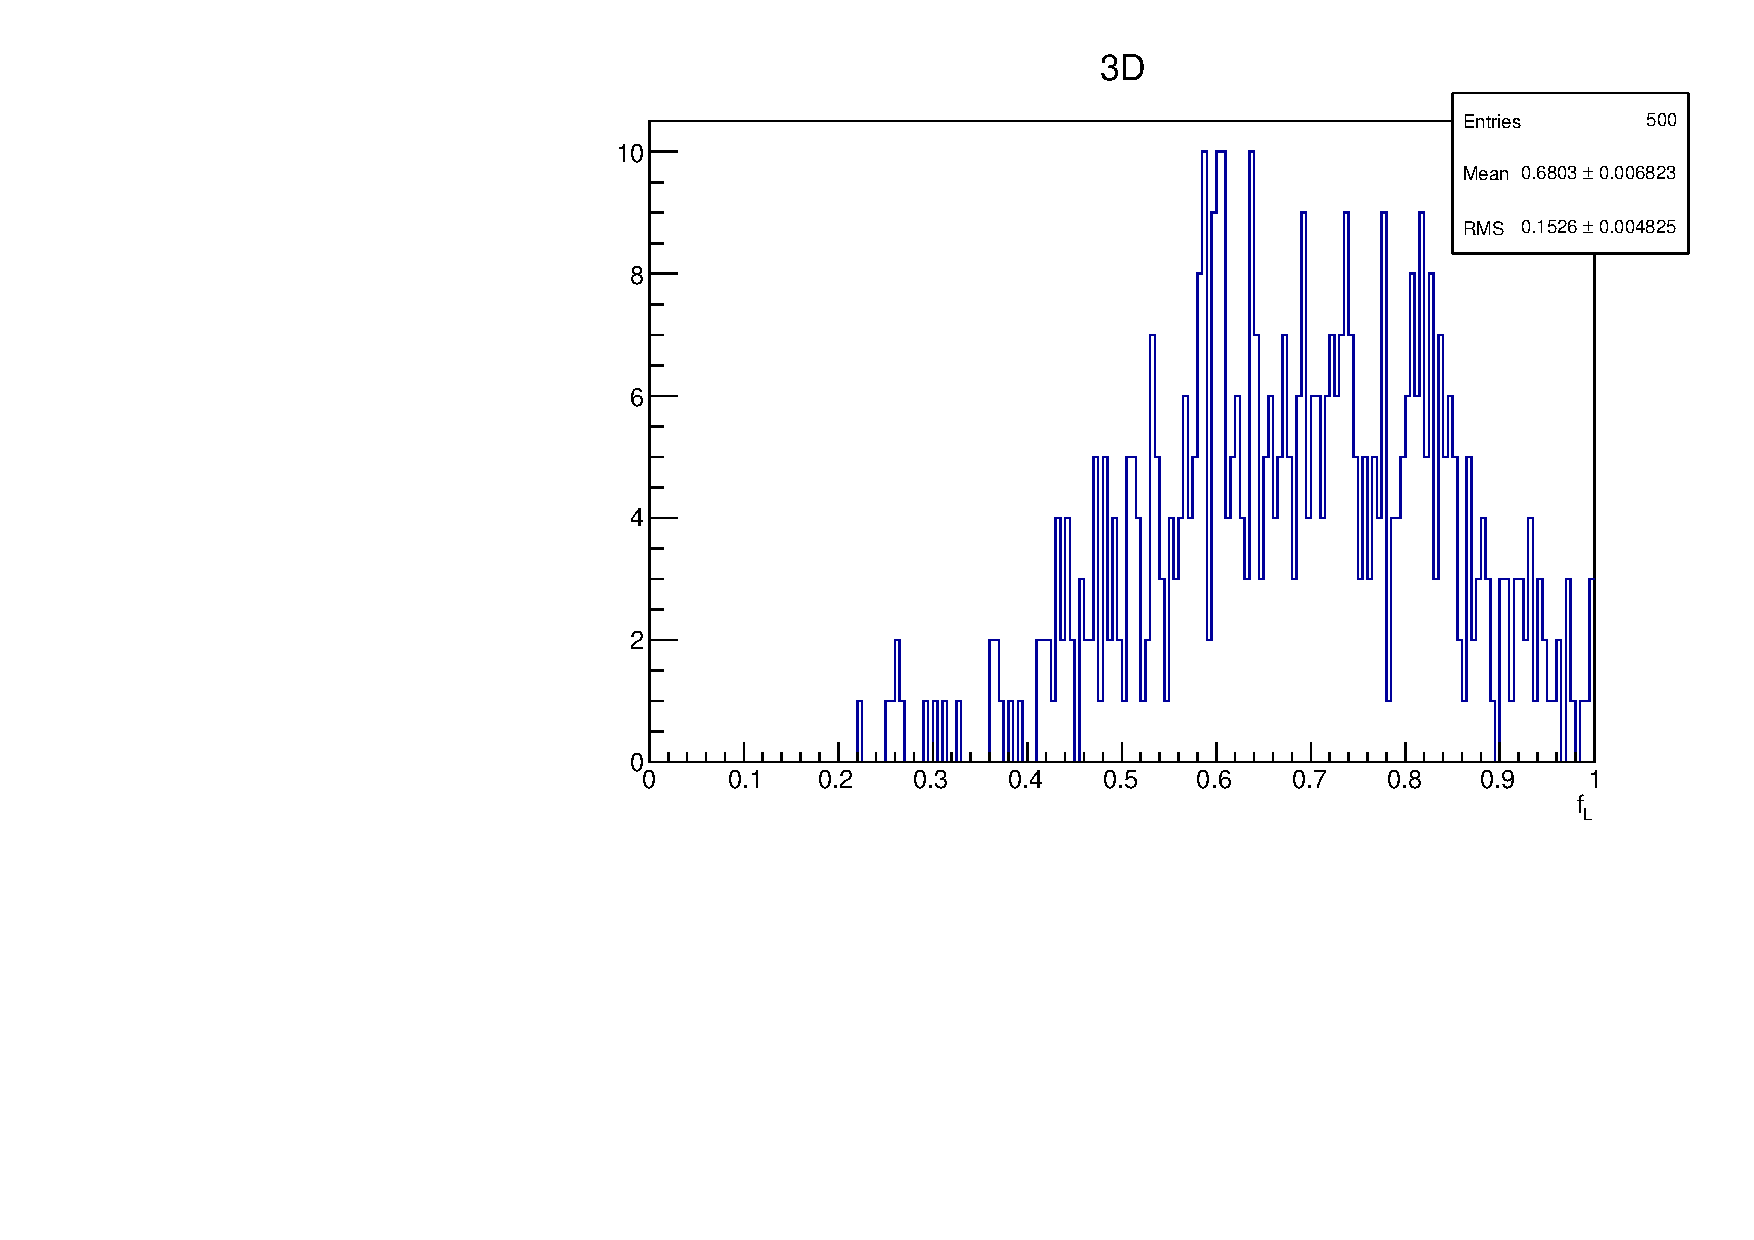
\includegraphics[width=0.32\textwidth]{Lmumu/figs/toys3D/B1/3D/toys3D_fL.pdf} \\
\caption{Distribution of oberved parameters of interest over 500 pseudo-experiments obtained
using the 1D fit method (top) and the 3D one (bottom). These toys correspond to events
generated with parameters and statistics corresponding to what is observed in the 15--20 \qsq nterval. }
\label{fig:3DtoyResults}
\end{figure}
%
\begin{figure}[h]
\centering
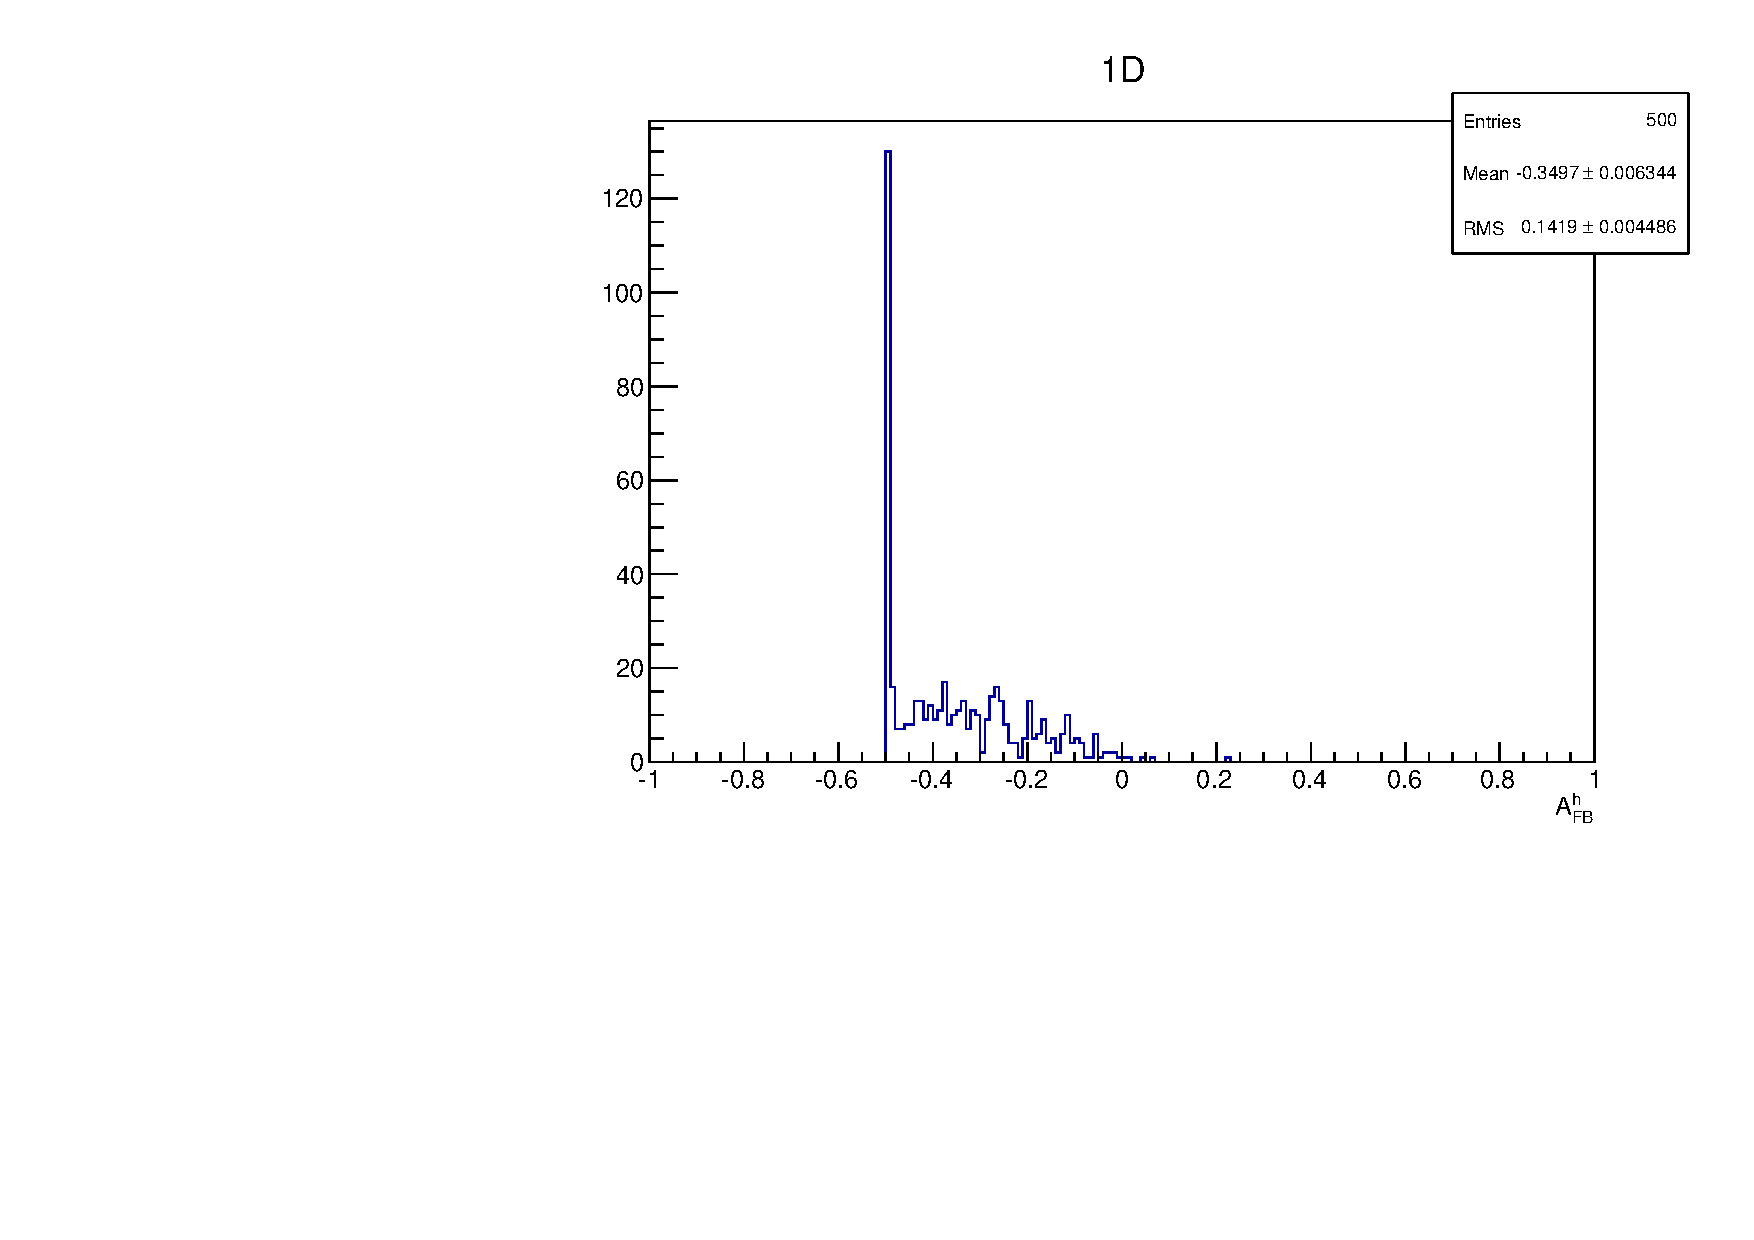
\includegraphics[width=0.32\textwidth]{Lmumu/figs/toys3D/B2/1D/toys3D_afbB.pdf}
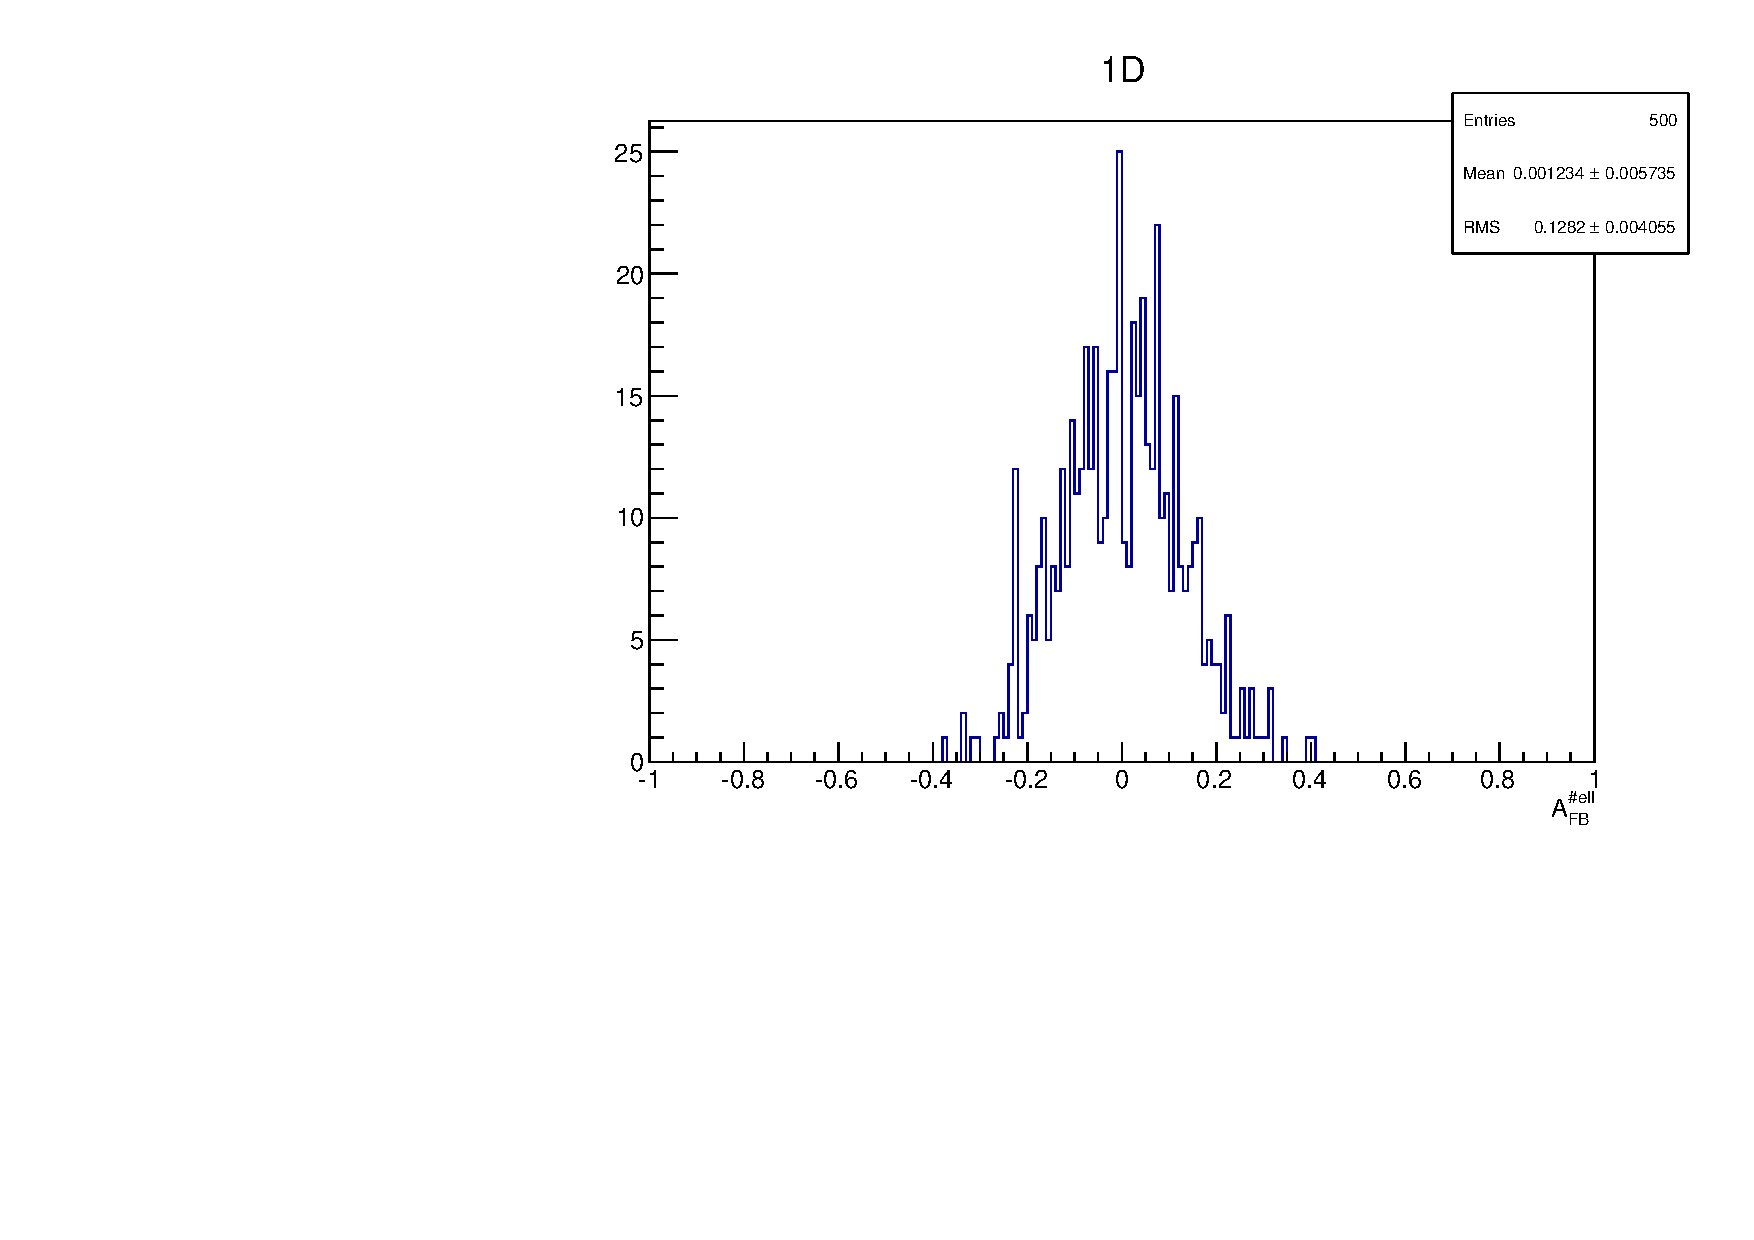
\includegraphics[width=0.32\textwidth]{Lmumu/figs/toys3D/B2/1D/toys3D_afb.pdf}
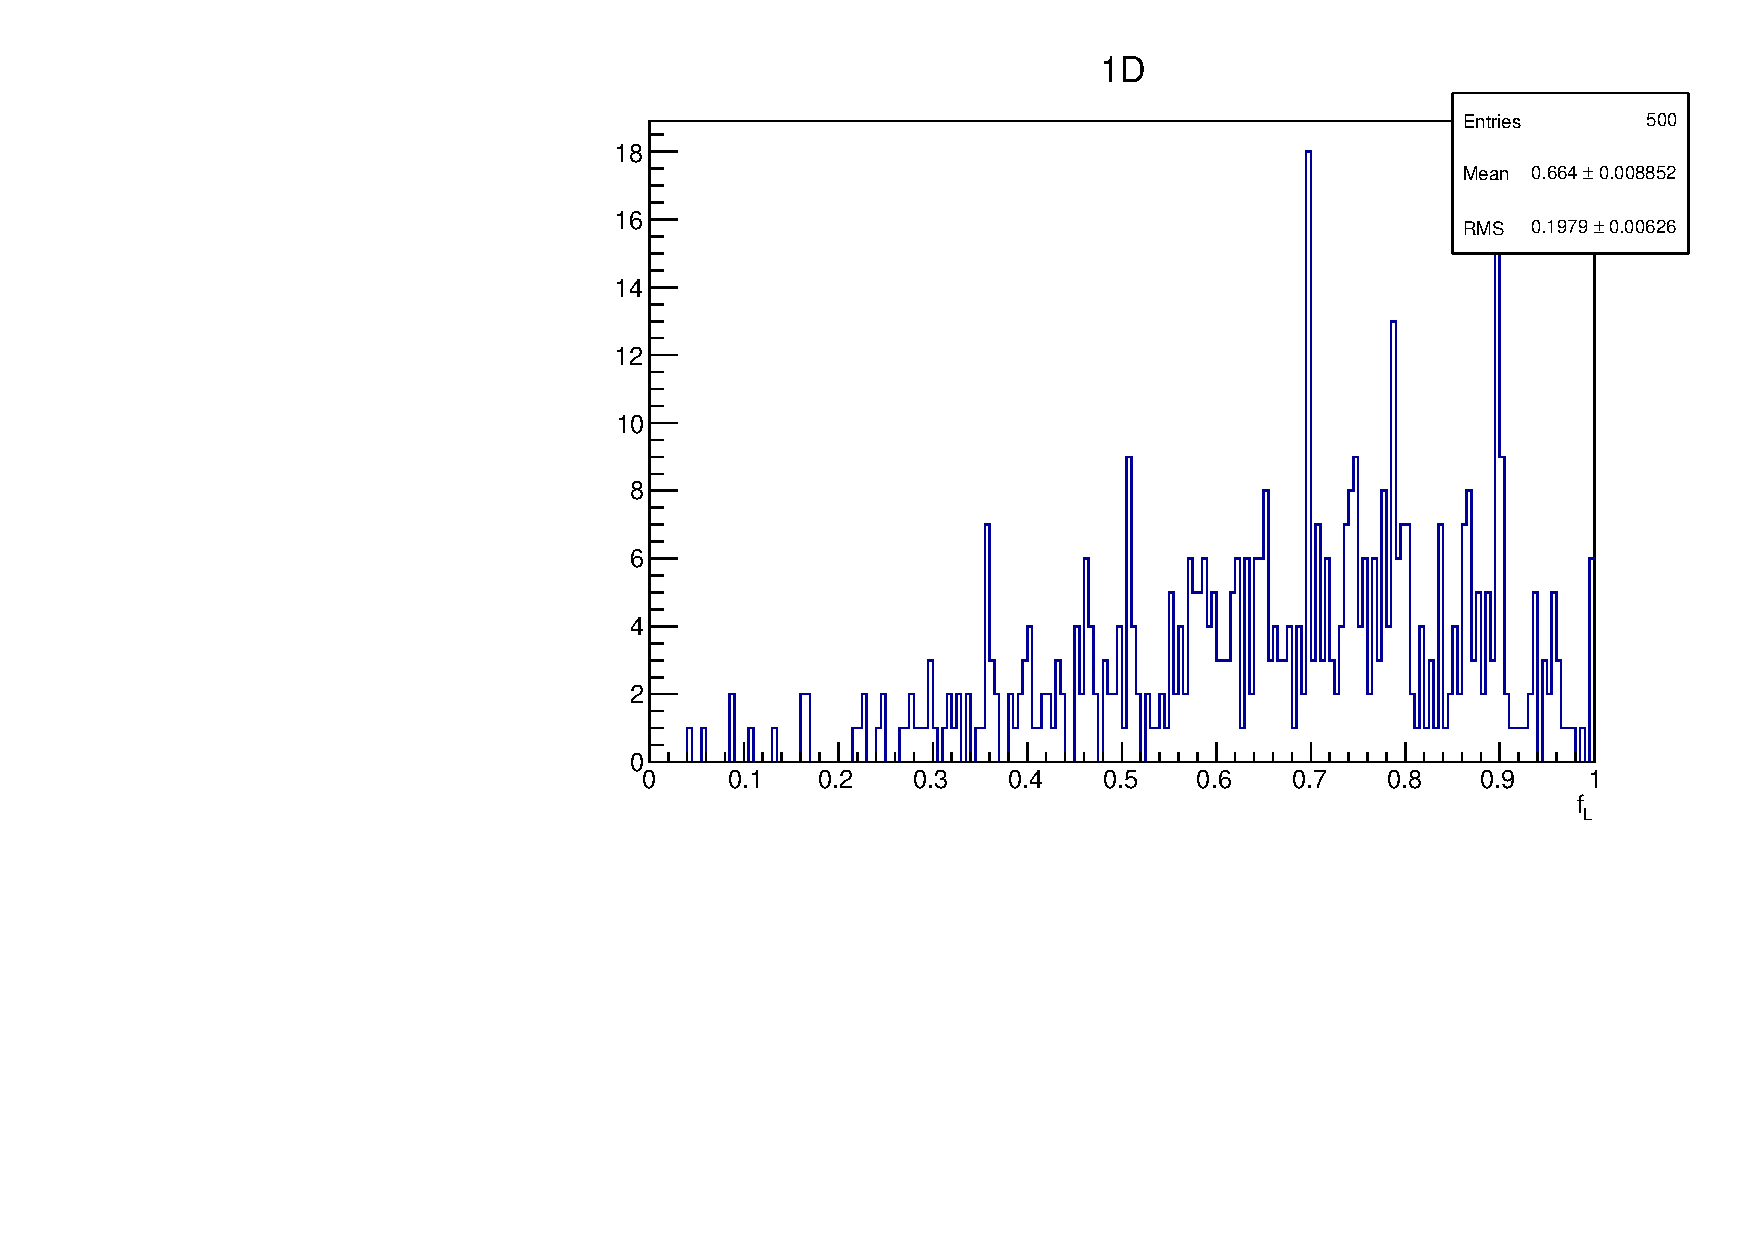
\includegraphics[width=0.32\textwidth]{Lmumu/figs/toys3D/B2/1D/toys3D_fL.pdf} \\
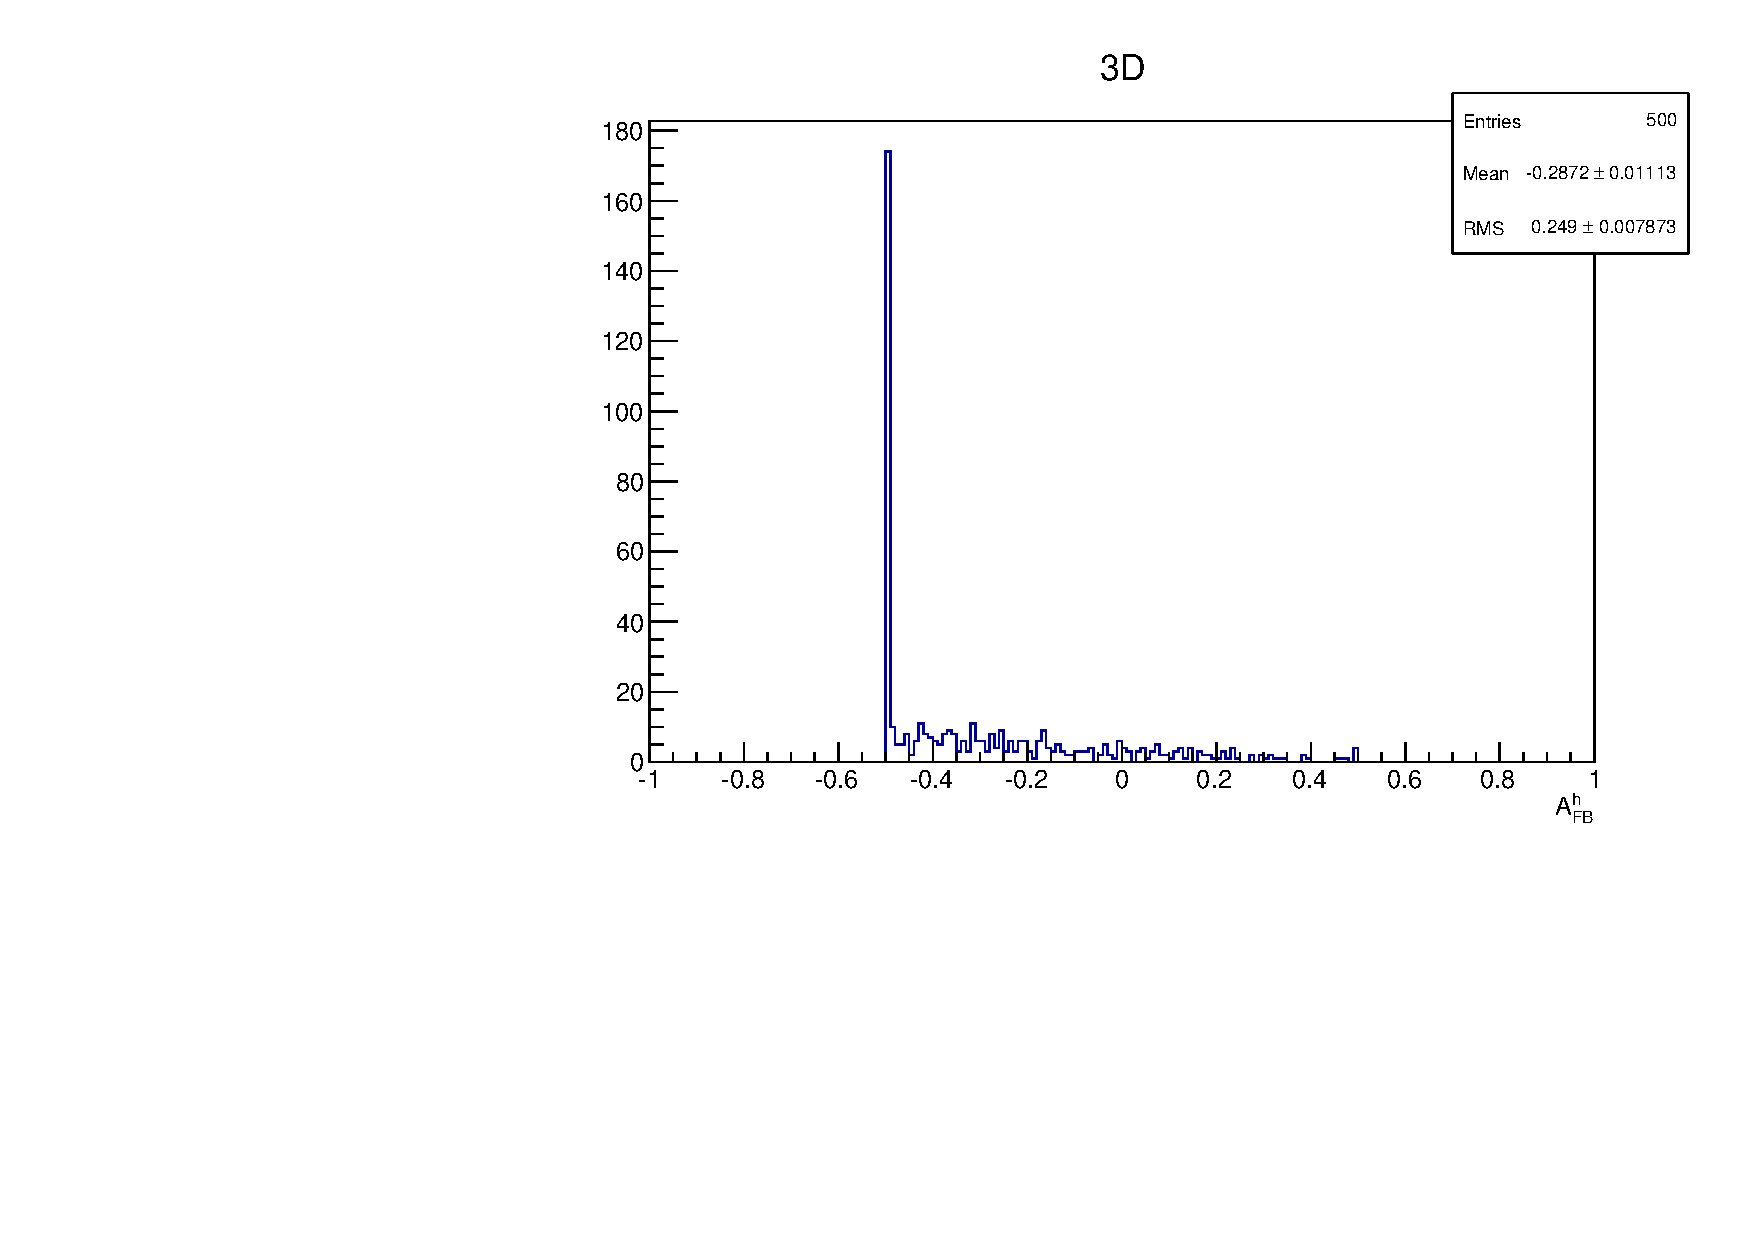
\includegraphics[width=0.32\textwidth]{Lmumu/figs/toys3D/B2/3D/toys3D_afbB.pdf}
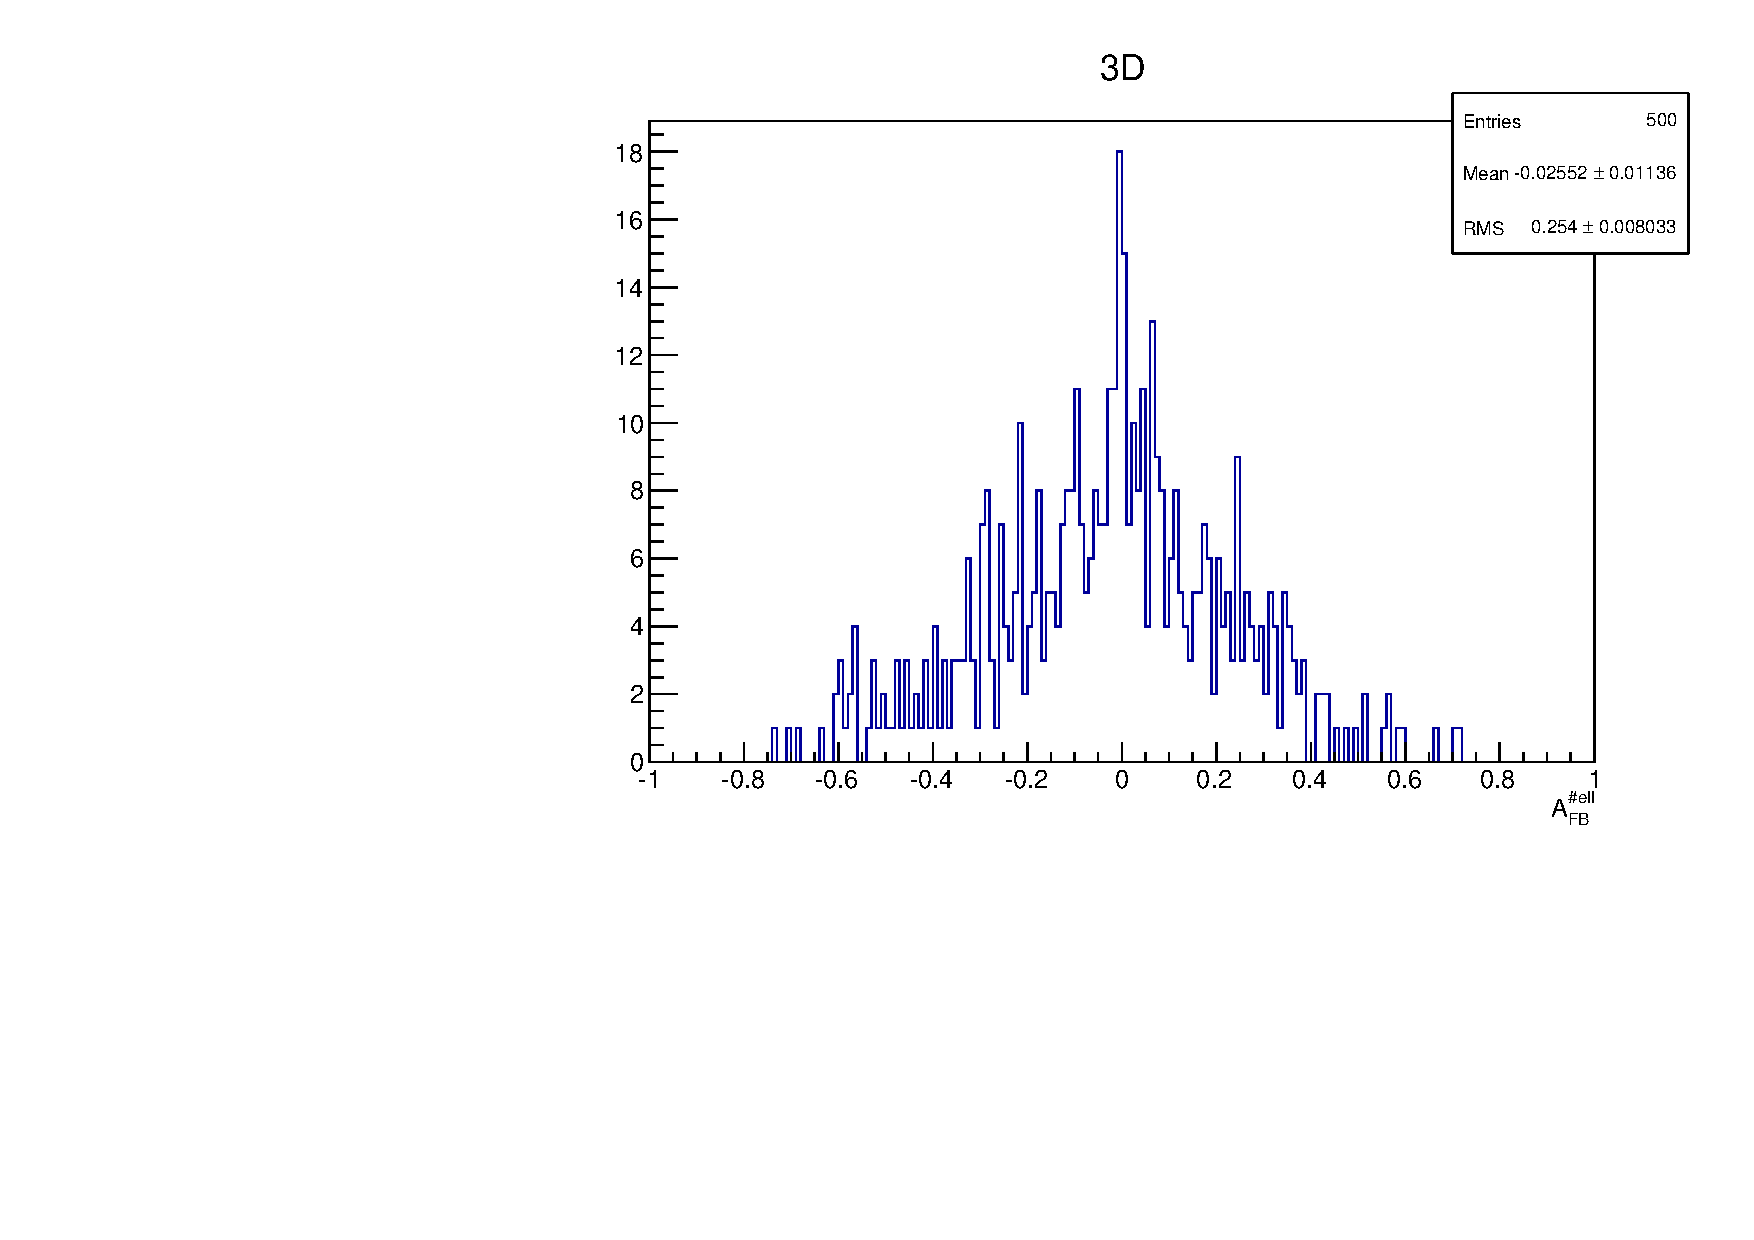
\includegraphics[width=0.32\textwidth]{Lmumu/figs/toys3D/B2/3D/toys3D_afb.pdf}
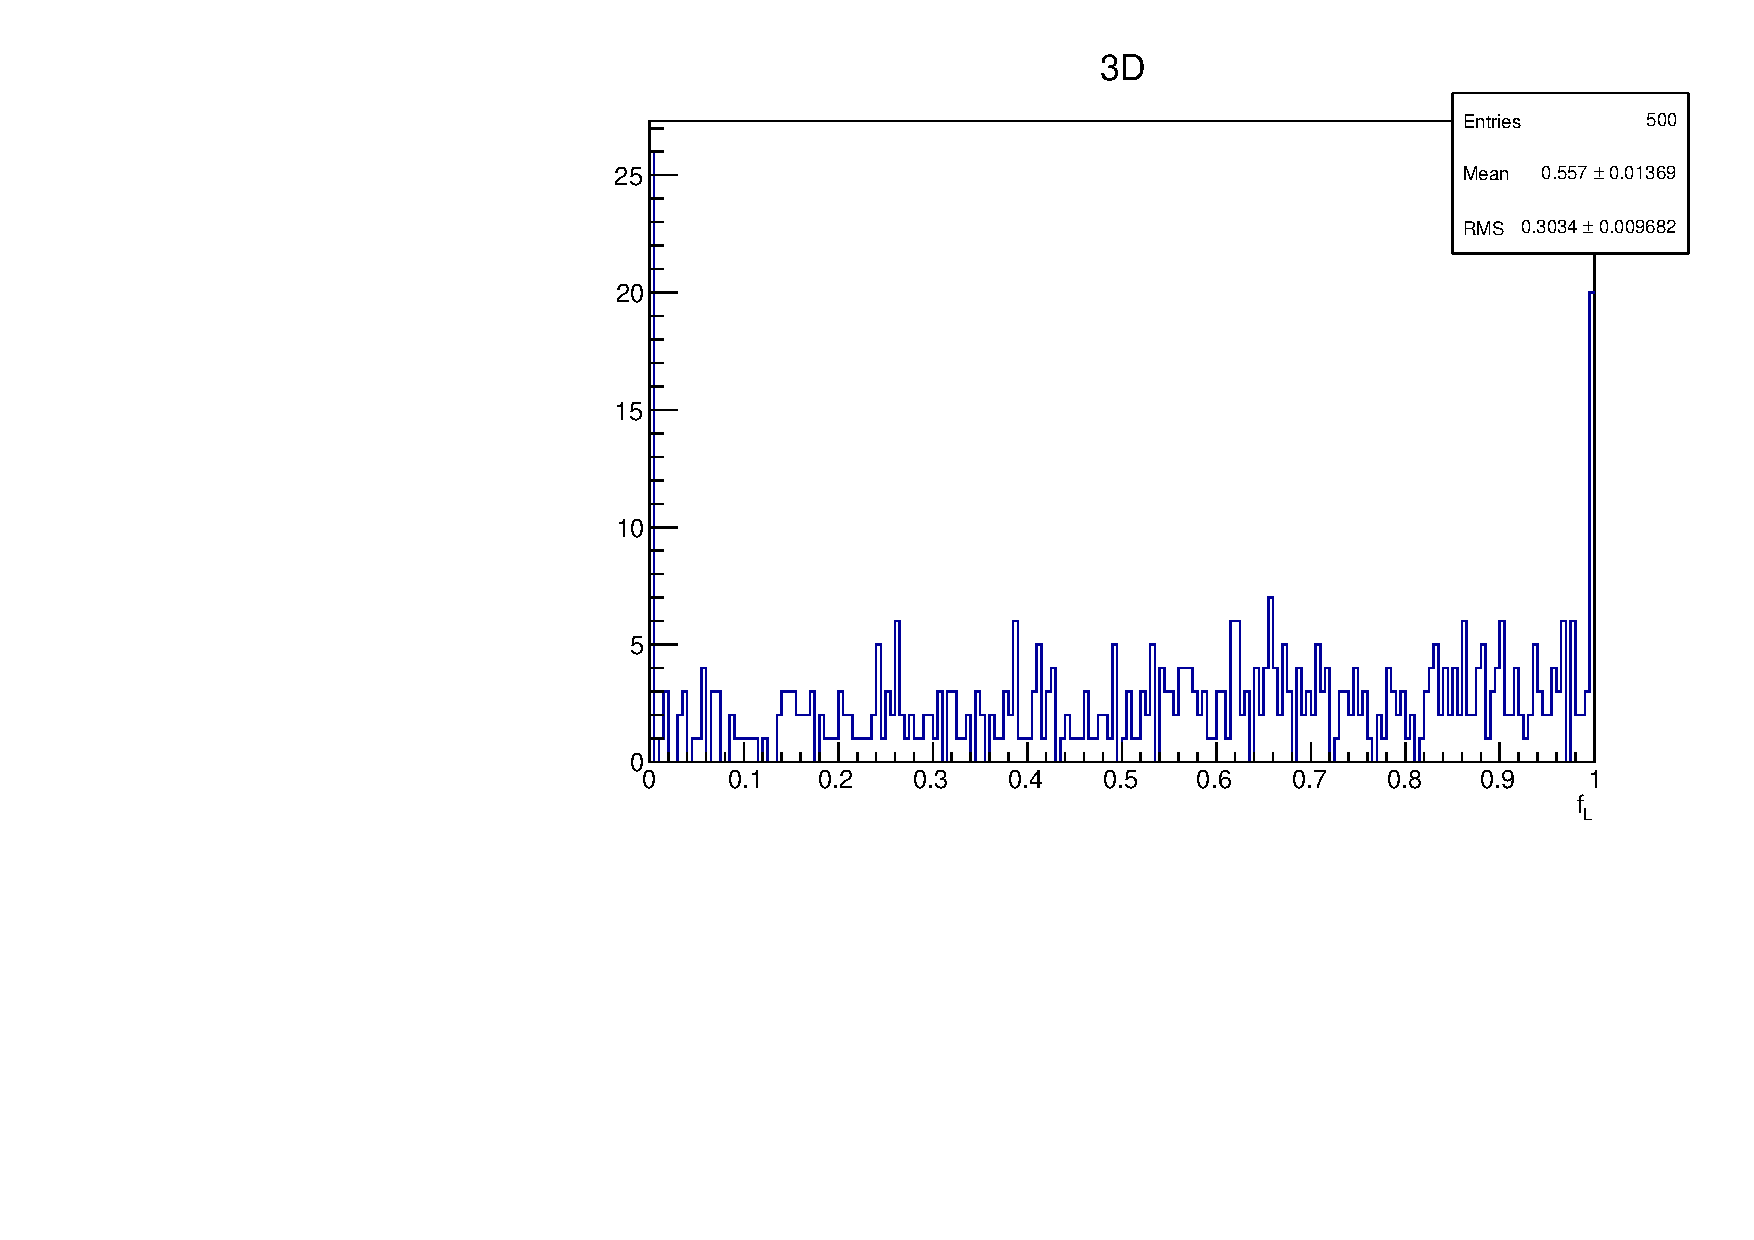
\includegraphics[width=0.32\textwidth]{Lmumu/figs/toys3D/B2/3D/toys3D_fL.pdf} \\
\caption{Distribution of oberved parameters of interest over 500 pseudo-experiments using the 1D fit
method (top) and the 3D one (bottom). These toys correspond to events generated with parameters
and statistics corresponding to what we observe in the 11--12.5 \qsq interval. }
\label{fig:3DtoyResults_lowest_stats}
\end{figure}


%In all cases we notice a slight bias in the fitting result. There fore we 
%assign as a systematic the full difference we observe on toys.
%Values of the systematic are reported in table \ref{tab:biassys} in bins of \qsq.

%\begin{table}
%\centering
%\begin{tabular}{lcccc} \hline\hline
%\qsq bin    &   $A_{\rm FB}^\ell$			&  		 $f_{\rm L}$ 	 			 &		 $A_{\rm FB}^h$  		 \\
%\hline
%0.1-2.0		&	$-0.01126 \pm 0.01272$  &  $-0.14299 \pm 0.01551$    &  $0.04002 \pm 0.00950$    \\
%11.0-12.5	&	$0.00123 \pm 0.00574$	&  $-0.03601 \pm 0.00885$	 &  $0.02030 \pm 0.00634$  	\\
%15.0-16.0	&	$0.00592 \pm 0.00555$	&  $-0.03112 \pm 0.00880$	 &  $0.00772 \pm 0.00577$  	\\
%16.0-18.0	&	$0.00973 \pm 0.00389$	&  $0.00115 \pm 0.00634$	 &  $-0.00161 \pm 0.00428$  	\\
%18.0-20.0	&	$-0.00400 \pm 0.00391$	&  $-0.00306 \pm 0.00728$	 &  $0.00258 \pm 0.00458$  	\\
%\hline
%15.0-20.0	&	$-0.00052 \pm 0.00247$  &  $-0.00424 \pm 0.00441$     &  $-0.00100 \pm 0.00316$   \\
%\hline
%\end{tabular}
%\caption{Absolute values of systematic undertainties due to fit bias in bins of \qsq.}
%\label{tab:biassys}
%\end{table}



